\documentclass[rgb,listoffigures,listoftables,final]{cam-thesis}

% Packages go here

% Document Details
\title{An Efficient Quantum Message Authentication Scheme}
\author{Nicolas Perez}
\date{August 2022}
\thesistype{thesis}
\submittedto{the Faculty of Graduate and Postdoctoral Affairs}
\degree{Master}
\program{Computer Science}
\college{Carleton University}
\location{Ottawa, Ontario}
\submissiondate{2022}

% PDF meta-info:
\subjectline{\@title}
\keywords{keyword 1, keyword 2, etc.}

\abstract{%
Quantum networking is the study of transmitting data that uses quantum mechanics principles (quantum messages). Quantum networking aims to connect two or more quantum computers over a network to cooperatively increase their capabilities, much like how the internet connects computers today. This thesis describes an algorithm that detects when an adversary maliciously modifies a quantum message (an integrity attack). The algorithm is analyzed in terms of its ability to detect an integrity attack and its efficiency in terms of classical computational complexity and the number of quantum gates used. It is rigorously compared to the Clifford code quantum message authentication (QMA) scheme. It offers a trade-off compared to the Clifford code QMA scheme in terms of integrity detection versus efficiency: reduced detection rates and improved efficiency. The new algorithm is not proven to be a QMA scheme, as the proof of its security is restricted to Pauli attacks (and is given as an approximation) and it has not been proven to encrypt data. Instead, it is conjectured to satisfy a more lax alternative definition of QMA. As a consequence of developing this new algorithm, a novel method for unranking permutations of multisets is also presented.
}

\acknowledgements{
 I am grateful for the support from my supervisors Evangelos Kranakis and Michel Barbeau, and the additional support from Joaquin Garcia-Alfaro. Their inquiry and feedback on my research throughout my degree have been very helpful. My supervisors were also eager to teach me quantum computing at the start of my degree, and ensured that I had a good foundation of knowledge for starting my research.

My girlfriend provided me with an immense amount of support in more ways than I can say. She, along with my cats Steve and Bucky, were an appreciated source of comfort and humour and kept me good company during the isolating times of the COVID pandemic.

I used to ask my dad repeatedly while I was a small child: "What doing dad, what doing?", whilst he was tinkering around. He would let me watch and explain to me what he was doing. I used to ask my mom repeatedly: "Why? Why? Why?", when asking her about how the world worked. She would try her best to answer my questions! Both of them helped me become curious and want to know more about the world.

I am thankful for the support of all my family and friends.
}

%\setcounter{tocdepth}{1}

%these two packages aren't loading properly
%\usepackage[table]{xcolor}
%\usepackage[hidelinks]{hyperref}
%\usepackage[
%backend=biber,
%style=alphabetic,
%]{biblatex}
\usepackage{chngpage}
\usepackage{epsfig}
\usepackage{graphics}
\usepackage{float}
\usepackage{graphicx}
\usepackage{alltt}
\usepackage{amssymb}
\usepackage{latexsym}
\usepackage{comment}
\usepackage{amsmath}
\usepackage{geometry}
\usepackage{url}
\DeclareMathOperator{\Tr}{Tr}
\usepackage{braket}
\usepackage{boldline}
\usepackage{apxproof}
\usepackage{setspace}
\newtheoremrep{myLemma}{Lemma}[section]

%call \ceil*{x} as per https://tex.stackexchange.com/questions/42271/floor-and-ceiling-functions
\usepackage{mathtools}
\DeclarePairedDelimiter{\ceil}{\lceil}{\rceil}
\DeclarePairedDelimiter{\floor}{\lfloor}{\rfloor}

%for algorithms
\usepackage{algorithm}
\usepackage{algpseudocode}
\algnewcommand\algorithmicforeach{\textbf{for each}}
\algdef{S}[FOR]{ForEach}[1]{\algorithmicforeach\ #1\ \algorithmicdo}

\usepackage{mathpazo} % math & rm
\usepackage{xltabular}

\def\changemargin#1#2{\list{}{\rightmargin#2\leftmargin#1}\item[]}
\let\endchangemargin=\endlist 

\newtheorem{theorem}{Theorem}[section]
\newtheorem{lemma}{Lemma}[section]
\newtheorem{corollary}{Corollary}[section]
\newtheorem{definition}{Definition}[section]
\newtheorem{example}{Example}[section]

\begin{document}

% Set up front matter (title page, toc, figures, etc.)
\frontmatter

% Input Chapters:
\chapter{Overview}
The new quantum message authentication scheme presented in this thesis will be referred to herein as the 'block Clifford code'. This chapter will outline what is presented in all the other chapters of this thesis.

Chapter~\ref{sec:Motivation} explains the motivation behind, and practical relevance of, the contents of this thesis. Chapter~\ref{sec:symbols} provides a table listing relevant symbols and their corresponding definitions. Chapter~\ref{sec:SummaryOfResults} summarizes the results of this thesis, by comparing the Clifford code and block Clifford code as well as briefly describing the efficiency of the novel multiset permutation unranking method. Chapter~\ref{sec:RequiredBackgroundKnowledge} goes over the necessary prerequisite knowledge for understanding the contents of this thesis. Chapter~\ref{sec:relatedWork} reviews related work, with a focus on the Clifford code. Chapter~\ref{sec:PerezCode} describes the block Clifford code. The novel multiset permutation unranking method is described in Subsection~\ref{subsubsection:keyMappings}, and is used in the key mapping process of the block Clifford code. The last chapter, Chapter~\ref{sec:Conclusion}, discusses the results of this thesis and potential future work.
% E.g. \input{ch-1-introduction}


\chapter{Motivation}
\label{sec:Motivation}
Quantum networking is like quantum computing's 'little brother', still very much new to the world and in its 'infancy'. The article, \emph{The Internet Goes Quantum}~\cite{popkin2021internet}, explains the motivations behind the emerging study of quantum networking and gives an interesting overview of current progress and main topics. In short, quantum computers have certain advantages over classical computers and enabling an internet for communicating quantum data will yield even more advantages. When mentioning the word 'classical' in this thesis, I am either using it to describe computation, a computer, or data concerning bits (what your typical modern computer uses). Authentication methods used on classical data must be fundamentally different than the ones applied to quantum data, due to the unique properties of quantum data~\cite{barnum2002authentication}. The emerging quantum internet thus puts pressure on the further development of QMA schemes.

Quantum data inherently has security properties, due to the 'no-cloning theorem' stating that quantum data can not be copied. Additionally, quantum data can only be read once by a computer, before its state is disturbed and irreversibly lost, and typically the information gained from reading the quantum data is only a small portion of its entirety (\cite{nielsen2002quantum}, see Box 12.1 for the no-cloning theorem and Subsection 2.2.3 for more info on quantum measurement). As a consequence, stolen quantum data has no perceivable use for the one who stole it, unless the characteristics of the data are known ahead of time. One could then assume that the most significant security threat to quantum data is modifying its contents. The method developed in this thesis is designed to detect an adversary modifying the contents of a quantum message.

The main goal of this thesis is to further advance the security capabilities of the quantum networks of the future. Some of the ideas on detecting integrity attacks may also one day apply to securing information in quantum computers, not just in quantum communications. This thesis describes a new solution for securing quantum data that shows improved efficiency, in terms of gates used and time complexity, compared to a similar QMA method. Efficiency may be paramount in applications with constrained computational resources, low latency requirements, large data packets or data throughput.


\chapter{Symbols}
\label{sec:symbols}
%https://tex.stackexchange.com/questions/522292/variable-description-table
\begin{xltabular}{\linewidth}{ l | X }
  \caption{A list of symbols and their definitions.} 
 \label{table:symboldescription}\\
 \hline \hline

\textbf{\normalsize Symbol} & \textbf{\normalsize Definition}  \\
 \hline 
\endfirsthead
 \hline \hline

\textbf{\normalsize Symbol} & \textbf{\normalsize Definition}  \\
 \hline 
\endhead

$C$ & An arbitrary Clifford matrix.
\\ \hline

$C(n)$ & The Clifford group acting on $n$ qubits.
\\ \hline

$d$ & The number of signature qubits appended to a quantum message (see Section~\ref{sec:QMA}).
\\ \hline

$\mathit{divmod}(a,b)$ & A pseudocode method for Euclidean division,~\cite{EuclideanDivisionWiki}, where $a$ is divided by $b$. The method returns a tuple, $q,r$, where $q$ is the quotient and $r$ is the remainder.
\\ \hline

$i$ & Usually used to denote the qubit position of a data qubit within a quantum message. Otherwise, it typically denotes a position of an arbitrary qubit.
\\ \hline

$i'$ & The qubit position of a data qubit within a quantum message after it has been moved by a $\mathit{CIRC}_{i,i'}$ gate.
\\ \hline

$j$ & Usually used to denote the qubit position of a signature qubit within a quantum message. Otherwise, it typically denotes a position of an arbitrary qubit.
\\ \hline

$j'$ & The qubit position of a signature qubit within a quantum message after it has been moved by a $\mathit{CIRC}_{j,j'}$ gate.
\\ \hline

$k$ & Denotes either the security key $k$ or the qubit position of an arbitrary qubit within a quantum message.
\\ \hline

$k_a$ & The subkey $k_a$ such that $k = k_a,k_b$
\\ \hline

$k_b$ & The subkey $k_b$ such that $k = k_a,k_b$
\\ \hline

$m$ & The number of data qubits within a quantum message (see Section~\ref{sec:QMA}).
\\ \hline

$n$ & The total number of qubits a quantum message is composed of. The message is often referred to as a 'packet' (see Section~\ref{sec:QMA}).
$$n = m + d$$
\\ \hline

$O\left(f(n_1,n_2, \cdots ,n_k)\right)$ & Reads as 'big $O$ of $f(n_1,n_2, \cdots ,n_k)$' or 'order $f(n_1,n_2, \cdots ,n_k)$'. The big $O$ notation indicates an asymptotic limit of a given function $f(n_1,n_2, \cdots ,n_k)$. See Subsection 1.3.3 of (the open access) reference~\cite{morin2013open} for more info.
\\ \hline

$P(n)$ & The set of matrices given by all possible $n$-qubit tensor products of Pauli matrices (including the identity matrix).
\\ \hline

$w$ & The number of non-identity single-qubit Pauli unitaries an adversarial attack is composed of (see Section~\ref{section:attackModel}). 
\\ \hline

$\left\{\begin{smallmatrix}w\\x\end{smallmatrix}\right\}$ & The Stirling number of the second kind. It counts the number of ways to partition a set of $w$ distinct elements into $x$ non-empty sets.

\begin{equation}
\left\{\begin{smallmatrix}w\\x\end{smallmatrix}\right\} = \frac{1}{x !} \sum_{i=0}^{x}(-1)^{i}{x \choose i}(x-i)^{w}
\end{equation}
\\ \hline 

$\dagger$ & Indicates the conjugate transpose of a matrix. Also known as the Hermitian transpose.
\\ \hline

$\ket{\psi}$ & An arbitrary quantum state.
\\ \hline

$\rho$ & A quantum state in density matrix form. Usually used to denote a quantum data packet. May also denote an arbitrary quantum state.
\\ \hline

$\sigma$ & A quantum state in density matrix form. Usually used to denote the message portion (the data qubits) of a quantum data packet. Also referred to as the 'quantum message'.
\\ \hline

$()$ & Parentheses may be used to denote lists, whilst making use of set-builder notation~\cite{setBuilderNotationWikipedia}. The parentheses are used to indicate an order of elements. This is particularly useful for expressing for-loops in pseudocode. For example:
$$x \in (0,1,2,3... n-1)$$
denotes $x$ taking on the values of $0$ through to $n-1$ in order.
Parantheses may also be used to denote accessing elements in a particular list. For example, denote the list $B$ such that $B = (3,8,10)$. It then follows that $B(0) = 3, B(1) = 8$ and $B(2) = 10$.
\\ \hline

$\Longleftarrow$ & Assigns the value right of the arrow to the value left of the arrow. For example: $$x \Longleftarrow x + 1$$ denotes increasing the value of $x$ by one.
\\ \hline

$\Rightarrow$ & Indicates an equation is being modified. See Section~\ref{sec:whatDoesTheArrowInsteadOfEqualsSignMean} for more details.
\\ \hline

$\cdot$ & May be used to indicate multiplication instead of relying on brackets. For example: $$3 \cdot 5 = (3)(5) = 15$$
\\ \hline

\end{xltabular}



\chapter{Summary of Results}
\label{sec:SummaryOfResults}
%\begin{changemargin}{-3.25cm}{-3.25cm} 
%\begin{center}
\begin{table}[H]
\caption{A table comparing the Clifford code to the newly proposed block Clifford code. \label{table:summaryOfResults}}
\begin{adjustwidth}{-3.25cm}{-3.25cm} 
%\centering
\begin{center}
\begin{tabular}{ |cV{4}c|c|c| }
\hline
%%\rowcolor{lightgray}
Code & Number of gates & Time complexity & Integrity detection probability\\
\hlineB{4}
Clifford code & $O\left(\frac{n^2}{\log_2 (n)}\right)$ & $O\left(n^3\right)$ & $1-\frac{2^{2 m+d}-1}{2^{2 n}-1} \approx 1-\left(\frac{1}{2}\right)^{d}$\\
\hline
Block Clifford code & $\min \left(O\left(nd\right),O\left(\frac{n^2}{\log_2 (n)}\right)\right)$ & $O\left(n^2\log_2^2 (n)\right)$ & $\approx \sum_{x=1} ^{\min(d,w)} \left(1-\left(\frac{1}{2}\right)^{x}\right) {d \choose x} \frac{\left\{\begin{smallmatrix}w\\x\end{smallmatrix}\right\}x!}{d^w}$\\
\hline
\end{tabular}
\end{center}
\end{adjustwidth}
\end{table}
%\end{center}
%\end{changemargin}
See Table~\ref{table:summaryOfResults} for a comparison between the block Clifford code and the Clifford code. Also, remark Table~\ref{table:symboldescription} for a description of symbols. Note that the 'Integrity Detection Probability' column is only concerned with Pauli attacks (see the attack model described in Section~\ref{section:attackModel}). For $w = 1$, the approximate probability of detection for the block Clifford code is $\frac{1}{2}$ and quickly approaches the probability of detection for the Clifford code as $w$ increases (see Subsection \ref{subsec:securityAnalysis} and Figure~\ref{fig:multiGraphPaulAttacks} for more details).

The novel multiset permutation unranking method is described in Algorithm~\ref{alg:KeyMappingB} in Subsection~\ref{subsubsection:keyMappings}. It runs in $O\left (n^2 \log_2 ^2 (n) \right)$ time.

\chapter{Required Background Knowledge}
\label{sec:RequiredBackgroundKnowledge}
\section{Introduction and External Resources}
Quantum information science relies heavily on linear algebra and complex numbers. This thesis will not explain the basics of those topics. The required linear algebra and complex number concepts for understanding this thesis can be found on Khan Academy, YouTube, in textbooks on the subject(s), etc. The textbook \emph{Quantum Computing for Computer Scientists} also provides a great explanation of complex numbers and many of the linear algebra concepts required for understanding quantum information science~\cite{yanofsky2008quantum}. This thesis also makes use of concepts from probability, combinatorics and set theory as well as various proof techniques which are all explained in one of Michiel Smid's free textbooks~\cite{michielSmidTextbook}. Understating time complexity analysis and basic data structures will also be required, and are outlined in Pat Morin's free \emph{Open Data Structures} textbook~\cite{morin2013open}. Finally, a basic understanding of pseudocode is also required.

There are many excellent resources on quantum information science. \emph{Learn Quantum Computation Using Qiskit} is an excellent open source free textbook managed by IBM, which provides coding examples in its quantum computing language 'Qiskit'~\cite{Qiskit-Textbook}. \emph{Quantiki} is also another free online source of quantum information science, which explains information in an open source manner similar to IBM's textbook, but without the coding examples~\cite{QuantikiRef}. The \emph{Quantum Computing Stack Exchange} forum has many specific answered questions one may have about quantum computing and quantum networking~\cite{QuantumComputingStackExchange}. \emph{Wikipedia} also has some articles on quantum computing, but many of them are densely written and do not explain concepts from first principles. John Watrous also has a free textbook, \emph{The Theory of Quantum Information} which is a good reference for the more advanced reader, although the notation used in that textbook is not always consistent with the notation used in this thesis~\cite{watrous2018theory}. \emph{Quantum Computation and Quantum Information} is generally regarded as a standard textbook on quantum computing~\cite{nielsen2002quantum}. \emph{Quantum Computing for Computer Scientists} explains concepts in a similar way to \emph{Quantum Computation and Quantum Information}, but slightly more towards the language computer scientists are familiar with~\cite{yanofsky2008quantum}. Finally, \emph{Quantum Networking} is a helpful textbook specifically on quantum communications~\cite{van2014quantum}.

Most of the background knowledge described in this thesis is foundational knowledge used extensively in the field of quantum computing. Some more focused subtopics in quantum computing are elaborated on as well. The following sections in this chapter will describe the notation and foundational concepts that are required to understand this thesis.
\section{A Comment on Conventions and Notation Used in this Thesis}
Quantum computing and communications are fields welcome to physicists, mathematicians, network scientists, and computer scientists. These different branches of science all prefer a slightly different language (set of notations, and common conventions) to describe the ideas in quantum information science. This thesis, for instance, enumerates qubits from right to left, starting at 0, as seen in \emph{Learn Quantum Computation Using Qiskit}~\cite{Qiskit-Textbook}, which may be unfamiliar to some readers. The notation and conventions in this textbook almost entirely follow the ones used in the standard textbook, \emph{Quantum Computation and Quantum Information}~\cite{nielsen2002quantum}. Any deviation from these conventions will be stated explicitly either in this chapter's various sections, or when needed.
\section{What Does the Arrow Instead of the Equals Sign Mean?}
\label{sec:whatDoesTheArrowInsteadOfEqualsSignMean}
In some equations in this thesis, the right arrow, $\Rightarrow$, is used in place of an equals sign, $=$, to emphasize when an equation is being modified.
\begin{example}
Here is an example further clarifying. See the equations:
\begin{align}
10 + x + 3x + 4 &= 4x + 14\\
&=2(2x + 7)\\
&\Rightarrow 10(2(2x + 7))\label{eq:rightArrowExample}\\
&= 20(2x + 7)\\
&=40x + 140
\end{align}
\end{example}
In Equation~\eqref{eq:rightArrowExample} the right arrow is used, instead of the equals sign because the equation is being modified (in this case, being multiplied by $10$). It may be any other sort of modification, like addition, adding an exponent, etc. Using an equals sign would have been incorrect, as $10(2(2x + 7)) \neq 2(2x + 7)$.
\section{Quantum States}
\subsection{Definition}
\label{definitionOfQuantumStates}
A quantum state is said to be in a 'superposition' of different states, meaning it has probabilities corresponding to each of the different states it can 'collapse' to. Once observed, the superposition collapses to a particular state with its associated probability. If it is not observed, it behaves as if it is in all of those states \emph{simultaneously}. Quantum states can be described using state vectors or bra-ket notation.

Denote an arbitrary quantum state $\ket{\psi}$. Denote $n$ as the number of qubits (also known as quantum bits) in the quantum state. A qubit is the quantum version of a bit (also known as a classical bit). A state vector of $n$ qubits is represented as:
\begin{align}
|\psi\rangle=\left[\begin{array}{c}
c_{0} \\
c_{1} \\
\vdots \\
c_{2^n - 1}
\end{array}\right]
\end{align}
where each $c_i$ corresponds to the complex amplitude for the state $\ket{x_i}$. The complex amplitudes are complex numbers whose squared magnitudes represent the probability the quantum state will collapse to the state $\ket{x_i}$ when measured. The complex amplitudes thus must be defined such that:
\begin{align}
\label{eq:quantumStateConstraint}
1 = \sum_{i=0}^{2^n - 1} \lvert c_i \rvert ^2
\end{align}
In other words, the state vector must be a unit vector (which is also a unitary matrix with only one column).

A state using this notation, $\ket{\psi}$, is sometimes refferred to as a 'ket'. So, you would pronounce the state, $\ket{\psi}$, as 'ket psi'. Also note that these special brackets can be changed around to denote the conjugate transpose of the corresponding ket:
\begin{align}
\ket{\psi}^\dagger = \bra{\psi}
\end{align}
which is what is called a 'bra'. So, you would pronounce the state, $\bra{\psi}$, as 'bra psi'. Hence the term 'bra-ket'. 

The material in this thesis is concerned only with the quantum states of qubits (and not the more generalizable 'qudits', see Section~\ref{section:signedPolynomialCode}). In the standard computational basis (see Subsection~\ref{subsection:basisStates}), each state $\ket{x_i}$ corresponds to the binary string whose decimal representation is equal to $i$. The notation for representing a state in bra-ket notation is:
\begin{align}
\label{eq:braketArbitraryStandardBasisState}
|\psi\rangle=c_{0}\left|x_{0}\right\rangle+c_{1}\left|x_{1}\right\rangle+\cdots+c_{2^{n-1}}\left|x_{2^{n-1}}\right\rangle
\end{align}
\begin{example}
If $n=3$, then $\ket{x_2} = \ket{010}$.
\end{example}
\begin{example}
If $n=4$, then $\ket{x_5} = \ket{0101}$.
\end{example}

The number of qubits $n$ is equal to the number of bits in each state $\ket{x_i}$. Each bit in $\ket{x_i}$ thus indicates a qubit in the state $1$ or $0$. The relative phases of each $c_i$ represent the 'phase' of qubits, an additional property that quantum computers make use of.

\subsection{Conventions}
Some of the conventions used in this thesis when denoting quantum states are not widely used and may be unfamiliar to the reader. The conventions were adopted to make certain analyses more concise. The conventions are the following: This thesis
\begin{enumerate}
    \item indexes qubits from right to left starting at 0 when representing states in bra-ket notation,
    \item may sometimes omit normalizing factors from quantum states for convenience (i.e. Equation~\eqref{eq:quantumStateConstraint} will not always be satisfied),
    \item refers to the 'terms' of a quantum state as the individual terms of the state in bra-ket notation. More formally written, given some arbitrary quantum state $|\psi\rangle$ expressed as $c_0|x_0\rangle + c_1|x_1\rangle + \cdots + c_{2^n - 1}|x_{2^n - 1}\rangle$ in bra-ket notation, one of the $c_i|x_i\rangle$ terms is simply referred to as a 'term' of the quantum state $|\psi\rangle$.
\end{enumerate}

\subsection{Basis States}
\label{subsection:basisStates}
The most common basis to represent quantum states is via the standard computational basis. For a single-qubit state, it is:
$$\ket{0} = \left[\begin{array}{c}
1 \\
0
\end{array}\right], \ket{1} = \left[\begin{array}{c}
0 \\
1
\end{array}\right]$$
which may also be referred to as the '$z$-basis'.

The $x$-basis is:
$$|+\rangle=\frac{|0\rangle+|1\rangle}{\sqrt{2}},|-\rangle=\frac{|0\rangle-|1\rangle}{\sqrt{2}}$$
and the $y$-basis is:
$$|i\rangle=\frac{|0\rangle+i\ket{1}}{\sqrt{2}},|-i\rangle=\frac{|0\rangle-i\ket{1}}{\sqrt{2}}$$
Some sources denote the $y$-basis differently, but I prefer the one listed above~\cite{basisStates}.

Section~\ref{sec:tensorProducts} explains tensor products and how they are used to represent multi-qubit states. To generate the basis states for an $n$-qubit system of a given basis: Take the two corresponding single-qubit basis states and generate all possible $2^n$ number of $n$-tensor products with $n$ of the single-qubit basis states. For the standard computational basis, this gives each of the $\ket{x_i}$ listed in Equation~\eqref{eq:braketArbitraryStandardBasisState}.
\section{Tensor Products}
\label{sec:tensorProducts}
The tensor product sign is denoted using the symbol: $\otimes$. It is also sometimes referred to as the Kronecker product. Oddly enough, despite tensor products being used extensively in quantum information science, a rigorous definition of tensor products of matrices is omitted from some textbooks on the subject. A tensor product of two matrices, denoted $A \in \mathbb{C}^{m \times n}$ and $B \in \mathbb{C}^{m' \times n'}$, is precisely defined as: $$(A \otimes B)[i,j] = A[\floor{i/m'},\floor{j/n'}] \cdot B[i \bmod m', j \bmod n']$$
where $A \otimes B \in \mathbb{C}^{mm' \times nn'}$. The indices $i$ and $j$ indicate the value of the element at row $i$ and column $j$ in the corresponding matrices. Tensor products are also associative.

An example of a tensor product will help further explain how they are computed. Essentially, a tensor product $A \otimes B$ creates a new matrix where each element of $A$ is multiplied by the entirety of $B$.

\begin{example}
\begin{align}
A \otimes B =& \left[\begin{array}{ll}
a_{0,0} & a_{0,1} \\
a_{1,0} & a_{1,1}
\end{array}\right] \otimes 
\left[\begin{array}{ll}
b_{0,0} & b_{0,1} \\
b_{1,0} & b_{1,1}
\end{array}\right] \\
=&\left[\begin{array}{ll}
a_{0,0} B & a_{0,1} B \\
a_{1,0} B & a_{1,1} B
\end{array}\right]\\
=&\left[\begin{array}{ll}
a_{0,0}\left[\begin{array}{ll}
b_{0,0} & b_{0,1} \\
b_{1,0} & b_{1,1}
\end{array}\right] & a_{0,1}\left[\begin{array}{ll}
b_{0,0} & b_{0,1} \\
b_{1,0} & b_{1,1}
\end{array}\right] \\
a_{1,0}\left[\begin{array}{ll}
b_{0,0} & b_{0,1} \\
b_{1,0} & b_{1,1}
\end{array}\right] & a_{1,1}\left[\begin{array}{ll}
b_{0,0} & b_{0,1} \\
b_{1,0} & b_{1,1}
\end{array}\right]
\end{array}\right]\\
=&\left[\begin{array}{llll}
a_{0,0} b_{0,0} & a_{0,0} b_{0,1} & a_{0,1} b_{0,0} & a_{0,1} b_{0,1} \\
a_{0,0} b_{1,0} & a_{0,0} b_{1,1} & a_{0,1} b_{1,0} & a_{0,1} b_{1,1} \\
a_{1,0} b_{0,0} & a_{1,0} b_{0,1} & a_{1,1} b_{0,0} & a_{1,1} b_{0,1} \\
a_{1,0} b_{1,0} & a_{1,0} b_{1,1} & a_{1,1} b_{1,0} & a_{1,1} b_{1,1}
\end{array}\right]
\end{align}
\end{example}

To take $n$ number of tensor products of the same matrix, call it $A$, the following notation may be used:

$$A^{\otimes n} = \underbrace{A \otimes A \otimes \cdots \otimes A}_{n \text{ times}}$$

Most textbooks go about simply stating the properties of tensor products of matrices, keeping the concept of tensor products very abstract. I derived a proof for a property of tensor products used throughout quantum information science and provide it here, to provide further clarification.
\begin{theorem}
\label{theorem:tensorProducts1}
$(A \otimes B) \cdot (A' \otimes B') = (A \cdot A')\otimes(B \cdot B')$ where $A \in \mathbb{C}^{m \times n}$, $A' \in \mathbb{C}^{n \times p}$, $B \in \mathbb{C}^{m' \times n'}$ and $B' \in \mathbb{C}^{n' \times p'}$
\end{theorem}
\begin{proof}
To prove this claim, look at an arbitrary pair of elements indexed at the same position of the resulting matrices on the left and right side of the equality, indexed at row $j$, column $k$. If the elements are equal for all values of $j$ and $k$, then the matrices are also equal. First, simplify the left side.
\begin{align}
& ((A \otimes B)\cdot(A' \otimes B'))[j,k] \\
&= \sum_{i=0}^{nn'-1} (A \otimes B)[j,i]\cdot(A' \otimes B')[i,k] \\
\begin{split}
&= \sum_{i=0}^{nn'-1} A[\floor{j/m'},\floor{i/n'}] \cdot B[j \bmod m', i \bmod n'] \\ 
&\cdot A'[\floor{i/n'},\floor{k/p'}] \cdot B'[i \bmod n', k \bmod p'] \\
\end{split}\\
\begin{split}
&= \sum_{i=0}^{nn'-1} A[\floor{j/m'},\floor{i/n'}] \cdot A'[\floor{i/n'},\floor{k/p'}] \\ 
&\cdot B[j \bmod m', i \bmod n'] \cdot B'[i \bmod n', k \bmod p'] \\
\end{split} \label{equation:tp1LeftSide}
\end{align}
Then, simplify the right side.
\begin{align}
& ((A \cdot A')\otimes(B \cdot B'))[j,k] \\
&= (A \cdot A')[\floor{j / m'},\floor{k / p'}] \cdot (B \cdot B')[j \bmod m',k \bmod p'] \\
\begin{split}
&=\sum_{w=0}^{n-1} A[\floor{j/m'},\floor{w}] \cdot A'[\floor{w},\floor{k / p'}]\\
&\cdot \sum_{u=0}^{n'-1}  B[j \bmod m',u] \cdot B'[u,k \bmod p'] \\ \label{equation:tp1RightSide}
\end{split}
\end{align}
Equations~\eqref{equation:tp1LeftSide} and~\eqref{equation:tp1RightSide} are equal for any $i = wn'+u$, and enumerating all possible values of $w$ and $u$ in Equation~\eqref{equation:tp1RightSide} gives the corresponding equivalence for each of the possible values of $i$ for Equation~\eqref{equation:tp1LeftSide}. Thus, both summations are equal, proving the initial claim.
\end{proof}

Tensor products are primarily used in quantum information science for representing multi-qubit states and multi-qubit operations. The tensor product is used to combine qubits to form multi-qubit states. When using bra-ket notation, the tensor product symbol is usually implied and omitted to make quantum states easier to read and write.
\begin{example}
For instance:
$$\Ket{01} = \Ket{0} \otimes \Ket{1}$$
\end{example}
\begin{example}
The tensor product symbol may also be omitted like this:
$$\Ket{0}\Ket{1} = \Ket{0} \otimes \Ket{1}$$
\end{example}
The tensor product is also used to combine qubit operations. This allows one to take the tensor product of single-qubit operations to construct multi-qubit operations. A multi-qubit operation is an operation that acts on more than one qubit at the same time.
\begin{example}
The tensor product of qubit operations $A \in \mathbb{C}^{2 \times 2}$ and $B \in \mathbb{C}^{2 \times 2}$ gives the multi-qubit operation:
$$A \otimes B$$
which can act on an arbitrary two-qubit state, such as $\Ket{01}$, like so:
$$(A \otimes B)\Ket{01} = A\Ket{0} \otimes B\Ket{1}$$
\end{example}
Another useful property is the distributive nature of the trace operation with respect to tensor products. 
\begin{theorem}
\label{theorem:traceTensorDistribute}
$\Tr(A \otimes B) = \Tr(A)\Tr(B)$, where $A \in \mathbb{C}^{n \times n}$ and $B \in \mathbb{C}^{n' \times n'}$.
\end{theorem}
\begin{proof}
Let the entries of $A$ be denoted by $a_{i,j}$ and the entries of $B$ be denoted by $b_{i,j}$. First, the left side will be simplified.
\begin{align}
&\Tr(A \otimes B)\\
=&\Tr\left(\begin{bmatrix} 
    a_{0,0}b_{0,0} & a_{0,0}b_{1,0} & \dots & \dots & a_{0,n}b_{0,n'}\\
    a_{0,0}b_{1,0} & a_{0,0}b_{1,1} & \dots & \dots & \dots\\
    \vdots & \ddots & \dots & \dots & \dots\\
    \vdots & \ddots & \dots & a_{n-1,n-1}b_{n'-1,n'-1} & \dots\\
    a_{n,0}b_{n',0} & \dots & \dots & \dots & a_{n,n}b_{n',n'} 
\end{bmatrix}\right)\\
=&a_{0,0}b_{0,0} + a_{0,0}b_{1,1} \cdots a_{1,1}b_{0,0} + a_{1,1}b_{1,1} \cdots a_{n,n}b_{n'-1,n'-1} + a_{n,n}b_{n',n'}
\end{align}
Then the right side will be simplified and shown to be equal to the left side.
\begin{align}
&\Tr(A)\Tr(B)\\
=&\Tr\left(\begin{bmatrix} 
    a_{0,0} & a_{0,1} & \dots & \dots\\
    a_{1,0} & a_{1,1} & \dots & \dots\\
    \vdots & \ddots & \dots & \dots\\
    \vdots & \ddots & \dots & a_{n,n}
\end{bmatrix}\right)\Tr\left(\begin{bmatrix} 
    b_{0,0} & b_{1,0} & \dots & \dots\\
    b_{1,0} & b_{1,1} & \dots & \dots\\
    \vdots & \ddots & \dots & \dots\\
    \vdots & \ddots & \dots & b_{n',n'}
\end{bmatrix}\right)\\
=&(a_{0,0} + a_{1,1} \cdots a_{n-1,n-1} + a_{n,n})(b_{0,0} + b_{1,1} \cdots b_{n'-1,n'-1} + b_{n',n'})\\
=&a_{0,0}b_{0,0} + a_{0,0}b_{1,1} \cdots a_{1,1}b_{0,0} + a_{1,1}b_{1,1} \cdots a_{n,n}b_{n'-1,n'-1} + a_{n,n}b_{n',n'}
\end{align}
\end{proof}


\section{Density Matrix}
\label{densityMatrix}
 Density matrices are useful for representing mixed states, which are defined as probabilistic mixtures of different quantum states. A density matrix may additionally be used to represent quantum states that are not probabilistic mixtures, which are called pure states. A density matrix $\rho$ is simply defined as:
\begin{align}
\rho = \sum_i p_i\left|\psi_i\right\rangle\left\langle\psi_i\right|
\end{align}
where each $\ket{\psi_i}$ denotes a quantum state (as defined in Subsection~\ref{definitionOfQuantumStates}) and all $p_i$ sum to equal 1. State vectors and bra-ket notation can only represent pure states, i.e. as a single quantum state vector or as listing out the terms in bra-ket notation. For simplicity, this thesis is only concerned with pure states. Thus, the density matrices in this thesis all have $p_0 = 1$. For example:
\begin{align}
\rho = \ket{\psi} \bra{\psi}
\end{align}
The theorems and concepts herein can all be extended to consider mixed-states.

\section{Quantum Gates}
\subsection{Definition}
A quantum gate (in its physical form) allows one to manipulate and change the state of a quantum state deliberately and predictably. This section will describe the gates used in this thesis and the notational conventions for gates that it uses. Quantum gates are mathematically represented via unitary matrices.
\subsection{Unitary Transformations}
Quantum computing in its standard form involves performing operations on qubits within closed systems via quantum gates. Unitary transformations are transformations that do not violate the closed system requirement. Unitary matrices are used to represent these transformations. A matrix $U$ is unitary if and only if it satisfies the following:
\begin{align}
UU^{\dagger} = I = U^{\dagger}U
\end{align}
When operating on $n$ qubits, the unitary $U \in \mathbb{C}^{2^n \times 2^n}$.
\subsection{Single-Qubit Gates}
\label{sec:signleQubitlGate}
A 'single-qubit gate' is a gate that acts only on a single qubit. As a result, a single-qubit gate always corresponds to a $2$ by $2$ unitary matrix, $U \in \mathbb{C}^{2 \times 2}$.

\subsection{Subscripts on Quantum Gates}
For a single-qubit quantum gate, $U$, the subscript $i$ in $U_i$ may be used to indicate which qubit position that gate is applied to. 
\begin{example}
\label{ex:gateNotation1}
For example, $Z_2$ acting on a system of four qubits would be explicitly represented as $I \otimes Z \otimes I \otimes I$.
\end{example}
\begin{example}
\label{ex:gateNotation2}
For example, $Y_4$ acting on a system of five qubits would be explicitly represented as $Y \otimes I \otimes I \otimes I \otimes I$.
\end{example}

Theorems~\ref{theoremPauli},~\ref{theorem:innerProductPaulis},~\ref{theorem:cliffordTimesClifford},~\ref{theorem:cliffTensorProduct} and~\ref{theorem:proofForProvingGateIsClifford} in Subsections~\ref{subsubsection:paulis} and~\ref{subsubsection:Clifford} use subscripts on gates in a different way. This is because, in those theorems, $C_i$ and $P_j$ are denoted as arbitrary Clifford gates and Pauli gates respectively. The following theorem is another example of using subscripts in this way.
\begin{theorem}
\label{theorem:singleQubitCommute}
$U_i$ commutes with $V_k$ for any two values of $i$ and $k$ where $i \neq k$.
\end{theorem}
\begin{proof}
In essence, this is because they act on different qubits.

For simplicity, let $I_x$ denote a $2$ by $2$ identity matrix throughout this proof. The subscripted index is added to convey the number and position of each of the $2$ by $2$ $I$ matrices each of $U_i$ and $V_k$ are composed of. Without loss of generality, assume $i < k$. Without loss of generality, $U_i = I_{n-1} \otimes I_{n-2} \otimes \cdots \otimes U \otimes \cdots \otimes I_0$ commutes with $V_k = I_{n-1} \otimes I_{n-2} \otimes \cdots \otimes V \otimes \cdots \otimes I_0$, as seen:
\begin{align}
U_iV_k = I_{n-1}I_{n-1} \otimes I_{n-2}I_{n-2} \otimes \cdots \otimes UI_i \otimes I_{i-1}I_{i-1} \otimes \cdots \otimes I_kV \otimes \cdots \otimes I_0I_0\\
U_iV_k = I_{n-1}I_{n-1} \otimes I_{n-2}I_{n-2} \otimes \cdots \otimes I_iU \otimes I_{i-1}I_{i-1} \otimes \cdots \otimes VI_k \otimes \cdots \otimes I_0I_0\\
V_kU_i = I_{n-1}I_{n-1} \otimes I_{n-2}I_{n-2} \otimes \cdots \otimes I_iU \otimes I_{i-1}I_{i-1} \otimes \cdots \otimes VI_k \otimes \cdots \otimes I_0I_0
\end{align}
\end{proof}
Asides from Theorem~\ref{theorem:singleQubitCommute} and the theorems previously listed, all other instances of subscripts being used on gates follow the convention as shown in Examples~\ref{ex:gateNotation1} and~\ref{ex:gateNotation2}. The context of the subscript should make the convention clear.

\subsection{Pauli Matrices}
\label{subsubsection:paulis}
The Pauli matrices (Pauli is pronounced as pow-lee) are matrices that are both unitary and Hermitian, and are a very important tool in quantum information science. A Hermitian matrix is a matrix that is equal to its conjugate transpose. The Pauli matrices are defined as:
$$X = \begin{bmatrix} 0 & 1 \\ 1 & 0\end{bmatrix}, Y = \begin{bmatrix} 0 & -i \\ i & 0\end{bmatrix}, Z =  \begin{bmatrix} 1 & 0 \\ 0 & -1\end{bmatrix}$$
Sometimes the identity matrix $I = \begin{bmatrix} 1 & 0 \\ 0 & 1\end{bmatrix}$ is included in this set. The matrices $X_i$,$Y_i$ and $Z_i$ acting on an $n$-qubit system each denote a tensor product of a single-qubit Pauli and $n-1$ number of $I$ matrices (remark Examples~\ref{ex:gateNotation1} and~\ref{ex:gateNotation2}). The index $i$ indicates the Pauli is acting on the qubit at position $i$.

The Pauli matrices $X,Y$ and $Z$ correspond to $180^{\circ}$ rotations around the $x,y$ and $z$ axes of the Bloch sphere respectively. See Qiskit's textbook for an explanation of the Bloch sphere~\cite{Qiskit-Textbook}.

Let $P(n)$ be the set of all n-qubit tensor products of Pauli matrices, including the identity matrix, with a scalar of $1, -1, i$ or $-i$. This can be more formally written as:

\begin{align}
\label{eq:pauliDefinition}
P(n)=\left\{ e^{i\theta\pi/2} P_0 \otimes \cdots \otimes P_{n-1} \mid \theta = 0,1,2,3, P_i = X,Y,Z,I\right\}
\end{align}
Additionally, let $P(n) / U(1)$ be $P(n)$ but ignoring the multiplicative constants $-1$, $i$ or $-i$.

\begin{theorem}
\label{theoremPauli}
A matrix $A \in P(n + m) $ where $n + m \geq 2$ if and only if it can be represented as a tensor product of an element $B \in P(n)$ and an element $C \in P(m)$.
\end{theorem}
\begin{proof}
This is possible due to tensor products being associative. Let $P_i \in P(1)$ be an arbitrary Pauli. Let $\alpha_A, \alpha_B, \alpha_C \in \{1, -1, i, -i\}$ be arbitrary values such that $\alpha_B\alpha_C = \alpha_A$. Let $B = \alpha_B P_0 \otimes P_1 \otimes \cdots \otimes P_{n-1}$ and let $C = \alpha_C P_0 \otimes P_1 \otimes \cdots \otimes P_{m-1}$.
\begin{align}
A &= \alpha_B B \otimes \alpha_C C \\
&= \alpha_B (P_0 \otimes P_1 \cdots P_{n-1}) \otimes \alpha_C (P_{n} \cdots P_{n+m-2} \otimes P_{n+m-1}) \\
&= \alpha_A P_0 \otimes P_1 \otimes \cdots \otimes P_{n-1} \otimes P_n \otimes \cdots \otimes P_{n+m-2} \otimes P_{n+m-1}
\end{align}
Both directions of the 'if and only if' are proven by following the above equations in forward, and then in reverse.
\end{proof}

The inner product of two matrices, denoted by $A \in \mathbb{C}^{m \times n}$ and $B \in \mathbb{C}^{m \times n}$, is defined as $\Tr (A^{\dagger} B)$.

\begin{theorem}
\label{theorem:innerProductPaulis}
The inner product of two Pauli matrices $P \in P(n) / U(1)$ and $P' \in P(n) / U(1)$, $\Tr (P^{\dagger} P') = \Tr (P P')$, is equal to $2^n$ if $P = P'$, and equal to $0$ if $P\neq P'$.
\end{theorem}
\begin{proof}
Note that this is first shown for the $2\times 2$ Pauli matrices.
$$
\Tr(II) = \Tr(XX) = \Tr(YY) = \Tr(ZZ) = \Tr(I) = 2
$$
$$
\Tr(XY) = \Tr(-YX) = -\Tr(YX) = Tr(iZ) = iTr(Z) = 0
$$
$$
\Tr(YZ) = \Tr(-ZY) = -\Tr(ZY) = Tr(iX) = iTr(X) = 0
$$
$$
\Tr(XZ) = \Tr(-ZX) = -\Tr(ZX) = Tr(-iY) = -iTr(Y) = 0
$$
It is then derived for the $n$-fold tensor product Pauli matrices. This is given by the property $\Tr(A \otimes B) = \Tr(A)\Tr(B)$, proven in Theorem~\ref{theorem:traceTensorDistribute}. Taking the inner product of two arbitrary Pauli matrices, denoted by $P = (P_0 \otimes P_1 \otimes \cdots \otimes P_n)$ and $P' = (P'_0 \otimes P'_1 \otimes \cdots \otimes P'_n)$, gives:
\begin{align}
&\Tr((P_0 \otimes P_1 \cdots P_n)(P'_0 \otimes P'_1 \cdots P'_n))\\
=&\Tr(P_0P'_0 \otimes P_1P'_1 \cdots P_nP'_n)\\
=&\Tr(P_0P'_0)\Tr(P_1P'_1) \cdots \Tr(P_nP'_n) \label{eq:innerProductOfPaulis}
\end{align}
If $P \neq P'$, then there exists at least one index $i$ such that $P_i \neq P'_i$. Therefore, Equation~\eqref{eq:innerProductOfPaulis} shows that if $P \neq P'$, then $\Tr(PP') = 0$, and otherwise if $P = P'$, then $\Tr(PP') = 2^n$.
\end{proof}

\begin{corollary}
\label{corollary:paulisFormBasis}
$P(n) / U(1)$ forms an orthogonal basis for $\mathbb{C}^{2^n \times 2^n}$.
\end{corollary}
\begin{proof}
The inner product of any pair of Pauli matrices is $0$ if the Pauli matrices are different, and $2^n$ if they are the same. This means they are all linearly independent. Any basis for $\mathbb{C}^{2^n \times 2^n}$ must contain $4^{n}$ elements, because each matrix has $4^n$ entries. Any subset of a vector space $V$ with dimension $N$ that consists of $N$ linearly independent elements is a basis for $V$. As a result, all of the $4^{n}$ linearly independent Pauli matrices in $P(n) / U(1)$ are a basis for $\mathbb{C}^{2^n \times 2^n}$. 
\end{proof}

\begin{theorem}
\label{theorem:pauliGenerators}
$X_i$ and $Z_j$, where $0 \leq i, j < n$, along with the coefficients $1,-1,i$ and $-i$ are generators of $P(n)$.
\end{theorem}
\begin{proof}
$Y_i$ can be generated from $X_i$ and $Z_i$, along with the coefficient $-i$:
$$-iZ_iX_i = Y_i$$
$I_i$ can be generated via:
$$X_iX_i = I_i$$
It then follows that any element from the formal definition of $P(n)$, in Equation~\eqref{eq:pauliDefinition}, can be generated via multiplication (remark Theorem~\ref{theoremPauli}).
\end{proof}

\subsection{Clifford Gates}
\label{subsubsection:Clifford}
A quantum gate is a Clifford gate if it can be represented by a unitary matrix belonging to the Clifford group, denoted by $C(n)$. (see~\cite{gottesman1997stabilizer})

\begin{equation}
\label{eq:clifford}
C(n)
=
\{
C \in U(2^n) 
\mid 
P \in P(n)
\Rightarrow 
C P C^\dagger \in P(n)
\}
/
U(1).
\end{equation}
The term $C P C^\dagger$ 
is called the conjugation of $P$ by $C$. Equation~\eqref{eq:clifford} states that any element of $P(n)$ must give another element of $P(n)$ when conjugated by any element of $C(n)$\footnote{In group theoretic terminology, $C(n)$ is the normalizer of the Pauli group in the group $U(2^n)$, modulo the subgroup $U(1)$.}. The size of the Clifford group $C(n)$ is known to be
\begin{equation}
\label{eq:cliffordgroupcardinal}
\vert C(n) \vert
=
\displaystyle\prod_{j=1}^n 2(4^j - 1) 4^j 
=
2^{n^{2}+2n} \cdot \displaystyle\prod_{j=1}^n \left(4^{j} -1 \right)
\end{equation}
The generators of the Clifford group are the $H$, $S$, and $\mathit{CNOT}$ gates via multiplication~\cite{ozols2008clifford} (see Subsections~\ref{subsec:hadamardGate},~\ref{subsec:sGate} and~\ref{subsubsec:CX} respectively for a description of these gates). In this thesis, we will use the Clifford generators as a way to get a good estimate of how many basis gates are needed to implement a given unitary operation on a quantum computer. Different quantum computing hardware architectures will use different sets of basis gates for expressing arbitrary unitary operations.

\begin{theorem}
\label{theorem:paulisAreCliffords}
Any element of $P(n)$ is also a part of $C(n)$.
\end{theorem}
\begin{proof}
This is due to the inherent property of the group $P(n)$ being closed under multiplication. That is, any two Pauli matrices multiplied by each other equals a Pauli matrix.
\end{proof}

\begin{theorem}
\label{theorem:cliffordTimesClifford}
An arbitrary Clifford $C_0$ times another arbitrary Clifford $C_1$ equals an arbitrary Clifford.
\end{theorem}
\begin{proof}
This directly corresponds to the definition of Cliffords in Equation~\eqref{eq:clifford}:
\begin{align}
C_1 P C_1^\dagger \in P(n)
\end{align}
which means that
\begin{align}
C_0C_1 P C_1^\dagger C_0^\dagger \in P(n)
\end{align}
\end{proof}
\begin{theorem}
\label{theorem:cliffTensorProduct}
The tensor product of two arbitrary Clifford gates $C_0$ and $C_1$ is also a Clifford gate.
\end{theorem}
\begin{proof}
Let $C_0$ and $C_1$ both be arbitrary Clifford gates belonging to the $C(m)$ and $C(n)$ groups respectively. Let $P_2$ be an arbitrary matrix belonging to $P(m + n)$. Let $P_0$ and $P_1$ be matrices belonging to the $P(m)$ and $P(n)$ groups respectively such that $P_0 \otimes P_1 = P_2$ (possible due to Theorem~\ref{theoremPauli}). We can see that $C_0 \otimes C_1$ belongs to the group $C(m + n)$ by:
\begin{align}
(C_0 \otimes C_1) \cdot P_2 \cdot (C_0^{\dagger} \otimes C_1^{\dagger})
&= (C_0 \otimes C_1) \cdot (P_0 \otimes P_1)\cdot(C_0^{\dagger} \otimes C_1^{\dagger}) \\
&= ((C_0 \otimes C_1) \cdot (P_0 \otimes P_1)) \cdot (C_0^{\dagger} \otimes C_1^{\dagger}) \label{cliff1}\\
&= ((C_0 \cdot P_0)\otimes(C_1 \cdot P_1)) \cdot (C_0^{\dagger} \otimes C_1^{\dagger}) \label{cliff2}\\
&= ((C_0 \cdot P_0 \cdot C_0^{\dagger})\otimes(C_1 \cdot P_1 \cdot C_1^{\dagger})) \label{cliff3}\\
&= P_0' \otimes P_1'\\
&= P_2'
\end{align}
where $P_0'$, $P_1'$ and $P_2'$ belong to $P(m)$, $P(n)$ and $P(m + n)$ respectively and the simplifications from line \ref{cliff1} to \ref{cliff3} are given by the property $(A \otimes B)\cdot(A' \otimes B') = (A \cdot A')\otimes(B \cdot B')$, see Theorem~\ref{theorem:tensorProducts1}, of matrix multiplication and tensor products. We see that any arbitrary $P_2$ from $P(m + n)$ is transformed to another arbitrary matrix $P_2'$ belonging to $P(m + n)$ when conjugated by $(C_0 \otimes C_1)$, therefore $(C_0 \otimes C_1)$ is a Clifford gate.
\end{proof}

\begin{theorem}
\label{theorem:CliffordPreservesStructure}
$C(n)$ preserves the structure of $P(n)$.
\end{theorem}
\begin{proof}
Let $P$ and $P'$ be two arbitrary Pauli matrices.
\begin{align}
\label{eq:cliffordsPreservePaulis}
C \ P \ C^{\dagger}C \ P' \ C^{\dagger} = C \ P \ I \ P' \ C^{\dagger} = C \ P \ P' \ C^{\dagger}
\end{align}
This means that if $P$ and $P'$ commute, then $C \ P \ C^{\dagger}$ and $C \ P' \ C^{\dagger}$ must also commute. Also, it means if $P$ and $P'$ anti-commute, then $C \ P \ C^{\dagger}$ and $C \ P' \ C^{\dagger}$ must also anti-commute.
\end{proof}

\begin{theorem}
\label{theorem:proofForProvingGateIsClifford}
A matrix $C$ can be proven to be in $C(n)$ by showing that each of the $2n$ generators $X_i$ and $Z_j$, where $0 \leq i, j \leq n-1$ (given in Theorem~\ref{theorem:pauliGenerators}), give elements that are a part of $P(n)$ when conjugated by $C$. 
\end{theorem}
\begin{proof}
Assume $C \in C(n)$. Let $P''$ be an arbitrary element generated by the generators described previously; they are the generators of $P(n)$ excluding the multiplicative constants (see Theorem~\ref{theorem:pauliGenerators}). These generators can be used to show $C \ P' \ C^{\dagger} \in P(n)$ where $P'$ is an arbitrary element of $P(n)$. Let $P' = \alpha P''$, where $\alpha \in \{1, -1, i, -i\}$. Also let $P''$ be generated by $w$ generators (as described previously), each denoted by $P_k$, where $0 \leq k \leq w - 1$. Examine the following:
\begin{align}
\label{eq:conjugationOfPauliConstructionEnhanced}
&C \ P_0 \ C^{\dagger}C \ P_1 \ C^{\dagger}\cdots C \ P_{w-1} \ C^{\dagger} = C \ P_0 \ P_1 \cdots \ P_{w-1} \ C^{\dagger} = C \ P'' \ C^{\dagger}
\end{align}
Since $C \in C(n)$, it follows that $C \ P'' \ C^{\dagger} \in C(n)$. This is because any two elements of $P(n)$ when multiplied together give another element of $P(n)$. It then follows that when any two elements $C \ P_i \ C^{\dagger}$ and $C \ P_j \ C^{\dagger}$ that also exist in $P(n)$ are multiplied together, where $P_i$ and $P_j$ are generators of $P(n)$, give an element in $P(n)$. Multiplying Equation~\eqref{eq:conjugationOfPauliConstructionEnhanced} by $\alpha$ also allows for an arbitrary $P'$ such that $C \ P' \ C^{\dagger} \in P(n)$:
\begin{align}
\label{eq:conjugationOfPauliConstructionEnhanced2}
&\alpha C \ P_0 \ C^{\dagger}C \ P_1 \ C^{\dagger}\cdots C \ P_{w-1} \ C^{\dagger} = \alpha C \ P'' \ C^{\dagger} = C \ \alpha P'' \ C^{\dagger} = C \ P' \ C^{\dagger}
\end{align}
because any element from $P(n)$ multiplied by $\alpha$ is also in $P(n)$. Thus, checking the equality in Equation~\eqref{eq:conjugationOfPauliConstructionEnhanced} automatically satisfies the equality in Equation~\eqref{eq:conjugationOfPauliConstructionEnhanced2} for any arbitrary $P' \in P(n)$ and ensures $C \ P' \ C^{\dagger} \in P(n)$. Therefore, if $C$ can not satisfy these equations, then it must not be a part of the Clifford group.
\end{proof}
Additionally, it can be shown that a given mapping from the $2n$ generators determines a unique Clifford operator~\cite{ozols2008clifford}.

\subsection{Hadamard Gate}
\label{subsec:hadamardGate}
The Hadamard gate is:
$$H = \begin{bmatrix} \frac{1}{\sqrt{2}} & \frac{1}{\sqrt{2}} \\ \frac{1}{\sqrt{2}} & \frac{-1}{\sqrt{2}}\end{bmatrix}$$
The nice thing about the Hadamard gate is that it is equal to its inverse, as seen by $$H^{\dagger}H = HH^{\dagger} = HH = I.$$ Additionally, the Hadamard gate can be used to transform a qubit from the $z$-basis (the standard computational basis, remark Subsection~\ref{subsection:basisStates}) to the $x$-basis, or from the $x$-basis to the $z$-basis. The following illustrates the previous statement: Given some arbitrary single qubit $\ket{\psi} = c_0\ket{0} + c_1\ket{1}$, applying a $H$ to it,
$$H\ket{\psi} = H(c_0\ket{0} + c_1\ket{1}) = c_0H\ket{0} + c_1H\ket{1} = c_0\ket{+} + c_1\ket{-}$$
shows a basis transformation, where $\ket{+}$ and $\ket{-}$ are the basis vectors for the $x$-basis and $\ket{0}$ and $\ket{1}$ are the basis vectors for the $z$-basis. Applying the Hadamard gate again transforms the quantum state from the $x$-basis back to its original representation in the $z$-basis.

When viewing a qubit using the Bloch sphere representation, the $H$ gate corresponds to a rotation of $90^{\circ}$ around the $y$-axis followed by a $180^{\circ}$ around the $x$-axis. Equivalently, it can be seen as a rotation of $180^{\circ}$ around the vector on the Bloch sphere which is halfway between the $x$-axis and $z$-axis.
\begin{theorem}
The $H$ gate is a Clifford gate.
\end{theorem}
\begin{proof}
Making use of Theorem~\ref{theorem:proofForProvingGateIsClifford}, the proof can be done by showing each $H \ P \ H^{\dagger}$ is an element of $P(n)$, where $P$ takes on the values of two generators of $P(1)$:
\begin{table}[H]
\caption{A table showing $H$ is a Clifford gate. \label{table:HisAcliffordGate}}
\begin{center}
\begin{tabular}{ |cV{4}c| }
\hline
%\rowcolor{lightgray}
$P$ & $H \ P \ H^{\dagger}$ \\
\hlineB{4} $X$ & $Z$ \\
\hline $Z$ & $X$ \\
\hline
\end{tabular}
\end{center}
\end{table}
\end{proof}

\subsection{\texorpdfstring{$S$}{S} Gate}
\label{subsec:sGate}
The $S$ gate, also known as the 'phase gate' is:
$$S = \begin{bmatrix} 1 & 0 \\ 0 & i\end{bmatrix}$$
Applying the $S$ gates three times is equal to its inverse, as seen by $$SSSS = I = SS^{\dagger} = S^{\dagger}S.$$

When viewing a qubit using the Bloch sphere representation, the $S$ gate corresponds to a rotation of $90^{\circ}$ around the $z$-axis.
\begin{theorem}
The $S$ gate is a Clifford gate.
\end{theorem}
\begin{proof}
Making use of Theorem~\ref{theorem:proofForProvingGateIsClifford}, the proof can be done by showing each $S \ P \ S^{\dagger}$ is an element of $P(n)$, where $P$ takes on the values of two generators of $P(1)$:
\begin{table}[H]
\caption{A table showing $S$ is a Clifford gate. \label{table:SisAcliffordGate}}
\begin{center}
\begin{tabular}{ |cV{4}c| }
\hline
%\rowcolor{lightgray}
$P$ & $S \ P \ S^{\dagger}$ \\
\hlineB{4} $X$ & $Y$ \\
\hline $Z$ & $Z$ \\
\hline
\end{tabular}
\end{center}
\end{table}
\end{proof}


\subsection{\texorpdfstring{$\mathit{CNOT}$}{\mathit{CNOT}} Gate}
\label{subsubsec:CX}
The $\mathit{CNOT}$ gate (also known as the $\mathit{CX}$ gate), short for controlled-NOT, is a common gate used in quantum computing that acts on two adjacent qubits. For each term of a quantum state, the $\mathit{CNOT}$ gate takes the control qubit (the left qubit), and applies the $NOT$ gate (also known as the $X$ gate) to the target qubit (the right qubit) if the value of the control qubit is $1$. The matrix representation for the $\mathit{CNOT}$ gate is:
$$\begin{bmatrix} 1 & 0 & 0 & 0 \\ 0 & 1 & 0 & 0 \\ 0 & 0 & 0 & 1 \\ 0 & 0 & 1 & 0\end{bmatrix}$$

The $\mathit{CNOT}$ gate also has the nice property $\mathit{CNOT} = \mathit{CNOT}^{\dagger}$.
\begin{theorem}
The $\mathit{CNOT}$ gate is a Clifford gate.
\end{theorem}
\begin{proof}
Making use of Theorem~\ref{theorem:proofForProvingGateIsClifford}, the proof can be done by showing each $\mathit{CNOT} \ P \ \mathit{CNOT}$ is an element of $P(n)$, where $P$ takes on the value of four generators of $P(2)$:
\begin{table}[H]
\caption{A table showing $\mathit{CNOT}$ is a Clifford gate. \label{table:CNOTisAcliffordGate}}
\begin{center}
\begin{tabular}{ |cV{4}c| }
\hline
%\rowcolor{lightgray}
$P$ & $\mathit{CNOT} \ P \ \mathit{CNOT}$ \\
\hlineB{4} $X \otimes I$ & $X \otimes X$ \\
\hline $I \otimes X$ & $I \otimes X$ \\
\hline $Z \otimes I$ & $Z \otimes I$ \\
\hline $I \otimes Z$ & $Z \otimes Z$ \\
\hline
\end{tabular}
\end{center}
\end{table}
\end{proof}
\begin{example}
The following example shows a $\mathit{CNOT}$ gate being applied to the state $\ket{00} + \ket{01} - \ket{10} + i\ket{11}$.
\begin{align}
    &\mathit{CNOT}(\ket{00} + \ket{01} - \ket{10} + i\ket{11})\\
    =&\mathit{CNOT}\ket{00} + \mathit{CNOT}\ket{01} - \mathit{CNOT}\ket{10} + i\mathit{CNOT}\ket{11}\\
    =&I\ket{00} + I\ket{01} - (I \otimes X)\ket{10} + i(I \otimes X)\ket{11}\\
    =&\ket{00} + \ket{01} - \ket{11} + i\ket{10}
\end{align}
\end{example}

\subsection{\texorpdfstring{$\mathit{SWAP}$}{\mathit{SWAP}} Gate}
\label{subsubsection:SWAP}
The $\mathit{SWAP}$ gate is defined as:
$$\begin{bmatrix} 1 & 0 & 0 & 0 \\ 0 & 0 & 1 & 0 \\ 0 & 1 & 0 & 0 \\ 0 & 0 & 0 & 1\end{bmatrix}$$
The $\mathit{SWAP}$ gate 'swaps' two qubits.
\begin{example}
The following example shows how the $\mathit{SWAP}$ operation affects an arbitrary $2$-qubit state. Denote some arbitrary state $\ket{\psi} = c_0\ket{00} + c_1\ket{01} + c_2\ket{10} + c_3\ket{11}$. The $\mathit{SWAP}$ operation works as follows:
\begin{align}
\mathit{SWAP}\ket{\psi} &= \mathit{SWAP}(c_0\ket{00} + c_1\ket{01} + c_2\ket{10} + c_3\ket{11})\\
&= c_0\mathit{SWAP}\ket{00} + c_1\mathit{SWAP}\ket{01} + c_2\mathit{SWAP}\ket{10} + c_3\mathit{SWAP}\ket{11}\\
&= c_0\ket{00} + c_1\ket{10} + c_2\ket{01} + c_3\ket{11}\\
&= c_0\ket{00} + c_2\ket{01} + c_1\ket{10} + c_3\ket{11}
\end{align}
\end{example}

The $\mathit{SWAP}$ gate also has the nice property $\mathit{SWAP} = \mathit{SWAP}^{\dagger}$.
\begin{theorem}
\label{theorem:SWAPgateIsClifford}
The $\mathit{SWAP}$ gate is a Clifford gate.
\end{theorem}
\begin{proof}
Making use of Theorem~\ref{theorem:proofForProvingGateIsClifford}, the proof can be done by showing each $\mathit{SWAP} \ P \ \mathit{SWAP}$ is an element of $P(n)$, where $P$ takes on the value of four generators of $P(2)$:
\begin{table}[H]
\caption{A table showing $\mathit{SWAP}$ is a Clifford gate. \label{table:SWAPisAcliffordGate}}
\begin{center}
\begin{tabular}{ |cV{4}c| }
\hline
%\rowcolor{lightgray}
$P$ & $\mathit{SWAP} \ P \ \mathit{SWAP}$ \\
\hlineB{4} $X \otimes I$ & $I \otimes X$ \\
\hline $I \otimes X$ & $X \otimes I$ \\
\hline $Z \otimes I$ & $I \otimes Z$ \\
\hline $I \otimes Z$ & $Z \otimes I$ \\
\hline
\end{tabular}
\end{center}
\end{table}

Another way to prove the $\mathit{SWAP}$ gate is a Clifford gate is by making use of Theorems~\ref{theorem:cliffordTimesClifford} and~\ref{theorem:cliffTensorProduct} and constructing the $\mathit{SWAP}$ gate from the generators of the Clifford group:
\begin{align}
\mathit{SWAP} = \mathit{CNOT}(H \otimes H)\mathit{CNOT}(H \otimes H)\mathit{CNOT}
\end{align}
\end{proof}

\subsection{\texorpdfstring{$\mathit{CIRC}_{i,j}$}{\mathit{CIRC} i j} Gate}
\label{subsubsec:CircGate}
As far as I am aware, no one else has given a name to the gate I am about to describe. I have decided to call it a $\mathit{CIRC}$ gate, which stands for circular shift~\cite{CircularShiftWiki}. A circular shift involves 'rotating' elements in an array such that the first element becomes the last element, and all the other elements are shifted over once. That is, given an array with $n$ elements, the element at position $0$ is moved to position $n-1$, and all elements originally at positions $i$ where $1 \leq i \leq n - 1$ move to position $i'$ where $i' = i - 1$. 

The quantum equivalent of a circular shift operation requires applying multiple $\mathit{SWAP}$ gates. To make the gate more useful, the subscripts $i$ and $j$ will denote performing a circular shift on qubits $i, i+1, \cdots ,j-1, j$. The $\mathit{CIRC}_{i,j}$ moves a qubit at position $i$ to position $j$, and all qubits originally at positions $k$ where $i < k \leq j$ move to position $k'$ where $k' = k - 1$. The qubit at position $i$ may be referred to as the source qubit and the qubit at position $j$ may be referred to as the destination qubit. Denote $\mathit{SWAP}_{k+1,k}$ as a $\mathit{SWAP}$ gate swapping qubits at position $k+1$ and $k$. The $\mathit{CIRC}_{i,j}$ gate can be implemented using Algorithm~\ref{alg:circGate}.
\begin{algorithm}[H]
\setstretch{1.07}
  \caption{$\mathit{CIRC}_{i,j}$ Gate($i$,$j$)}  \label{alg:circGate}
  \begin{algorithmic}[1]
  \State $U \Longleftarrow I$
  \If{$i > j$}
  \ForEach{$k \ \in \ (i-1,i-2,i-3, \cdots , j+1, j$)}
    \State $U \Longleftarrow \mathit{SWAP}_{k+1,k}U$
  \EndFor
  \Else
  \ForEach{$k \ \in \ (i,i+1,i+2, \cdots , j-2, j-1$)}
    \State $U \Longleftarrow \mathit{SWAP}_{k+1,k}U$
  \EndFor
  \EndIf
  \State $\mathbf{return}$ $U$
  \end{algorithmic}
\end{algorithm}
Note that $\mathit{CIRC}_{i,j}^{\dagger} = \mathit{CIRC}_{j,i}$. This can be seen by carefully examining Algorithm~\ref{alg:circGate}. In essence, $\mathit{CIRC}_{i,j}$ applies all the same $\mathit{SWAP}$ gates as $\mathit{CIRC}_{j,i}$ but in reverse order.

\begin{theorem}
\label{theorem:CircGateIsClifford}
The $\mathit{CIRC}_{i,j}$ gate is a Clifford gate.
\end{theorem}
\begin{proof}
First, it will be shown for the case when $i < j$. Like before, let $k$ be any value such that $i < k \leq j$. Additionally, let $h$ be any value such that $0 \leq h < i$ or $j < h < n$. Making use of Theorem~\ref{theorem:proofForProvingGateIsClifford}, the proof can be done by showing each $\mathit{CIRC}_{i,j} \ P \ \mathit{CIRC}_{j,i}$ is an element of $P(n)$, where $P$ takes on the value of $2n$ generators of $P(n)$:
\begin{table}[H]
\caption{A table showing $\mathit{CIRC}_{i,j}$ is a Clifford gate for when $i < j$. \label{table:CircIsAcliffordGate1}}
\begin{center}
\begin{tabular}{ |cV{4}c| }
\hline
%\rowcolor{lightgray}
$P$ & $\mathit{CIRC}_{i,j} \ P \ \mathit{CIRC}_{j,i}$ \\
\hlineB{4} $X_k$ & $X_{k-1}$ \\
\hline $X_i$ & $X_j$ \\
\hline $X_h$ & $X_h$ \\
\hline $Z_k$ & $Z_{k-1}$ \\
\hline $Z_i$ & $Z_j$ \\
\hline $Z_h$ & $Z_h$ \\ 
\hline
\end{tabular}
\end{center}
\end{table}
Now the transformations for when $i > j$ will be shown. Let $k$ be any value such that $j < k \leq i$ and let $h$ be any value such that $0 \leq h < j$ or $i < h < n$. The following table shows it is still a Clifford:
\begin{table}[H]
\caption{A table showing $\mathit{CIRC}_{i,j}$ is a Clifford gate for when $i > j$. \label{table:CircIsAcliffordGate2}}
\begin{center}
\begin{tabular}{ |cV{4}c| }
\hline
%\rowcolor{lightgray}
$P$ & $\mathit{CIRC}_{i,j} \ P \ \mathit{CIRC}_{j,i}$ \\
\hlineB{4} $X_k$ & $X_{k+1}$ \\
\hline $X_i$ & $X_j$ \\
\hline $X_h$ & $X_h$ \\
\hline $Z_k$ & $Z_{k+1}$ \\
\hline $Z_i$ & $Z_j$ \\
\hline $Z_h$ & $Z_h$ \\ 
\hline
\end{tabular}
\end{center}
\end{table}

Another way to prove the $\mathit{CIRC}_{i,j}$ gate is a Clifford gate is by making use of Theorems~\ref{theorem:cliffordTimesClifford} and~\ref{theorem:cliffTensorProduct} and constructing the $\mathit{CIRC}_{i,j}$ gate from the generators of the Clifford group. Algorithm~\ref{alg:circGate} combined with the results in Theorem~\ref{theorem:SWAPgateIsClifford} showing that the $\mathit{SWAP}$ gate can be constructed by the generators of the Clifford group proves this.
\end{proof}

\begin{corollary}
\label{corollary:circGateCount}
$\mathit{CIRC}_{i,j}$ can be implemented using $O\left(\lvert i - j \rvert \right)$ gates from the Clifford generators.
\end{corollary}
\begin{proof}
As seen in Theorem~\ref{theorem:SWAPgateIsClifford}, the $\mathit{SWAP}$ gate can be implemented using five of the Clifford generators. By the construction in Algorithm~\ref{alg:circGate}, the $\mathit{CIRC}_{i,j}$ gate can be implemented using $\lvert i - j \rvert$ number of $\mathit{SWAP}$ gates. That means the $\mathit{CIRC}_{i,j}$ gate can be implemented using $5(\lvert i - j \rvert) = O\left(\lvert i - j \rvert \right)$ gates from the Clifford generators.
\end{proof}

\subsection{\texorpdfstring{$\mathit{CNOT}_{i,j}$}{\mathit{CNOT} i,j} Gate}
\label{subsec:CNOTij}
The $\mathit{CNOT}_{i,j}$ gate (also known as the $\mathit{CX}_{i,j}$ gate) is an extension of the normal $\mathit{CNOT}$ gate, by being able to choose what is the control qubit, and what is the target qubit. The control qubit is the qubit at position $i$ and the target qubit is the qubit at position $j$. When $i = j + 1$ it is equivalent to the $\mathit{CNOT}$ gate.
\begin{example}
The following example shows a $\mathit{CNOT}_{i,j}$ gate, where $i = 1$ and $j = 3$ being applied to the state $\ket{0001} - \ket{0110} + \ket{1001} + \ket{1110}$.
\begin{align}
    &\mathit{CNOT}_{1,3}(\ket{0001} - \ket{0110} + \ket{1001} + \ket{1110})\\
    =&\mathit{CNOT}_{1,3}\ket{0001} - \mathit{CNOT}_{1,3}\ket{0110} + \mathit{CNOT}_{1,3}\ket{1001} + \mathit{CNOT}_{1,3}\ket{1110}\\
    =&I\ket{0001} + (X \otimes I \otimes I \otimes I)\ket{0110} - I\ket{1001} + (X \otimes I \otimes I \otimes I)\ket{1110}\\
    =&\ket{0001} + \ket{1110} - \ket{1001} + \ket{0110}
\end{align}
\end{example}
Just like the $\mathit{CNOT}$ gate, the $\mathit{CNOT}_{i,j}$ gate also has the nice property $\mathit{CNOT}_{i,j} = \mathit{CNOT}_{i,j}^{\dagger}$. Note that $i \neq j$.
\begin{theorem}
\label{theorem:CNOTij}
The $\mathit{CNOT}_{i,j}$ gate is a Clifford gate.
\end{theorem}
\begin{proof}
Making use of Theorem~\ref{theorem:proofForProvingGateIsClifford}, the proof can be done by showing each $\mathit{CNOT}_{i,j} \ P \ \mathit{CNOT}_{i,j}$ is an element of $P(n)$, where $P$ takes on the value of $2n$ generators of $P(n)$. First, it will be shown for only four of the generators:
\begin{table}[H]
\caption{A table showing $\mathit{CNOT}_{i,j}$ is a Clifford gate. \label{table:CnotIsAcliffordGate}}
\begin{center}
\begin{tabular}{ |cV{4}c| }
\hline
%\rowcolor{lightgray}
$P$ & $\mathit{CNOT}_{i,j} \ P \ \mathit{CNOT}_{i,j}$ \\
\hlineB{4} $X_iI_j$ & $X_iX_j$ \\
\hline $I_iX_j$ & $I_iX_j$ \\
\hline $Z_iI_j$ & $Z_iI_j$ \\
\hline $I_iZ_j$ & $Z_iZ_j$ \\ 
\hline
\end{tabular}
\end{center}
\end{table}
For the other $2n - 4$ generators, $P = \mathit{CNOT}_{i,j} \ P \ \mathit{CNOT}_{i,j}^{\dagger}$ because the $\mathit{CNOT}_{i,j}$ gate only acts on qubits at positions $i$ and $j$.
\end{proof}

The $\mathit{CNOT}_{i,i+1}$ gate can be constructed from the Clifford generators like so:
\begin{align}
H_{i}H_{i+1}\mathit{CNOT}_{i+1,i}H_{i}H_{i+1}
\end{align}

\subsection{\texorpdfstring{$\mathit{CY}_{i,j}$}{\mathit{CY} i,j} Gate}
\label{subsubsec:CY}
The $\mathit{CY}_{i,j}$ gate is like the $\mathit{CNOT}_{i,j}$ gate, except a $Y$ gate acts on the target qubit when the control qubit is set to $1$, instead of an $X$ gate. If $i = j + 1$ then it can just be called a $\mathit{CY}$ gate.
The $\mathit{CY}_{i,j}$ gate also has the nice property $\mathit{CY}_{i,j} = \mathit{CY}_{i,j}^{\dagger}$. Note that $i \neq j$.
\begin{theorem}
\label{theorem:CYij}
The $\mathit{CY}_{i,j}$ gate is a Clifford gate.
\end{theorem}
\begin{proof}
Making use of Theorem~\ref{theorem:proofForProvingGateIsClifford}, the proof can be done by showing each $\mathit{CY}_{i,j} \ P \ \mathit{CY}_{i,j}$ is an element of $P(n)$, where $P$ takes on the value of $2n$ generators of $P(n)$. First, it will be shown for only four of the generators:
\begin{table}[H]
\caption{A table showing $\mathit{CY}_{i,j}$ is a Clifford gate. \label{table:CyIsAcliffordGate}}
\begin{center}
\begin{tabular}{ |cV{4}c| }
\hline
%\rowcolor{lightgray}
$P$ & $\mathit{CY}_{i,j} \ P \ \mathit{CY}_{i,j}$ \\
\hlineB{4} $X_iI_j$ & $X_iY_j$ \\
\hline $I_iX_j$ & $Z_iX_j$ \\
\hline $Z_iI_j$ & $Z_iI_j$ \\
\hline $I_iZ_j$ & $Z_iZ_j$ \\ 
\hline
\end{tabular}
\end{center}
\end{table}
For the other $2n - 4$ generators, $P = \mathit{CY}_{i,j} \ P \ \mathit{CY}_{i,j}^{\dagger}$ because the $\mathit{CY}_{i,j}$ gate only acts on qubits at positions $i$ and $j$.
\end{proof}

The $\mathit{CY}_{i,i-1}$ gate can be constructed from the Clifford generators like so:
\begin{align}
S_{i-1}\mathit{CNOT}_{i,i-1}S_{i-1}S_{i-1}S_{i-1}
\end{align}

The $\mathit{CY}_{i,i+1}$ gate can be constructed from the Clifford generators like so:
\begin{align}
S_{i+1}H_{i}H_{i+1}\mathit{CNOT}_{i+1,i}H_{i}H_{i+1}S_{i+1}S_{i+1}S_{i+1}
\end{align}

\subsection{\texorpdfstring{$\mathit{CZ}_{i,j}$}{\mathit{CZ} i,j} Gate}
\label{subsubsec:CZ}
The $\mathit{CZ}_{i,j}$ gate is like the $\mathit{CNOT}_{i,j}$ gate, except a $Z$ gate acts on the target qubit when the control qubit is set to $1$, instead of an $X$ gate. If $i = j + 1$ then it can just be called a $\mathit{CZ}$ gate.
The $\mathit{CZ}_{i,j}$ gate also has the nice property $\mathit{CZ}_{i,j} = \mathit{CZ}_{i,j}^{\dagger}$. Note that $i \neq j$.
\begin{theorem}
\label{theorem:CZij}
The $\mathit{CZ}_{i,j}$ gate is a Clifford gate.
\end{theorem}
\begin{proof}
Making use of Theorem~\ref{theorem:proofForProvingGateIsClifford}, the proof can be done by showing each $\mathit{CZ}_{i,j} \ P \ \mathit{CZ}_{i,j}$ is an element of $P(n)$, where $P$ takes on the value of $2n$ generators of $P(n)$. First, it will be shown for only four of the generators:
\begin{table}[H]
\caption{A table showing $\mathit{CZ}_{i,j}$ is a Clifford gate. \label{table:CzIsAcliffordGate}}
\begin{center}
\begin{tabular}{ |cV{4}c| }
\hline
%\rowcolor{lightgray}
$P$ & $\mathit{CZ}_{i,j} \ P \ \mathit{CZ}_{i,j}$ \\
\hlineB{4} $X_iI_j$ & $X_iZ_j$ \\
\hline $I_iX_j$ & $Z_iX_j$ \\
\hline $Z_iI_j$ & $Z_iI_j$ \\
\hline $I_iZ_j$ & $I_iZ_j$ \\ 
\hline
\end{tabular}
\end{center}
\end{table}
For the other $2n - 4$ generators, $P = \mathit{CZ}_{i,j} \ P \ \mathit{CZ}_{i,j}^{\dagger}$ because the $\mathit{CZ}_{i,j}$ gate only acts on qubits at positions $i$ and $j$.
\end{proof}
The $\mathit{CZ}_{i,i-1}$ gate can be constructed from the Clifford generators like so:
\begin{align}
H_{i-1}\mathit{CNOT}_{i,i-1}H_{i-1}
\end{align}

The $\mathit{CZ}_{i,i+1}$ gate can be constructed from the Clifford generators like so:
\begin{align}
H_{i}\mathit{CNOT}_{i+1,i}H_{i}
\end{align}

\subsection{\texorpdfstring{$\mathit{CU}_{i,j}$}{\mathit{CU} i,j} Gate}
\label{subsubsec:CU}
The $\mathit{CX}_{i,j}$, $\mathit{CY}_{i,j}$ and $\mathit{CZ}_{i,j}$ gates are all considered $\mathit{CU}_{i,j}$ gates (see Subsections \ref{subsubsec:CX}, \ref{subsubsec:CY} and \ref{subsubsec:CZ}). A $\mathit{CU}_{i,j}$ gate is a controlled-unitary gate that applies a single-qubit unitary to the target qubit $j$ if the control qubit $i$ is set to $1$. If $i = j + 1$ then it can just be called a $\mathit{CU}$ gate.

\begin{theorem}
\label{theorem:CUsCommute}
Let $\mathit{CU}_{i,j}$ be an arbitrary $\mathit{CU}_{i,j} \in \{\mathit{CX}_{i,j}, \mathit{CY}_{i,j}, \mathit{CZ}_{i,j}\}$ and let $\mathit{CU}_{k,j}$ be set to the same type of controlled-$U$ gate as $\mathit{CU}_{i,j}$. The operations $\mathit{CU}_{i,j}$ and $\mathit{CU}_{k,j}$ commute for any values of $i$, $j$ and $k$ where $i \neq j \neq k$.
\end{theorem}
\begin{proof}
$\mathit{CU}_{i,j}$ commutes with $\mathit{CU}_{k,j}$ for any values of $i$, $j$ and $k$ where $i \neq j \neq k$. This is because the only qubit they both perform a transformation on is at position j, and the transformations that are applied are either both $X$s, $Y$'s or $Z$'s which of course commute with themselves: $XX = XX$, $YY = YY$ and $ZZ = ZZ$. For some state $|\psi\rangle = c_0|x_0\rangle + c_1|x_1\rangle + c_2|x_2\rangle \cdots + c_{2^{n-1}}|x_{2^{n-1}}\rangle$ observe what may happen for an arbitrary $c_w\ket{x_w}$. Each of $\mathit{CU}_{i,j}$ and $\mathit{CU}_{k,j}$ may either apply a $U$, or an $I$ to the qubit at position $j$ for $c_w\ket{x_w}$. Denote $U(q_i)_j$ and $I(q_i)_j$ as a $U_j$ and $I_j$ respectively applied to $c_w\ket{x_w}$ due to $\mathit{CU}_{i,j}$. Observe that for an application of $\mathit{CU}_{i,j}\mathit{CU}_{k,j}$, the transformation on $c_w\ket{x_w}$ for any arbitrary $w$ is either $U(q_i)_j U(q_k)_j = I_j$, $U(q_i)_jI(q_k)_j = U_j$ or $I(q_i)_jU(q_k)_j = U_j$. The transformation by $\mathit{CU}_{i,j}\mathit{CU}_{k,j}$ is the same as the one by $\mathit{CU}_{k,j}\mathit{CU}_{i,j}$, as shown by the following equations:
\begin{align}
U(q_i)_j U(q_k)_j = &I_j = U(q_k)_j U(q_i)_j\\
U(q_i)_jI(q_k)_j = &U_j = I(q_k)_jU(q_i)_j\\
I(q_i)_jU(q_k)_j = &U_j = U(q_k)_jI(q_i)_j
\end{align}
where the left side of each equation is the transformation done by $$\mathit{CU}_{i,j}\mathit{CU}_{k,j}$$ and the right side of each equation is the transformation done by $$\mathit{CU}_{k,j}\mathit{CU}_{i,j}.$$
\end{proof}

\begin{theorem}
\label{theorem:CUsCommuteDifferentIndices}
Let $\mathit{CU}_{i,j}$ be an arbitrary $\mathit{CU}_{i,j} \in \{\mathit{CX}_{i,j}, \mathit{CY}_{i,j}, \mathit{CZ}_{i,j}\}$ and let $\mathit{CU}_{k,w}$ also be an arbitrary $\mathit{CU}_{k,w} \in \{\mathit{CX}_{k,w}, \mathit{CY}_{k,w}, \mathit{CZ}_{k,w}\}$. The operations $\mathit{CU}_{i,j}$ and $\mathit{CU}_{k,w}$ commute for any values of $i$, $j$, $k$ and $w$ where $i \neq j \neq k \neq w$.
\end{theorem}
\begin{proof}
A density matrix can be rewritten as a linear combination of Pauli matrices, as they form a basis (remark Corollary~\ref{corollary:paulisFormBasis}). As a result, if one can show that two given matrices commute when conjugating any given Pauli, then they will also commute when conjugating any given density matrix. Obersving  Tables~\ref{table:CNOTisAcliffordGate},~\ref{table:CyIsAcliffordGate} and~\ref{table:CzIsAcliffordGate} shows that $\mathit{CU}_{i,j}$ and $\mathit{CU}_{k,w}$ commute (remark how single-qubit gates applied to different qubits commute, Theorem~\ref{theorem:singleQubitCommute}).
\end{proof}

\begin{theorem}
\label{theorem:CUconstructionAndNumberOfGates}
Each of the $\mathit{CY}_{i,j}$, $\mathit{CY}_{i,j}$ and $\mathit{CZ}_{i,j}$ gates can be constructed using $O\left(\lvert i - j \rvert \right)$ number of gates from the Clifford generators. Making use of Theorems~\ref{theorem:cliffordTimesClifford} and~\ref{theorem:cliffTensorProduct}, this also proves that they are all Clifford gates.
\end{theorem}
\begin{proof}
Using the results from Theorem~\ref{theorem:CircGateIsClifford} showing that the $\mathit{CIRC}_{i,j}$ gate can be constructed by the generators of the Clifford group allows the proof to be done by showing that $\mathit{CX}_{i,j}$, $\mathit{CY}_{i,j}$ and $\mathit{CZ}_{i,j}$ can be constructed from $\mathit{CNOT}$ gates, $H$ gates, $S$ gates and $\mathit{CIRC}_{i,j}$ gates. First for $\mathit{CX}_{i,j}$ gates when $i > j$:
\begin{align}
\mathit{CX}_{i,j} = \mathit{CIRC}_{i-1,j}\mathit{CNOT}_{i,i-1}\mathit{CIRC}_{j,i-1}
\end{align}
and in the other case where $i < j$,
\begin{align}
\mathit{CX}_{i,j} &= \mathit{CIRC}_{i+1,j}\mathit{CNOT}_{i,i+1}\mathit{CIRC}_{j,i+1} \\
&= \mathit{CIRC}_{i+1,j}H_{i}H_{i+1}\mathit{CNOT}_{i+1,i}H_{i}H_{i+1}\mathit{CIRC}_{j,i+1}
\end{align}
Next for $\mathit{CY}_{i,j}$ gates when $i > j$:
\begin{align}
\mathit{CY}_{i,j} &= \mathit{CIRC}_{i-1,j}\mathit{CY}_{i,i-1}\mathit{CIRC}_{j,i-1}\\
&= \mathit{CIRC}_{i-1,j}S_{i-1}\mathit{CNOT}_{i,i-1}S_{i-1}S_{i-1}S_{i-1}\mathit{CIRC}_{j,i-1}
\end{align}
and in the other case where $i < j$,
\begin{align}
\mathit{CY}_{i,j} &= \mathit{CIRC}_{i+1,j}\mathit{CY}_{i,i+1}\mathit{CIRC}_{j,i+1}\\
&= \mathit{CIRC}_{i+1,j}S_{i+1}H_{i}H_{i+1}\mathit{CNOT}_{i+1,i}H_{i}H_{i+1}S_{i+1}S_{i+1}S_{i+1}\mathit{CIRC}_{j,i+1}
\end{align}
Lastly, for $\mathit{CZ}_{i,j}$ gates when $i > j$:
\begin{align}
\mathit{CZ}_{i,j} &= \mathit{CIRC}_{i-1,j}\mathit{CZ}_{i,i-1}\mathit{CIRC}_{j,i-1}\\
&= \mathit{CIRC}_{i-1,j}H_{i-1}\mathit{CNOT}_{i,i-1}H_{i-1}\mathit{CIRC}_{j,i-1}
\end{align}
and in the other case where $i < j$,
\begin{align}
\mathit{CZ}_{i,j} &= \mathit{CIRC}_{i+1,j}\mathit{CZ}_{i,i+1}\mathit{CIRC}_{j,i+1}\\
&= \mathit{CIRC}_{i+1,j}H_{i}\mathit{CNOT}_{i+1,i}H_{i}\mathit{CIRC}_{j,i+1}
\end{align}
The constructions make use of the constructions for $\mathit{CU}_{i,i-1}$ and $\mathit{CU}_{i,i+1}$ in Subsections~\ref{subsec:CNOTij},~\ref{subsubsec:CY} and~\ref{subsubsec:CZ}. A given $\mathit{CU}_{i,j}$ is constructed by moving the target qubit next to the control qubit, applying a $\mathit{CU}_{i,i-1}$ or $\mathit{CU}_{i,i+1}$, followed by moving the (now modified) target qubit back to its original position. To additionally verify the correctness, combining the results from the tables in Subsections~\ref{subsubsec:CircGate},~\ref{subsec:CNOTij},~\ref{subsubsec:CY} and~\ref{subsubsec:CZ} shows that the $2n$ Pauli generators are each mapped onto the correct Pauli (as per Theorem~\ref{theorem:proofForProvingGateIsClifford}). Each mapping of the $2n$ Pauli generators determines a unique Clifford~\cite{ozols2008clifford}.

Corollary~\ref{corollary:circGateCount} showed that a $\mathit{CIRC}_{i,j}$ gate can be implemented using $O \left(\lvert i - j \rvert \right)$ number of gates from the Clifford generators. The constructions shown for each of $\mathit{CX}_{i,j}$, $\mathit{CY}_{i,j}$, and $\mathit{CZ}_{i,j}$ use two $\mathit{CIRC}$ gates where the source and destination qubits take on values of $i+1$, $i-1$ or $j$. That means at most $2(\lvert i - j \rvert + 1)$ $\mathit{SWAP}$ gates would be used in the construction, which equals $5(2(\lvert i - j \rvert + 1) = O \left(\lvert i - j \rvert) \right)$ gates from the Clifford generators (see Corollary~\ref{corollary:circGateCount}). The remaining gates used in each of the constructions use at most nine gates from the Clifford generators. Thus, $5(2(\lvert i - j \rvert)) + 9 = O\left(\lvert i - j \rvert \right)$.
\end{proof}

\begin{theorem}
\label{theorem:multipleCuGates}
For control qubits $\{i \mid 0 \leq i < n, i \neq j\}$ and a fixed target qubit $j$, $n-1$ or less number of consecutively applied $\mathit{CU}_{i,j}$ gates can be implemented using $O \left(n \right)$ number of gates from the Clifford generators.
\end{theorem}
\begin{proof}
%\NP{double check the correctness of the algorithm via implementation?}
This theorem makes use of the constructions provided in Theorem~\ref{theorem:CUconstructionAndNumberOfGates} and Algorithm~\ref{alg:circGate}. Each index $i$ of a control qubit can be denoted as a part of a list $B(j)$, where each element in the list is accessible via $B(j,k)$ where $1 \leq k < n$. Additionally, assume the list is sorted in ascending order, such that $B(j,k) < B(j,k+1)$ for all $k$. By Theorem~\ref{theorem:CUsCommute}, the order that the $\mathit{CU}_{i,j}$ gates are applied does not matter. For the proof, the $\mathit{CU}_{i,j}$ gates will be applied in ascending order of the control qubits' indices (the same order in $B(j)$). The following construction shows the number of gates required:
\begin{algorithm}[H]
\setstretch{1.07}
  \caption{$\mathit{CU}_{i,j}$ Gates($\mathit{CU}$,$B(j)$,$j$)}  \label{alg:multipleCUgates}
  \begin{algorithmic}[1]
  \State $U \Longleftarrow I$
  \State $i' \Longleftarrow j$
  \ForEach{$i \ \in \ (i \mid i \in B(j), i < j)$} 
    \State $U \Longleftarrow \mathit{CU}_{i,i+1}\mathit{CIRC}_{i',i+1}U$
    \State $i' \Longleftarrow i+1$
  \EndFor
  \ForEach{$i \ \in \ (i \mid i \in B(j), i > j)$} 
    \State $U \Longleftarrow \mathit{CU}_{i,i-1}\mathit{CIRC}_{i',i-1}U$
    \State $i' \Longleftarrow i-1$
  \EndFor
  \State $U \Longleftarrow \mathit{CIRC}_{i',j}U$ \label{alg:finalCircGateForCUs}
  \State $\mathbf{return}$ $U$
  \end{algorithmic}
\end{algorithm}
The idea behind this algorithm here is that the consecutive $\mathit{CU}_{i,j}$ gates have redundant $\mathit{SWAP}$ gates omitted which cancel out each other to equal the identity. Typically a single $\mathit{CU}_{i,j}$ gate requires moving the target qubit next to the control qubit, applying a $\mathit{CU}_{i,i+1}$ or $\mathit{CU}_{i,i-1}$ gate, followed by moving the target qubit back to its original position. In Algorithm~\ref{alg:multipleCUgates}, moving the target qubit back to its original position is omitted for every application of each $\mathit{CU}_{i,j}$ and is only moved back to its original position at the very end, on Line~\ref{alg:finalCircGateForCUs}. The algorithm performs less than $2n$ number of $\mathit{SWAP}$ operations, and less than $n$ number of $\mathit{CU} \in \{\mathit{CU}_{i,i-1}, \mathit{CU}_{i,i+1}\}$ operations. Making use of the constructions in Theorems~\ref{theorem:SWAPgateIsClifford},~\ref{theorem:CircGateIsClifford} and~\ref{theorem:CUconstructionAndNumberOfGates}, this means less than $(2n)(5) + 9n$ gates from the Clifford generators are used, which is $O \left(n \right)$.
% \NP{can add some more explanation here?}
\end{proof}

\section{Measurement}
\label{subsec:Measurements}
The measurement result of a quantum state is a probabilistic outcome dependent on the complex amplitudes of the state. Measurement can be interpreted via any of one of the three quantum state representations discussed in this thesis: bra-ket notation, state vector and density matrix (see Subsection~\ref{definitionOfQuantumStates} and Section~\ref{densityMatrix}).

Remark that $\ket{\psi}^{\dagger} = \bra{\psi}$. In the state vector form, a measurement outcome $m$ along with measurement operator $M_m$ occurs with probability $p(m)$ such that
\begin{align}
p(m)&= \bra{\psi} M_{m}^{\dagger} M_{m} \ket{\psi} \\
&=Tr(M_{m}^{\dagger} M_{m} \ket{\psi}\bra{\psi})
\end{align}
and the resulting state after being measured is
\begin{align}
\frac{M_{m}|\psi\rangle}{\sqrt{\left\langle\psi\left|M_{m}^{\dagger} M_{m}\right| \psi\right\rangle}} \label{eq:disturbedState}
\end{align}
Equation~\eqref{eq:disturbedState} precisely characterizes how a quantum state is disturbed when measured. For this thesis, measurements will always be in the standard computational basis. One way to denote the measurement operators in the standard computational basis is as:
\begin{align}
Z_+ = \left[\begin{array}{ll}
1 & 0 \\
0 & 0
\end{array}\right]
\end{align}
and
\begin{align}
Z_- = \left[\begin{array}{ll}
0 & 0 \\
0 & 1
\end{array}\right]
\end{align}
with corresponding measurement outcomes of $+1$ and $-1$ respectively. Note that these operators can only measure single-qubit states. Different notations may be given for the measurement outcomes; I chose $+1$ and $-1$ as they correspond to the eigenvector/eigenvalue pairs of the $Z$ matrix. That is, the resulting state after being measured,
\begin{align}
\frac{Z_+|\psi\rangle}{\sqrt{\left\langle\psi\left|Z_+^{\dagger} Z_+\right| \psi\right\rangle}}
\end{align}
is equal to the eigenvector $\ket{0} = \left[\begin{array}{ll}
1\\
0
\end{array}\right]$ with eigenvalue $+1$, and
\begin{align}
\frac{Z_-|\psi\rangle}{\sqrt{\left\langle\psi\left|Z_-^{\dagger} Z_-\right| \psi\right\rangle}}
\end{align}
is equal to the eigenvector $\ket{1} = \left[\begin{array}{ll}
0\\
1
\end{array}\right]$ with eigenvalue $-1$. For extending this single-qubit measurement to multi-qubit states, all that is needed is to take the tensor product of the measurement operators. In this thesis, the following measurement operators for measuring the rightmost $d$ signature qubits are given by:
\begin{align}
\underbrace{I \otimes I \otimes \cdots \otimes I}_{m \text{ times}} \otimes \underbrace{Z_{\pm} \otimes Z_{\pm} \otimes \cdots \otimes Z_{\pm}}_{d \text{ times}} \label{eq:signatureQubitMeasurementOperator}
\end{align}
where each $Z_{\pm} \in \{Z_-, Z_+\}$. This results in $2^d$ measurement operators with $2^d$ corresponding measurement outcomes. This measurement operator can be extended to a more general case: for each qubit that one wants to measure, apply a $Z_{\pm} $, else apply a $I$. 

Conveniently, this thesis makes use of relatively simple measurements using the operators in Equation~\eqref{eq:signatureQubitMeasurementOperator}. That is, the state that is being measured is almost always in the form:
\begin{align}
\ket{\phi} \otimes \underbrace{\ket{b} \otimes \ket{b} \otimes \cdots \ket{b}}_{d \text{ times}} 
\end{align}
where $\ket{\phi}$ is an $m$-qubit state tensored with the $d$-qubit state
\begin{align}
\underbrace{\ket{b} \otimes \ket{b} \otimes \cdots \otimes \ket{b}}_{d \text{ times}} \label{eq:sigQubitExample}
\end{align}
where each $\ket{b} \in \{\ket{0},\ket{1}\}$.

\begin{example}
Let $d$ = 3. Equation~\eqref{eq:sigQubitExample} may result in the following state:
\begin{align}
\ket{b} \otimes \ket{b} \otimes \ket{b} = \ket{01 0}
\end{align}
\end{example}

This kind of state results in a relatively straightforward measurement of the rightmost $d$ qubits. Whatever state the rightmost $d$ qubits are in, directly corresponds to the measurement results. The measurement also does not disturb the state.  The following examples will help clarify.
\begin{example}
If the state $\ket{\phi} \otimes \ket{0}$ is measured using the $2^d = 2^1 = 2$ measurement operators in Equation~\eqref{eq:signatureQubitMeasurementOperator}, the measurement outcome will be:
$$+1$$
with probability $1$ and the resulting state will be unaffected.
\end{example}
\begin{example}
If the state $\ket{\phi} \otimes \ket{011010}$ is measured using the $2^d = 2^6 = 64$ measurement operators in Equation~\eqref{eq:signatureQubitMeasurementOperator}, the measurement outcome will be:
$$+1,-1,-1,+1,-1,+1$$
with probability $1$ and the resulting state will be unaffected.
\end{example}
Each qubit set to $\ket{0}$ has a measurement result of $+1$ and each qubit set to $\ket{1}$ has a measurement result of $-1$. Also note that in the vast majority of situations in quantum computing it is unusual for the measurement to not affect the state.

\section{Ranking and Unranking Functions}
\label{subsec:unrankingFunction}
A ranking function is a bijective function which maps an element $s \in S$, where $S$ is some defined set, to an integer $i \in \{0, 1, \cdots \lvert S \rvert - 1\}$. It thus gives a 'rank' to each element in the set. The inverse of a ranking function is called an unranking function: This is a bijective function which maps an integer $i \in \{0, 1, \cdots \lvert S \rvert - 1\}$ to a corresponding $s$ from a defined set $S$~\cite{shimizu2014unranking}. Unranking and ranking functions are useful for certain methods of encryption and have been studied extensively for permutations of sets~\cite{arndt2010matters}.

\section{Quantum Message Authentication}
\label{sec:QMA}
\subsection{Definition}
Informally, quantum message authentication (QMA) is a method of quantum computing that allows the receiver of a quantum message to detect if it has been tampered with by an adversary. A QMA scheme performs operations on the message which are determined by a classical key. If the message has been tampered with by an adversary, the QMA scheme must indicate this with some probability as a function of how much the message has been tampered with. Quantum states place the additional requirement that authentication can not be performed without encryption. Thus, the message must be modified by the authentication process~\cite{barnum2002authentication}. The work in~\cite{barbeau2022authenticity} showed that the Clifford code QMA scheme can also be extended to include replay detection.

Encryption must ensure that the quantum data is informationally secure. As in, there must be no way an adversary can learn something about the quantum data. For an $m$-qubit message, the key size of the QMA scheme must be at least $2m$ to encrypt the message. The block Clifford code (see Chapter~\ref{sec:PerezCode}) has not been proven to encrypt the data. However, if it is proven to not encrypt quantum data, it may be augmented to ensure encryption. This is elaborated on more in the chapter for the block Clifford code. Also note that the adversary considered in this thesis is restricted to Pauli attacks (see Section~\ref{section:attackModel}). Thus, the block Clifford code's ability to detect adversaries is not characterized for the general case where the adversary can apply any type of attack. It is common to use the proof of security against Pauli attacks to describe the more general case.

Definitions~\ref{def:QMAgeneralForm} and~\ref{def:QMAsecurity} adhere to the ones found in the seminal paper on QMA~\cite{barnum2002authentication}. Definition~\ref{def:QMAgeneralForm} describes the general form of a QMA scheme. Definition~\ref{def:QMAsecurity} more precisely quantifies the security aspect of a QMA scheme.

\begin{definition}
\label{def:QMAgeneralForm}
A QMA scheme requires a set of classical keys $K$ and two corresponding algorithms $S$ and $R$ that are polynomial time. Algorithm $S$ is used by the sender, who wishes to send an $m$-qubit message $\sigma$ to the receiver who uses algorithm $R$.

The algorithm $S$ takes as input $k$ and $\sigma$ and outputs a packet to transmit, denoted by $\rho$, consisting of $n = m + d$ qubits. The algorithm $R$ must be able to recover $\sigma$ from $\rho$. Additionally, $S$ must encrypt the message $\sigma$ contained by $\rho$.

The algorithm $R$ takes as input $k$ and $\rho'$ ($\rho'$ may or may not be equal to $\rho$) and outputs the message $\sigma'$  (which may or may not be equal to $\sigma'$) and a single qubit $V$. $R$ indicates accepting or rejecting the packet by setting $V$ to either $\ket{ACC}$ or $\ket{REJ}$ respectively. It must always indicate $\ket{ACC}$ on the input $\rho$.
\end{definition}

Note that in Definition~\ref{def:QMAgeneralForm} the quantum message is denoted by $M$. In Definition~\ref{def:QMAsecurity} it is denoted by the pure state $\ket{\psi}$, as it is somewhat combersome to talk about the message being the same at the sender and the receiver when it is a mixed state. The reader is refferred to the appendix of~\cite{barnum2002authentication} for a discussion on how security of pure states in QMA schemes can be extended to mixed states. For Definition~\ref{def:QMAsecurity} we will denote the following measurement operators:
\begin{align}
P_1^{|\psi\rangle} &=|\psi\rangle\left\langle\psi\left|\otimes I_V+I_\sigma \otimes\right| \mathrm{REJ}\right\rangle\langle\mathrm{REJ}|-| \psi\rangle\langle\psi|\otimes| \mathrm{REJ}\rangle\langle\mathrm{REJ}| \\
P_0^{|\psi\rangle} &=\left(I_\sigma-|\psi\rangle\langle\psi|\right) \otimes(|\mathrm{ACC}\rangle\langle\mathrm{ACC}|)
\end{align}
$P_1^{|\psi\rangle}$ indicates a desirable outcome for the QMA scheme. It is the outcome associated to either the packet being unaffected by an adversary and accepted, or affected by an adversary and rejected. $P_0^{|\psi\rangle}$ indicates that the scheme failed. Also denote $S_k$ and $R_k$ as the operations performed by algorithm $S$ and $R$ respectively when given the input key $k$.

\begin{definition}
\label{def:QMAsecurity}
For a given message $\ket{\psi}$, a QMA scheme is $\epsilon$-secure so long as it satisfies both the completeness and soundness requirements.

Completeness ensures that if the received packet has not been modified then the scheme will accept the message and recover it properly. More precisely, it is defined as:
$$k \in \mathcal{K}: R_k\left(S_k(|\psi\rangle\langle\psi|)\right)=|\psi\rangle\langle\psi|\otimes| \mathrm{ACC}\rangle\langle\mathrm{ACC}|$$

Soundness describes how well the scheme can detect an attack. For all adversarial attacks, denoted by the superoperator $A$, and assuming keys are uniformly distributed, the following describes the output of algorithm $R$:
$$\rho_R=\frac{1}{|\mathcal{K}|} \sum_k R_k\left(A\left(S_k(|\psi\rangle\langle\psi|)\right)\right)$$
The scheme must satisfy the following property to be sound:
$$\operatorname{Tr}\left(P_1^{|\psi\rangle} \rho_R\right) \geq 1-\epsilon$$
\end{definition}

Note that the block Clifford code does not easily fit into how security is defined in Definition~\ref{def:QMAsecurity}. A definition of security better-suited for the block Clifford code would include the characteristics of the attack applied by the adversary. I restrict the attack model such that $A \in P(n)$ and analytically and imperically demonstrate the block Clifford code's probability of detection based off how many non-identity single-qubit Paulis are in $A$. Definitions~\ref{def:QMAgeneralForm2} and~\ref{def:QMAsecurity2} provide an adapted version of QMA for the block Clifford code.

\subsection{Authenticity, Integrity and Replay Detection}
In cryptography, authenticity, integrity and replay detection are all distinct but closely related terms. Authenticity detection ensures the message received by the receiver is sent from the sender. Integrity detection ensures that the message has not been tampered with by an adversary while in transit. Replay detection ensures that the message has not been resent or delayed by an adversary while in transit. The analysis in this thesis is only expressed in terms of integrity detection.
\subsection{Keys and Key Mappings}
The operations performed on the quantum message by a given sender and receiver are determined by some key $k$ along with a function that maps the key to its corresponding operations. The receiver applies the inverse of the operations the sender applies. The key is assumed to be classical, and is stored as a bit string.
\subsection{Data Qubits and Signature Qubits}
The packet $\rho$ is composed of the quantum message the sender would like to the send to the receiver as well as signature qubits. Data qubits are the qubits that make up the desired message the sender wants to send to the receiver. There are $m$ number of data qubits in the packet $\rho$. Signature qubits are the additional qubits added to the message for facilitating authentication. There are $d$ number of signature qubits in the packet $\rho$. The packet $\rho$ has $n = m + d$ qubits.

%\NP{I should be sure to define the notation for measurement outcomes: $+1$ for $\ket{0}$ and $-1$ for $\ket{1}$} \NP{be sure to also explain what measuring along the 'Z basis' means}
%\NP{Note to self: I like how Evelyn's thesis explains measurement. I can read that again to see how I could write my own section.}
%\NP{Here I will explain measurement operators. I will also elaborate on single qubit measurements and how they commute (if they are operating on different qubits). See Box 2.6 in Nielsen and Chuang for single qubit measurements. This, combined with exercise 2.57 is all I need to show this. Note: need to prove the probabilities are the same, as well as the measurement outcomes. See:\url{https://math.stackexchange.com/questions/2389174/solving-cascaded-measurements-are-single-measurements} (incorrect proofs, but they have the right idea)}
\section{Noise}
\label{subsec:noise}
In quantum computing, there is always a chance that some of the qubits will be affected by noise. There are a few common ways to model noise in quantum computing. One of these ways is via a depolarizing channel. The single-qubit depolarizing channel is:
\begin{align}
\mathcal{E}(\rho)=(1-p) \rho+\frac{p}{3}(X \rho X+Y \rho Y+Z \rho Z)
\end{align}
This can be interpreted as applying a random non-identity Pauli (see Subsection~\ref{subsubsection:paulis}) with probability $p$ to the state $\rho$ and otherwise leaving the state undisturbed with probability $1-p$. Conveniently, extending this channel to the multi-qubit case yields a representation where a non-identity Pauli is randomly applied to the data with probability $p$~\cite{qiskitDepolarizingChannel}. Later, the block Clifford code and Clifford code's probability of detecting a given Pauli modifying the data packet will be described.

\section{Attack Model}
\label{section:attackModel}
Unless specified otherwise, the adversary in this thesis can only modify the data packet, denoted by $\rho$, while in transit by applying Pauli operations to it (see Subsection~\ref{subsubsection:paulis}). That is, the adversary is restricted to some operation $A \in P(n)$. This attack model will be applied to the Clifford code and the block Clifford code in Subsection~\ref{sec:IntegrityDetectionUsingCliffordOperationEncryption} and Chapter~\ref{sec:PerezCode} respectively. I may in certain instances also specify the number of non-identity single-qubits the Pauli operator is composed of, denoted by $w$, as shown in Chapter~\ref{sec:PerezCode}. 

Denote $C$ and $C^{\dagger}$ as Clifford operations for encrypting and decrypting a data packet respectively, as described by either the Clifford code or the block Clifford code. The data packet $\rho$ will be transformed in such a way if the adversary attacks using $A \in P(n)$: 
\begin{align}
C^{\dagger}AC \rho C^{\dagger}A^{\dagger}C = A' \rho A'^{\dagger}
\end{align}
where $A' \in P(n)$ by definition of the Clifford group (see Equation~\eqref{eq:clifford}).

\chapter{Related Work}
\label{sec:relatedWork}
\section{Integrity Detection Using Quantum Tomography}
\label{subsec:IntegrityDetectionUsingQuantumTomography}
A technique for detecting integrity attacks using quantum tomography is clearly outlined in~\cite{satoh2018network}. The specific protocol for the tomography method is explained in more detail in~\cite{oka2016classical}. Quantum tomography is the process of repeatedly measuring copies of the same quantum state to determine what the state is.

The core idea of this method of integrity detection is to use (what one may call) 'indicator qubits' which solely serve the purpose of monitoring the health of the channel the quantum message travels along. The health of the channel is monitored using quantum tomography. The indicator qubits are inserted at random positions within the entire transmitted message (one might also call the indicator qubits signature qubits). Both the sender and receiver must agree on which qubit positions in the message are for holding the data to transmit (the data qubits), and which ones are used for indicator qubits. The sender and receiver must keep the positions of the indicator qubits secret, to ensure the protocol works properly. If an adversary tampers with the message, it may tamper with some of the indicator qubits. If enough of the indicator qubits are modified then an attack is indicated. This method is particularly interesting because it can detect at exactly which node within a network the attack is happening, by making use of repeaters which use entanglement swapping (see Section 10.3 of~\cite{van2014quantum}).

\section{The Clifford Code}
\label{sec:IntegrityDetectionUsingCliffordOperationEncryption}
\subsection{Introduction}
In reference~\cite{barbeau2022authenticity}, the Clifford code was described in its entirety. It describes how a Clifford operation (see Subsection~\ref{subsubsection:Clifford}) and its inverse Clifford operation can be used for QMA. The scheme makes use of the unranking function (see Section~\ref{subsec:unrankingFunction}) for elements from the Clifford group~\cite{Koenig2014}, so that a given classical encryption key has a unique corresponding Clifford operation for operating on the quantum message (along with a unique inverse operation). The scheme first appends a 'signature' portion to the data before encryption, consisting of $d$ signature qubits that are measured after the decryption process. If there is an integrity attack on the encrypted data, the scheme detects the attack with high probability. If any of the signature qubits get a measurement result of $-1$, an integrity attack is indicated.
\subsection{Algorithm}
Given some encryption key $k$, a corresponding Clifford operation, $C$, for encrypting the data is determined via a mapping. The mapping runs in $O \left(n^3 \right)$ time and makes use of the symplectic group~\cite{Koenig2014}. The mapping of $k$ to its corresponding $C$ will be denoted by $k \rightarrow C$. The decryption operator corresponding to $k$ is determined via $C^{\dagger}$. $C$ acts on a quantum state $\rho$ such that $\rho = \sigma \otimes (|0\rangle \langle0|)^{\otimes d}$ where $\sigma$ is the desired quantum state to encrypt and $(|0\rangle \langle0|)^{\otimes d}$ is the signature portion of the message. When an adversary tampers with the encrypted data, the decryption operator may propagate some of the modifications made by the adversary onto the signature portion of the message, much like how checksums in classical data integrity detection work~\cite{checksumWikipedia}. If the signature portion of the message is modified from its original value after the decryption process due to an integrity attack, some (or all) of the measurement results on the signature qubits may be $-1$ instead of all $+1$. Measuring a $-1$ on one of the signature qubits after decrypting the message indicates an integrity attack.

The asymptotically optimal number of gates from the Clifford generators to construct a given Clifford operation requires $O\left(\frac{n^2}{\log_2 (n)} \right)$ gates~\cite{bravyi2021hadamard,patel2008optimal}. Thus, the Clifford code uses $O \left(\frac{n^2}{\log_2(n)} \right)$ gates from the Clifford generators. The largest part of the construction comes from applying $\mathit{CNOT}$ gates.

The Clifford code detects an adversary which applies attacks from $P(n)$ with a probability of:
\begin{align}
1-\frac{2^{2 m+d}-1}{2^{2 n}-1} \approx 1-\left(\frac{1}{2}\right)^{d} \label{eq:CliffordCodeProbabilityOfDetection}
\end{align}

Example~\ref{ex:noIntegrityAttackClifford} shows a simple example of encryption and decryption without an adversary present. To concretely illustrate how this encryption scheme can detect integrity attacks, Examples~\ref{ex:noticedIntegrityAttackClifford} and ~\ref{ex:unnoticedIntegrityAttackClifford} are provided. Both examples have the same data being encrypted, and the same operation done to the data by the adversary, but differ only by the encryption and decryption operation chosen. They illustrate how which key is chosen to encrypt and decrypt the data can affect the ability to detect integrity attacks.

\begin{example}
\label{ex:noIntegrityAttackClifford}
	The following details an example of encrypting and decrypting a message with no adversary present. Let the encryption operator $C = \mathit{CNOT}(X \otimes X)$, and the data to encrypt $\sigma = |1\rangle\langle1|$ and the length of the signature $d = 1$. This means that $C$ will be acting on the state $\rho = |1\rangle\langle1| \otimes |0\rangle\langle0| = |10\rangle\langle10|$. First, the data is encrypted:
	\begin{align}
	\rho' &= C\rho C^{\dagger} = \mathit{CNOT}(X \otimes X)|10\rangle = |01\rangle
	\end{align}
	Then the data is decrypted back to its original contents:
	\begin{align}
	& \Rightarrow C^{\dagger}|01\rangle = (X \otimes X)\mathit{CNOT}|01\rangle = (X \otimes X)|01\rangle = |10\rangle
	\end{align}
	The original data $\sigma = |1\rangle\langle1|$ may still be read or used, and measuring the signature of the decrypted data does not indicate an integrity attack occurred.
\end{example}

 Example~\ref{ex:noticedIntegrityAttackClifford} uses the same data to encrypt and the same encryption/decryption operators, but outlines what happens if there is an adversary present.

\begin{example}
\label{ex:noticedIntegrityAttackClifford}
	The following details an example of an adversary's integrity attack being detected with probability 1. The same as in Example~\ref{ex:noIntegrityAttackClifford}, let $C = \mathit{CNOT}(X \otimes X)$, $\sigma = |1\rangle\langle1|$ and $d = 1$. This means that $C$ will be acting on the state $\rho = |1\rangle\langle1| \otimes |0\rangle\langle0| = |10\rangle\langle10|$. First, the data is encrypted:
	\begin{align}
	\rho' &= C\rho C^{\dagger} = \mathit{CNOT}(X \otimes X)|10\rangle = |01\rangle
	\end{align}
    Then the adversary modifies the encrypted data by applying an $X$ gate to it:
	\begin{align}
	& \Rightarrow (X \otimes I) \rho' (X \otimes I) = (X \otimes I) |01\rangle = |11\rangle \label{eq:adversaryNotAttack}
	\end{align}
	Decrypting the modified message results in:
    \begin{align}
	& \Rightarrow C^{\dagger}|11\rangle = (X \otimes X)\mathit{CNOT}|11\rangle = (X \otimes X)|10\rangle = |01\rangle
	\end{align}
	The decrypter of the data then measures $-1$ on the signature qubit, indicating an integrity attack. 
\end{example}

\begin{example}
\label{ex:unnoticedIntegrityAttackClifford}
		The following details an example of an adversary's integrity attack not being detected. Let $C = X \otimes X$, $\sigma = |1\rangle\langle1|$ and $d = 1$. As a result, $\rho = |1\rangle\langle1| \otimes |0\rangle\langle0| = |10\rangle\langle10|$, just like in Example~\ref{ex:noticedIntegrityAttackClifford}. If an adversary modifies the encrypted data by applying an $X$ gate to it, then the integrity attack will be not detected when measuring the signature qubit. First, the data is encrypted:
	\begin{align}
	\rho' &= C\rho C^{\dagger} = (X \otimes X)|10\rangle = |01\rangle
	\end{align}
    Then the adversary modifies the encrypted data by applying an $X$ gate to it:
	\begin{align}
	& \Rightarrow (X \otimes I) \rho' (X \otimes I) = (X \otimes I) |01\rangle = |11\rangle
	\end{align}
	Decrypting the modified message results in:
	\begin{align}
	& \Rightarrow C^{\dagger}|11\rangle = (X \otimes X)|11\rangle = |00\rangle
	\end{align}
	The decrypter of the data then measures $+1$ on the signature qubit, meaning the integrity attack is not detected, despite the adversary successfully tampering with the data. 
\end{example}

\section{The Signed Polynomial Code}
\label{section:signedPolynomialCode}
The signed polynomial code,~\cite{ben2006secure,aharonov2017interactive}, was designed with qudits in mind and offers a level of integrity detection similar to the Clifford code. Qudits are the higher-dimension equivalent of qubits. A qubit is considered a two-state system, while a qudit is a $d$-state system where $d > 2$. The integrity detection of the method is affected by the dimension of the qudits.
\section{The Trap Code}
The trap code makes use of quantum error correction to detect adversaries. The security of the trap code is dependent on the number of errors the chosen error correction scheme can detect and thus also dependent on how many physical qubits are encoding each logical qubit in the data packet. See~\cite{nielsen2002quantum} for an in-depth explanation of quantum error correction.

The key mapping for the trap code is similar to the block Clifford code, as the key determines Pauli operations applied to the qubits in the packet and a permutation of qubits~\cite{broadbent2013quantum}. As far as I am aware, the key mapping process for the trap code has not been explained in rigorous detail and is abstracted away whenever it appears in the literature. The multiset permutation unranking algorithm presented in this thesis may be used to facilitate the permuting of qubits in the trap code (see Subsection~\ref{subsubsection:keyMappings}).

\pagebreak
\chapter{The Block Clifford Code}
\label{sec:PerezCode}
\section{Introduction}
Chapter~\ref{sec:IntegrityDetectionUsingCliffordOperationEncryption} showed how to use Clifford operations to detect integrity attacks. This chapter describes a new type of code, the block Clifford code, which uses a subset of the Clifford operations. The block Clifford code uses asymptotically fewer gates (under reasonable assumptions) and has an asymptotically faster key mapping compared to the Clifford code. The one downside of this new method is that the probability of detecting integrity attacks is dependent on the number of qubits that are modified by the adversary. As a result of this, it gives lower levels of detection than the Clifford code when the adversary attacks a small number of qubits (this will be precisely quantified in the analysis). Under certain assumptions, this can be advantageous. Particularly, in situations where the receiver still wants to accept data packets that have a very small number of noisy qubits. Qubits may acquire noise when using an imperfect channel to travel from the sender to the receiver. Also note that when I mention 'encryption' or 'decryption' with regards to the block Clifford code I am refferring to the quantum operations that are applied by the sender and receiver respectively. The definition of encryption in the quantum setting, as outlined in~\cite{barnum2002authentication}, refers to informationally secure data. I have not proven that the block Clifford code achieves this property, but I posit that if it doesn't then it could be extended to achieve this by increasing the number of different types of single-qubit gates $U_i$ that are applied (these gates are defined in Subsection~\ref{subsec:quantumOperations}).

The method described in this chapter works by first appending signature qubits to the message, just like how the Clifford code does. The block Clifford code assigns a $\mathit{CX}_{i,j}$, $\mathit{CY}_{i,j}$ or $\mathit{CZ}_{i,j}$ gate (see Subsection~\ref{subsubsec:CU}) to each data qubit at position $i$ so that operations the adversary may perform on a given data qubit of the packet can subsequently affect a corresponding signature qubit at position $j$. Additionally, single-qubit operations are performed on each data qubit to ensure that the adversary can not modify the packet with a certain operation that the code can never detect. The previously described operations are applied during the 'encryption step'. To decrypt the data, the inverse of the encryption step is applied. Just like with the Clifford code, if the signature qubits are measured to all be $+1$ (which is guaranteed to happen if they are all in the state $\Ket{0}$ upon measurement) then the code does not indicate an adversarial attack. Otherwise, an attack is indicated.

Example~\ref{ex:noticedIntegrityAttackClifford} showed how a $\mathit{CX}_{i,j}$ gate which spans the data portion and signature portions of the packet enables integrity attack detection. Example~\ref{ex:unnoticedIntegrityAttackClifford} showed that without a $\mathit{CX}_{i,j}$, $\mathit{CY}_{i,j}$ or $\mathit{CZ}_{i,j}$ gate affecting the data and signature portion of the message, integrity attacks are harder to detect. The strength of the Clifford code arises when it performs many operations that span both the data qubits and signature qubits (via the $\mathit{CNOT}$ gates). The block Clifford code aims to preserve this property as much as possible.
\section{Algorithm}
\subsection{Quantum Operations}
\label{subsec:quantumOperations}
Just like with the Clifford Code, the block Clifford code first appends $d$ signature qubits to the message $\sigma$ so that $\rho = \sigma \otimes (\ket{0}\bra{0})^{\otimes d}$. Let $m$ be the number of data qubits the message $\sigma$ is made up of and let $n = m + d$. For simplicity, assume $m$ is evenly divisible by $d$ (the reason for this will be evident soon). Next, each signature qubit has a $U_j \in \{I_j,H_j,S_j^{\dagger}H_j\}$ applied to it based on the key (the key mapping is described in Subsection~\ref{subsubsection:keyMappings}) followed by $m$ number of $\mathit{CU}_{i,j}$ gates, where $\mathit{CU}_{i,j} \in \{\mathit{CX}_{i,j}, \mathit{CY}_{i,j}, \mathit{CZ}_{i,j}\}$, being applied to $\rho$ after each application of a $U_j$ gate, where $d \leq i < n$ and $0 \leq j < d$. Each data qubit is acted on by exactly one $\mathit{CU}_{i,j}$. Each signature qubit is acted on by exactly $\frac{m}{d}$ number of $\mathit{CU}_{i,j}$'s, where each value of $i$ is determined by the key. The $I_j$, $H_j$ and $S_j^{\dagger}H_j$ gates convert the signature qubits to $\ket{0}$, $\ket{+}$ and $\ket{-i}$ qubits respectively (remark Subsection~\ref{subsection:basisStates}). For each $\mathit{CU}_{i,j}$, $\mathit{CX}_{i,j}$ is used if $j$ is the position of a $\ket{0}$ signature qubit, $\mathit{CY}_{i,j}$ is used if $j$ is the position of a $\ket{+}$ signature qubit and $\mathit{CZ}_{i,j}$ is used $j$ is the position of a $\ket{-i}$ signature qubit. After that, each data qubit at position $i$ is acted on by a $U_i \in \{I_i,H_i,S_i^{\dagger}H_i\}$, determined by the key. Finally, each signature qubit is moved to a new position $j'$ within the packet (again, determined by the key), where $0 \leq j \leq j' < n$,  by applying a $\mathit{CIRC}_{j,j'}$ gate (see Subsection~\ref{subsubsec:CircGate}). For conciseness, I will refer to the movement of the signature qubits as a 'permutation' of the signature qubits. As a result of this permutation, each data qubit at position $i$ is moved to a new position $i'$ where $0 \leq i' \leq i < n$ to make room for the shifting signature qubits.
 
To decrypt, the previously described operations are performed in reverse order, and with their conjugate transpose taken. Finally, the signature qubits are measured. All the signature qubits are measured along the $z$ basis (see Section~\ref{subsec:Measurements}) and if they all have a measurement result of $+1$ then no attack is indicated, otherwise an attack is indicated.

To further illustrate how this algorithm works, examples are provided next. The examples showcased are simplified by always setting $\mathit{CU}_{i,j}$ to $\mathit{CX}_{i,j}$ and omitting the permutation of signature qubits step (i.e. always using the identity permutation). Afterward, the pseudocode for the algorithm will be presented followed by a mathematical analysis of its effectiveness and efficiency and then documented simulation results.

\begin{example}
\label{ex:EnhancedClifford1}
	The following details an example of encrypting and decrypting a message with no adversary present. Let the encryption operator $U' = Z \otimes H$, let the data to encrypt be $\sigma = (|00\rangle + |10\rangle) (\langle00| + \langle10|)$ and let $\rho = \sigma \otimes |0\rangle \langle0|$. Let $U = U' \otimes I$. Here are the detailed steps for encrypting the data:
	\begin{align}
	& \Rightarrow \mathit{CNOT}_{1,0}\rho \mathit{CNOT}_{1,0}^{\dagger} \\ 
	&= \mathit{CNOT}_{1,0}(|000\rangle + |100\rangle) = |000\rangle + |100\rangle\\
	& \Rightarrow \mathit{CNOT}_{2,0}(|000\rangle + |100\rangle) = |000\rangle + |101\rangle\\
	& \Rightarrow U(|000\rangle + |101\rangle) = (Z \otimes H \otimes I)(|000\rangle + |101\rangle)\\ 
	&= |0\rangle(|0\rangle + |1\rangle)|0\rangle - |1\rangle(|0\rangle + |1\rangle)|1\rangle\\
	&= |000\rangle + |010\rangle - |101\rangle - |111\rangle
	\end{align}
	The process for decrypting is:
	\begin{align}
	& \Rightarrow U^{\dagger}(|000\rangle + |010\rangle - |101\rangle - |111\rangle) = |000\rangle + |101\rangle\\ 
	& \Rightarrow \mathit{CNOT}_{2,0} |000\rangle + |101\rangle = |000\rangle + |100\rangle\\
	& \Rightarrow \mathit{CNOT}_{1,0} |000\rangle + |100\rangle = |000\rangle + |100\rangle
	\end{align}
\end{example}
The receiver of the message measures the signature bit, resulting in no integrity attack detection. Now, the same example will be shown, but with an adversary attacking the data after it has been encrypted.
\begin{example}
\label{ex:IntegrityAttackEnhancedClifford1}
	Let $U$ and $\rho$ have the same values as in Example~\ref{ex:EnhancedClifford1}. This time, however, an adversary will perform an integrity attack by applying a Hadamard gate to the rightmost data qubit of the encrypted quantum state. This example illustrates the integrity attack detection capabilities of the proposed method, by detecting the attack with $\frac{1}{2}$ probability. The data is encrypted the same way as before:
	\begin{align}
	& \Rightarrow U (\mathit{CNOT}_{2,0})\mathit{CNOT}_{1,0}\rho \mathit{CNOT}_{1,0}^{\dagger}\mathit{CNOT}_{2,0}^{\dagger} U^{\dagger}\\
	&= |000\rangle + |010\rangle - |101\rangle - |111\rangle
	\end{align}
	Then, the adversary attacks by applying a Hadamard gate to the rightmost data qubit.
	\begin{align}
	& \Rightarrow (I \otimes H \otimes I)(|000\rangle + |010\rangle - |101\rangle - |111\rangle)\\
	& = (I \otimes H \otimes I)(|0\rangle(|0\rangle + |1\rangle)|0\rangle - |1\rangle(|0\rangle + |1\rangle)|1\rangle)\\
	&= |000\rangle - |101\rangle
	\end{align}
	The process for decrypting the altered data is:
	\begin{align}
	& \Rightarrow U^{\dagger}(|000\rangle - |101\rangle)\\
	&= |0\rangle(|0\rangle + |1\rangle)|0\rangle + |1\rangle(|0\rangle + |1\rangle)|1\rangle\\
	&= |000\rangle + |010\rangle + |101\rangle + |111\rangle\\ 
	& \Rightarrow \mathit{CNOT}_{2,0} (|000\rangle + |010\rangle + |101\rangle + |111\rangle)\\
	&= |000\rangle + |010\rangle + |100\rangle + |110\rangle\\
	& \Rightarrow \mathit{CNOT}_{1,0} (|000\rangle + |010\rangle + |100\rangle + |110\rangle)\\
	&= |000\rangle + |011\rangle + |100\rangle + |111\rangle
	\end{align}
The receiver of the message measures the rightmost qubit, and detects an integrity attack with probability $\frac{1}{2}$
\end{example}
Example~\ref{ex:IntegrityAttackEnhancedClifford1} shows the probability of integrity attack detection given the adversary applies an $H$ gate to the rightmost data qubit. Regardless of which qubit the adversary applies the $H$ gate to, the proposed method gives the same probability of integrity attack detection. Examples~\ref{ex:IntegrityAttackEnhancedClifford2} and~\ref{ex:IntegrityAttackEnhancedClifford3} demonstrate this.
\begin{example}
\label{ex:IntegrityAttackEnhancedClifford2}
	Let $U$ and $\rho$ have the same values as in Example~\ref{ex:EnhancedClifford1}. This time, however, an adversary will perform an integrity attack by applying a Hadamard gate to the leftmost data qubit of the encrypted quantum state. This example illustrates the integrity attack detection capabilities of the proposed method, by detecting the attack with $\frac{1}{2}$ probability. The data is encrypted the same way as before:
	\begin{align}
	& \Rightarrow U (\mathit{CNOT}_{2,0})\mathit{CNOT}_{1,0}\rho \mathit{CNOT}_{1,0}^{\dagger}\mathit{CNOT}_{2,0}^{\dagger} U^{\dagger}\\
	&= |000\rangle + |010\rangle - |101\rangle - |111\rangle
	\end{align}
	Then, the adversary attacks by applying a Hadamard gate to the leftmost data qubit.
	\begin{align}
	& \Rightarrow (H \otimes I \otimes I)(|000\rangle + |010\rangle - |101\rangle - |111\rangle)\\
	&= (H \otimes I \otimes I)(|0\rangle(|0\rangle + |1\rangle)|0\rangle - |1\rangle(|0\rangle + |1\rangle)|1\rangle)\\
	&= (|0\rangle+|1\rangle)(|0\rangle + |1\rangle)|0\rangle - (|0\rangle-|1\rangle)(|0\rangle + |1\rangle)|1\rangle)
	\end{align}
	Decrypting the altered data gives:
	\begin{align}
	& \Rightarrow U^{\dagger}(|0\rangle+|1\rangle)(|0\rangle + |1\rangle)|0\rangle - (|0\rangle-|1\rangle)(|0\rangle + |1\rangle)|1\rangle)\\
	&= (|0\rangle-|1\rangle)|00\rangle - (|0\rangle+|1\rangle)|01\rangle\\
    &= |000\rangle-|100\rangle - |001\rangle+|101\rangle\\
	& \Rightarrow \mathit{CNOT}_{2,0} (|000\rangle-|100\rangle - |001\rangle+|101\rangle)\\
	&= |000\rangle+|100\rangle - |001\rangle-|101\rangle\\
	& \Rightarrow \mathit{CNOT}_{1,0} (|000\rangle+|100\rangle - |001\rangle-|101\rangle)\\
	&= |000\rangle+|100\rangle - |001\rangle-|101\rangle
	\end{align}
The receiver of the message measures the rightmost qubit, and detects an integrity attack with probability $\frac{1}{2}$
\end{example}
\begin{example}
\label{ex:IntegrityAttackEnhancedClifford3}
	Let $U$ and $\rho$ have the same values as in Example~\ref{ex:EnhancedClifford1}. This time, however, an adversary will perform an integrity attack by applying a Hadamard gate to the signature qubit of the encrypted quantum state. This example illustrates the integrity attack detection capabilities of the proposed method, by detecting the attack with $\frac{1}{2}$ probability. The data is encrypted the same way as before:
	\begin{align}
	& \Rightarrow U (\mathit{CNOT}_{2,0})\mathit{CNOT}_{1,0}\rho \mathit{CNOT}_{1,0}^{\dagger}\mathit{CNOT}_{2,0}^{\dagger} U^{\dagger}\\
	&= |000\rangle + |010\rangle - |101\rangle - |111\rangle
	\end{align}
	Then, the adversary attacks by applying a Hadamard gate to the signature qubit.
	\begin{align}
	& \Rightarrow (I \otimes I \otimes H)(|000\rangle + |010\rangle - |101\rangle - |111\rangle)\\
	&= |00\rangle(|0\rangle + |1\rangle) + |01\rangle(|0\rangle + |1\rangle) - |10\rangle(|0\rangle - |1\rangle) - |11\rangle(|0\rangle - |1\rangle)\\
	&= (|00\rangle + |01\rangle)(|0\rangle + |1\rangle) - (|10\rangle + |11\rangle)(|0\rangle - |1\rangle)\\
	&= |000\rangle + |001\rangle + |010\rangle + |011\rangle - |100\rangle + |101\rangle - |110\rangle + |111\rangle\\
	&= (|0\rangle + 1\rangle)(|0\rangle + 1\rangle)|1\rangle + (|0\rangle - 1\rangle)(|0\rangle + 1\rangle)|0\rangle
	\end{align}
	Decrypting the altered data gives:
	\begin{align}
	& \Rightarrow U^{\dagger}((|0\rangle + 1\rangle)(|0\rangle + 1\rangle)|1\rangle + (|0\rangle - 1\rangle)(|0\rangle + 1\rangle)|0\rangle)\\
	&= (|0\rangle - 1\rangle)|01\rangle + (|0\rangle + 1\rangle)|00\rangle\\
	&= |001\rangle - |101\rangle + |000\rangle + |100\rangle\\
	& \Rightarrow \mathit{CNOT}_{2,0} (|001\rangle - |101\rangle + |000\rangle + |100\rangle)\\
	&= |001\rangle - |100\rangle + |000\rangle + |101\rangle\\
	& \Rightarrow \mathit{CNOT}_{1,0} (|001\rangle - |100\rangle + |000\rangle + |101\rangle)\\
	&= |001\rangle - |100\rangle + |000\rangle + |101\rangle
	\end{align}
The decrypter of the message measures the rightmost qubit, and detects an integrity attack with probability $\frac{1}{2}$
\end{example}
A formal algorithm describing the encryption and decryption processes is presented using pseudocode in Algorithms~\ref{alg:PerezCodeEncryption} and~\ref{alg:PerezCodeDecryption} respectively. The long left arrow, $\Longleftarrow$, indicates the variable to the left of the arrow being assigned the value to the right of the arrow. Unless otherwise specified, $U_i$ refers to the single-qubit unitaries applied at lines~\ref{alg:PerezCodeEncryption:dataQubitUnitary1},~\ref{alg:PerezCodeEncryption:dataQubitUnitary2} and~\ref{alg:PerezCodeEncryption:dataQubitUnitary3} of Algorithm~\ref{alg:PerezCodeEncryption} and $\mathit{CU}_{i,j}$ refers to the gates applied at lines~\ref{alg:PerezCodeEncryption:CuUnitary1},~\ref{alg:PerezCodeEncryption:CuUnitary2} and~\ref{alg:PerezCodeEncryption:CuUnitary3} of Algorithm~\ref{alg:PerezCodeEncryption}. The corresponding inverse operations via conjugate transpose are labelled in Algorithm~\ref{alg:PerezCodeDecryption} (remark that $\mathit{CU}_{i,j}^{\dagger} = \mathit{CU}_{i,j}$). Additionally, denote $i'$ and $j'$ as the positions the qubits at the original positions $i$ and $j$ respectively are moved to due to the $\mathit{CIRC}$ operations performed by the permutation of signature qubits. Also, denote the parenthesis $()$ in Algorithms~\ref{alg:PerezCodeEncryption} and~\ref{alg:PerezCodeDecryption} as a list of ordered elements. The standard set-builder notation,~\cite{setBuilderNotationWikipedia}, is used to build these lists. As in, they are equivalent to sets in set-builder notation, but they additionally have an ordering of elements.

The key $k$ is made up of two subkeys such that $k = k_a, k_b$. Algorithms~\ref{alg:KeyMappingA} and~\ref{alg:KeyMappingB} (see Subsection~\ref{subsubsection:keyMappings}) transform each of the subkeys $k_a$ and $k_b$ into $k_a'$ and $k_b'$ respectively. Algorithms~\ref{alg:PerezCodeEncryption} and~\ref{alg:PerezCodeDecryption} expect the processed subkeys $k_a'$ and $k_b'$ as input parameters, that determine which gates a part of the block Clifford code to use. Subkey $k_a$ specifies the single-qubit unitary operations applied to each data qubit and signature qubit. Algorithm~\ref{alg:KeyMappingA} takes as input a subkey $k_a$ and maps that subkey to a ternary string, $k_a'$, of length $n$. Each value stored in $k_a'$ at a given index $i$ corresponds to one of the three single-qubit unitaries to apply to the qubit at position $i$ (here, $i$ denotes the position of either a data qubit or signature qubit). The other subkey, $k_b$, specifies the permutation of signature qubits and which signature qubit $j$ is the target for each data qubit at position $i$ for each $\mathit{CU}_{i,j}$. Algorithm~\ref{alg:KeyMappingB} takes as input a subkey $k_b$ and maps that subkey to a permutation, $k_b'$, of the multiset:
\begin{equation}
    \{\underbrace{0, 0, \cdots 0}_{\frac{m}{d} \text{ times}}\underbrace{1, 1, \cdots 1}_{\frac{m}{d} \text{ times}}\cdots\underbrace{d-1, d-1, \cdots d-1}_{\frac{m}{d} \text{ times}}\underbrace{d, d, \cdots d}_{d \text{ times}}\}
\end{equation}
Each index $j'$ of an element whose value is equal to $d$ in $k_b'$ corresponds to a signature qubit being moved to position $j'$ within the data packet (the last step of the encryption process). Each index $i'$ of an element whose value is $j$ where $j < d$ in $k_b'$ corresponds to a data qubit which is $\mathit{CU}_{i,j}$'d with the signature qubit at position $j$. Each
Subsection~\ref{subsubsection:keyMappings} will describe in more detail the generation of $k_a'$ and $k_b'$.

Algorithm~\ref{alg:PerezCodeEncryption} returns the encrypted quantum data packet. Algorithm~\ref{alg:PerezCodeDecryption} returns a tuple. If there is no integrity attack detected, the decrypted quantum data packet is returned along with the 'accept' flag. If an integrity attack is detected, the decrypted (and maliciously modified) quantum data packet is returned along with the 'reject' flag.

%https://stackoverflow.com/questions/1670463/latex-change-margins-of-only-a-few-pages
%\newgeometry{top=2cm}
\begin{algorithm}[H]
\setstretch{1.07}
  \caption{Block Clifford Code Encryption($\sigma$,$n$,$d$,$k_a'$,$k_b'$)}  \label{alg:PerezCodeEncryption}
  \begin{algorithmic}[1]
    \State $\rho \Longleftarrow \sigma \otimes \ket{0}\bra{0}^{\otimes d}$
    \State $k_b'' \Longleftarrow (x \mid x \in k_b', x \neq d)$ \label{alg:PerezCodeEncryption:filterKb}
    \Procedure{Apply $U_i$ Gate}{$\rho$,$k_a'$,$i$}
        \If {$k_a'(i) = 0$}
            \State $\rho \Longleftarrow I_i \rho I_i$ \label{alg:PerezCodeEncryption:dataQubitUnitary1}
        \ElsIf {$k_a'(i) = 1$}
            \State $\rho \Longleftarrow S_i^{\dagger}H_i \rho H_iS_i$ \label{alg:PerezCodeEncryption:dataQubitUnitary2}
        \ElsIf {$k_a'(i) = 2$} 
            \State $\rho \Longleftarrow H_i \rho H_i$ \label{alg:PerezCodeEncryption:dataQubitUnitary3}
        \EndIf
    \EndProcedure
    \ForEach{$j \ \in \ (0, 1 \cdots d - 1$)} \label{alg:PerezCodeEncryption:CUOuterLoop}
        \State \Call{Apply $U_i$ Gate}{$\rho$,$k_a'$,$j$}
        \ForEach{$i \ \in \ (d, d + 1 \cdots n - 1$)} \label{alg:PerezCodeEncryption:CULoop}
            \If {$k_b''(i - d) = j$} \label{alg:PerezCodeEncryption:BlockDataQubitIf}
                \If {$k_a'(j) = 0$}
                    \State $\rho \Longleftarrow \mathit{CX}_{i,j} \rho \mathit{CX}_{i,j}$ \label{alg:PerezCodeEncryption:CuUnitary1}
                \ElsIf {$k_a'(j) = 1$}
                    \State $\rho \Longleftarrow \mathit{CZ}_{i,j} \rho \mathit{CZ}_{i,j}$ \label{alg:PerezCodeEncryption:CuUnitary2}
                \ElsIf {$k_a'(j) = 2$}
                    \State $\rho \Longleftarrow \mathit{CY}_{i,j} \rho \mathit{CY}_{i,j}$ \label{alg:PerezCodeEncryption:CuUnitary3}
                \EndIf
            \EndIf
        \EndFor
    \EndFor
    \ForEach{$i \ \in \ (d, d + 1 \cdots n - 1$)} \label{alg:PerezCodeEncryption:DataQubitsLoop}
        \State \Call{Apply $U_i$ Gate}{$\rho$,$k_a'$,$i$}
    \EndFor
    \State $j \Longleftarrow d - 1$
    \ForEach{$i \ \in \ (n - 1, n - 2 \cdots 0$)} \label{alg:PerezCodeEncryption:CircGatesLoop}
    \If{$k_b'(i) = d$}
        \State $\rho \Longleftarrow \mathit{CIRC}_{j,i} \rho \mathit{CIRC}_{i,j}$ \label{alg:PerezCodeEncryption:CircGates}
        \State $j \Longleftarrow j - 1$
    \EndIf
    \EndFor
    \State \textbf{return} $\rho$
  \end{algorithmic}
\end{algorithm}
%\restoregeometry

%\newgeometry{top=2cm}
\begin{algorithm}[H]
\setstretch{1.07}
  \caption{Block Clifford Code Decryption($\rho$,$n$,$d$,$k_a'$,$k_b'$)}  \label{alg:PerezCodeDecryption}
  \begin{algorithmic}[1]
    \State $k_b'' \Longleftarrow (x \mid x \in k_b', x \neq d)$ \label{alg:PerezCodeDecryption:filterKb}
    \Procedure{Apply $U_i^{\dagger}$ Gate}{$\rho$,$k_a'$,$i$}
        \If {$k_a'(i) = 0$}
            \State $\rho \Longleftarrow I_i \rho I_i$
        \ElsIf {$k_a'(i) = 1$}
            \State $\rho \Longleftarrow H_iS_i\rho S_i^{\dagger}H$
        \ElsIf {$k_a'(i) = 2$}
            \State $\rho \Longleftarrow H_i \rho H_i$
        \EndIf
    \EndProcedure
    \State $j \Longleftarrow 0$
    \ForEach{$i \ \in \ (0, 1 \cdots n - 1$)}
    \label{alg:PerezCodeDecryption:CircGatesLoop}
    \If{$k_b'(i) = d$}
        \State $\rho \Longleftarrow \mathit{CIRC}_{i,j} \rho \mathit{CIRC}_{j,i}$ \label{alg:PerezCodeDecryption:CircGates}
        \State $j \Longleftarrow j + 1$
    \EndIf
    \EndFor
    \ForEach{$i \ \in \ (d, d + 1 \cdots n - 1$)} \label{alg:PerezCodeDecryption:DataQubitsLoop}
        \State \Call{Apply $U_i^{\dagger}$ Gate}{$\rho$,$k_a'$,$i$}
    \EndFor
    \ForEach{$j \ \in \ (0, 1 \cdots d - 1$)} \label{alg:PerezCodeDecryption:CUOuterLoop}
        \ForEach{$i \ \in \ (d, d + 1 \cdots n - 1$)} \label{alg:PerezCodeDecryption:CULoop}
            \If {$k_b''(i - d) = j$}\label{alg:PerezCodeDecryption:BlockDataQubitIf}
                \If {$k_a'(j) = 0$}
                    \State $\rho \Longleftarrow \mathit{CX}_{i,j} \rho \mathit{CX}_{i,j}$
                \ElsIf {$k_a'(j) = 1$}
                    \State $\rho \Longleftarrow \mathit{CZ}_{i,j} \rho \mathit{CZ}_{i,j}$
                \ElsIf {$k_a'(j) = 2$}
                    \State $\rho \Longleftarrow \mathit{CY}_{i,j} \rho \mathit{CY}_{i,j}$
                \EndIf
            \EndIf
        \EndFor
        \State \Call{Apply $U_i^{\dagger}$ Gate}{$\rho$,$k_a'$,$j$}
    \EndFor
    \State measure the $d$ signature qubits
    \If {at least one signature qubit measurement returns $-1$}
    \State \textbf{return} $\rho$,$\mathbf{reject}$
    \Else
    \State \textbf{return} $\rho$,$\mathbf{accept}$
    \EndIf
  \end{algorithmic}
\end{algorithm}
%\restoregeometry

\begin{theorem}
Algorithms~\ref{alg:PerezCodeEncryption} and~\ref{alg:PerezCodeDecryption} run in $O\left(nd \right)$ time. 
\end{theorem}
\begin{proof}
Algorithms~\ref{alg:PerezCodeEncryption} has three loops. The nested loop at line~\ref{alg:PerezCodeEncryption:CUOuterLoop} loops through $d$ values, with its inner loop at line~\ref{alg:PerezCodeEncryption:CULoop} looping through $m$ values, equating to $O\left(md\right)$. The loop at line~\ref{alg:PerezCodeEncryption:DataQubitsLoop} loops through $m = O\left(m\right)$ values, and the loop at line~\ref{alg:PerezCodeEncryption:CircGatesLoop} loops through $n = O\left(n\right)$ values. Additionally, the filtering at line~\ref{alg:PerezCodeEncryption:filterKb} takes $O\left(n\right)$ time. This means Algorithms~\ref{alg:PerezCodeEncryption} runs in  $O\left(md\right) + O\left(m\right) + O\left(n\right) + O\left(n\right) = O\left(md\right) = O\left(nd\right)$ time.

Algorithms~\ref{alg:PerezCodeDecryption} has three loops. The nested loop at line~\ref{alg:PerezCodeDecryption:CUOuterLoop} loops through $d$ values, with its inner loop at line~\ref{alg:PerezCodeDecryption:CULoop} looping through $m$ values, equating to $O\left(md\right)$. The loop at line~\ref{alg:PerezCodeDecryption:DataQubitsLoop} loops through $m = O\left(m\right)$ values, and the loop at line~\ref{alg:PerezCodeDecryption:CircGatesLoop} loops through $n = O\left(n\right)$ values. Additionally, the filtering at line~\ref{alg:PerezCodeDecryption:filterKb} takes $O\left(n\right)$ time. This means Algorithms~\ref{alg:PerezCodeDecryption} runs in  $O\left(md\right) + O\left(m\right) + O\left(n\right) + O\left(n\right) = O\left(md\right) = O\left(nd\right)$ time.
\end{proof}
It makes most sense to consider $m$ as being asymptotically the same as $n$, because $m$ must be $\frac{n}{2} \leq m < n$ because of the way Algorithms~\ref{alg:PerezCodeEncryption} and~\ref{alg:PerezCodeDecryption} are constructed. If $m < \frac{n}{2}$, then that would mean at least one data qubit would not be acted on by a $\mathit{CU}_{i,j}$ with a signature qubit. 

\subsection{Construction from the Clifford Generators}
As mentioned in Section~\ref{sec:IntegrityDetectionUsingCliffordOperationEncryption}, a Clifford gate can be constructed using $O\left(\frac{n^2}{\log_2 (n)}\right)$ number of gates from the Clifford generators. A construction for the block Clifford code from the Clifford generators is provided in this subsection which uses $O(nd)$ number of gates. More efficient constructions may be given, but this at least shows that for a fixed $d$ the block Clifford code uses asymptotically fewer gates from the Clifford generators than the Clifford code.
\begin{theorem}
There exists an implementation of Algorithm~\ref{alg:PerezCodeEncryption} which applies $O \left(nd \right)$ gates from the Clifford generators.
\end{theorem}
\begin{proof}
Each data qubit at position $i$ is acted on by a single $U_i \in \{I_i, H_i, S_i^{\dagger}H_i\}$ gate. Each signature qubit at position $j$ is acted on by a single $U_j \in \{I_j, H_j, S_j^{\dagger}H_j\}$ gate. These two previous sets of gates require $O \left(n \right)$ number of gates from the Clifford generators. That is, $H$ requires one gate, $S^{\dagger}H$ requires four gates and $I$ requires no gates, thus $4n = O \left(n \right)$.

Making use of Theorem~\ref{theorem:multipleCuGates}, each of the $d$ executions of the loop at line~\ref{alg:PerezCodeEncryption:CULoop} can be implemented using $O \left(n \right)$ number of gates from the Clifford generators. That means the loop at line~\ref{alg:PerezCodeEncryption:CUOuterLoop} applies $O \left(nd \right)$ number of gates.

Making use of Corollary~\ref{corollary:circGateCount}, each of the $d$ executions of line~\ref{alg:PerezCodeEncryption:CircGates} can be implemented using $O \left(n \right)$ number of gates from the Clifford generators. That means the loop at line~\ref{alg:PerezCodeEncryption:CircGatesLoop} applies $O \left(nd \right)$ number of gates from the Clifford generators.

This accounts for all the gates applied by the block Clifford code. Thus, $O\left(n \right) + O\left(nd\right) + O\left(nd\right) = O\left(nd\right)$ gates.
\end{proof}

\begin{corollary}
There exists an implementation of Algorithm~\ref{alg:PerezCodeDecryption} which applies $O \left(nd \right)$ gates from the Clifford generators.
\end{corollary}
\begin{proof}
Algorithm~\ref{alg:PerezCodeDecryption} applies the same operations as Algorithm~\ref{alg:PerezCodeEncryption}, except in reverse order and with their conjugate transposes taken.
\end{proof}

\subsection{Security Analysis}
\label{subsec:securityAnalysis}
Next, a mathematical analysis of the security of the proposed method is provided. Note that the transformations applied to $\rho$ in Algorithms~\ref{alg:PerezCodeEncryption} and~\ref{alg:PerezCodeDecryption} are all from the Clifford group. That means, the entire operation acting on $\rho$ can be expressed using a single element from the Clifford group, call it $C$ (see Theorems~\ref{theorem:cliffordTimesClifford} and~\ref{theorem:cliffTensorProduct}). The following proofs will be concerned with an adversary that can only perform Paulis on the encrypted data. This simplifies the proofs, as the resulting transformation performed on the data packet will also be a Pauli. As in, with $C$ denoting the Clifford operation described by Algorithm~\ref{alg:PerezCodeEncryption}, the data packet $\rho$ will be transformed in such a way if the adversary attacks using $A \in P(n)$: 
\begin{align}
C^{\dagger}AC \rho C^{\dagger}A^{\dagger}C = A' \rho A'^{\dagger}
\end{align}
where $A' \in P(n)$ by definition of the Clifford group (see Equation~\eqref{eq:clifford}). The adversary will be detected if and only if $A'$ has at least one $X_j$ or one $Y_j$ gate that is applied to one of the $d$ signature qubits at positions $j \in {0, 1, 2 \cdots d-1}$. This can be seen by the following equalities:
\begin{align}
Z\ket{0} &= \ket{0}\\
X\ket{0} &= \ket{1}\\
Y\ket{0} &= i\ket{1}
\end{align}
and remarking measurement of quantum states in Section~\ref{subsec:Measurements} Also, since the transformation on the data packet is a Pauli, measuring the signature qubits will not disturb the state.

Also note that the proof for the security of a QMA scheme when attacked by an adversary from $P(n)$ can be used to prove the security against any type of attack. See Section $3.1$ of reference~\cite{aharonov2017interactive}. This relies on the fact that $P(n)$ forms a basis (see Corollary~\ref{corollary:paulisFormBasis}) which means that any given adversarial attack can be expressed as a probabilistic mixture of Paulis.

The proofs in this subsection will regularly make use of $A_i$ denoting a single-qubit Pauli an adversary applies to qubit position $i$. Next, establishing some Lemmas will aid in the security analysis of the proposed method. 
\begin{myLemmarep}
\label{lemma:commutingEncryptionOperators}
Let $U_i$ and $V_k$ be arbitrary single-qubit unitaries. Also let $\mathit{CU}_{i,j}$ be an arbitrary $\mathit{CU}_{i,j} \in \{\mathit{CX}_{i,j}, \mathit{CY}_{i,j}, \mathit{CZ}_{i,j}\}$ and let $\mathit{CU}_{k,j}$ be set to the same type of controlled-$U$ gate as $\mathit{CU}_{i,j}$. The operations $\mathit{CU}_{i,j}$ and $U_i$ commute with any of $\mathit{CU}_{k,j}$ and $V_k$, for any values of $i$, $j$ and $k$ where $i \neq j \neq k$.
\end{myLemmarep}
\begin{proof}
The proofs for all three cases are as follows:

\textbf{Case 1:} $U_i$ and $V_k$ commute. This case is proven in Theorem~\ref{theorem:singleQubitCommute}.

\textbf{Case 2:} $V_k$ commutes with $\mathit{CU}_{i,j}$ for any values of $i$, $j$ and $k$ where $i \neq j \neq k$ because, like in case 1, they act on different qubits. For some state $|\psi\rangle = c_0|x_0\rangle + c_1|x_1\rangle + c_2|x_2\rangle \cdots + c_{2^{n-1}}|x_{2^{n-1}}\rangle$ observe what may happen for an arbitrary $c_w\ket{x_w}$. $\mathit{CU}_{i,j}$ either applies an $I$, or a $U_j$ to a given $c_w\ket{x_w}$. For the subcase when $\mathit{CU}_{i,j}$ applies a $U_j$ to $c_w\ket{x_w}$, the transformation applied to $c_w\ket{x_w}$ is $U_jV_k = V_kU_j$. The proof for $U_j$ and $V_k$ commuting is the same as the one given for case 1. For the subcase when $\mathit{CU}_{i,j}$ applies a $I$, this of course commutes with $V_k$.

\textbf{Case 3:} $\mathit{CU}_{i,j}$ and $\mathit{CU}_{k,j}$ commute. This case is proven in Theorem~\ref{theorem:CUsCommute}.
\end{proof}
\begin{myLemmarep}
\label{lemma:integrityEncryptionRearrangement}
Let $A_{i'}$ be a single-qubit adversarial attack applied to a qubit at position $i'$, and let $A_i$ be the same operation but applied to a data qubit position $i$. When using the block Clifford code, the operation applied to the state $\rho$ as a result of the operations for encrypting, followed by an adversary attacking a single data qubit using $A_{i'}$ and then decrypting, can be simplified in such a way:
\begin{align}
U_{j} \mathit{CU}_{i,j}U_i^{\dagger}A_{i}U_i\mathit{CU}_{i,j} U_{j} \label{eq:integrityEncryptionRearrangement}
\end{align}
\end{myLemmarep}
\begin{proof}
The permuting and un-permuting of signature qubits result in the adversary's attack $A_{i'}$ being 'moved' to become $A_i$. That is, the $A_{i'}$ unitary is conjugated by a series of $\mathit{SWAP}$ gates to become $A_{i}$ where $d \leq i < n$ and $i' \leq i$ (remark lines~\ref{alg:PerezCodeEncryption:CircGates} and~\ref{alg:PerezCodeDecryption:CircGates} or Algorithms~\ref{alg:PerezCodeEncryption} and~\ref{alg:PerezCodeDecryption}). After simplifying all the $\mathit{SWAP}$ gates for permuting and then un-permuting the signature qubits, the only gates left to simplify are the $\mathit{CU}_{k,w}$, $\mathit{CU}_{k,j}$, $U_k$ and $U_w$ gates for all $k \neq i$ and $w \neq j$. $U_k$ denotes gates the block Clifford code applies to the data qubits and $U_w$ denotes gates the block Clifford code applies to the signature qubits. Applying Lemma~\ref{lemma:commutingEncryptionOperators} and Theorem~\ref{theorem:CUsCommuteDifferentIndices} multiple times allows to rearrange gates applied by the code into groupings of  $\mathit{CU}_{k,w}U_k^{\dagger}U_k\mathit{CU}_{k,w}$ and $\mathit{CU}_{k,j}U_k^{\dagger}U_k\mathit{CU}_{k,j}$, which simplify to each equal $I$. Following that simplification, gates can be rearranged into groupings of $U_w^{\dagger}U_w$ which also simplify to equal $I$. This results in the only gates left to simplify or evaluate as the ones shown in Equation~\eqref{eq:integrityEncryptionRearrangement}.
\end{proof}
Next, the probability of detecting a single-qubit adversarial attack is shown. That is, the adversarial attack can take on a value of $X_i$, $Y_i$ or $Z_i$ for $i$ where $0 \leq i < n$. Afterward, the proofs for the single-qubit attack will be extended to the general case where $A \in P(n)$.
\begin{theorem}
\label{theorem:singleQubitAttackOnDataQubit}
Let the data qubit at position $i$ be encrypted by a unitary $U_i$. Assume the adversary applies a single-qubit Pauli operation, $A_{i'} \in \{X_{i'}, Y_{i'}, Z_{i'}\}$. Also assume that after $A_{i'}$ is conjugated by all the $\mathit{SWAP}$ operations from the $\mathit{CIRC}$ gates during the encryption and decryption process, it becomes $A_i$ where $d \leq i < n$. If $U_i$ is equal to one of $I_i$, $H_i$ or $S_i^{\dagger}H_i$ with equal probability, the adversary will be detected with probability $\frac{2}{3}$.
\end{theorem}
\begin{proof}
This can be seen by making use of the tables listed in Theorems \ref{theorem:CircGateIsClifford}, \ref{theorem:CNOTij}, \ref{theorem:CYij} and \ref{theorem:CZij}. Due to Lemma~\ref{lemma:integrityEncryptionRearrangement},
$$U_{j} \mathit{CU}_{i,j}U_i^{\dagger}A_{i}U_i\mathit{CU}_{i,j} U_{j}$$
is the transformation on the data packet $\rho$ as a result of the adversarial attack. A given $\mathit{CU}_{i,j} \in \{\mathit{CX}_{i,j}, \mathit{CY}_{i,j}, \mathit{CZ}_{i,j}\}$ 'flips' the signature qubit at position $j$ if $U_i^{\dagger}A_iU_i$ is equal to $X_i$ or $Y_i$. The transformation is fully described using the following tables:
\begin{table}[H]
\caption{A table showing how a single-qubit Pauli attack applied to a data qubit affects the data packet when considering the $CX_{i,j}$ gate. \label{table:dataQubitAttackTransformation1}}
\begin{center}
\begin{tabular}{ |cV{4}c|c|c| }
%\begin{tabu}{ |c|[1pt]c|c|c| }
\hline
%\rowcolor{lightgray}
$A_{i}$ & $\mathit{CX}_{i,j}A_i\mathit{CX}_{i,j}$ & $\mathit{CX}_{i,j}H_{i}S_{i}A_iS_i^{\dagger}H_{i}\mathit{CX}_{i,j}$ & $\mathit{CX}_{i,j}H_{i}A_iH_{i}\mathit{CX}_{i,j}$\\
\hlineB{4} $X_{i}$ & $X_iX_j$ & $-Y_iX_j$ & $Z_i$\\
\hline $Y_{i}$ & $Y_iX_j$ & $-Z_i$ & $-Y_iX_j$\\
\hline $Z_{i}$ & $Z_i$ & $X_iX_j$ & $X_iX_j$\\
\hline
\end{tabular}
%\end{tabu}
\end{center}
\end{table}

\begin{table}[H]
\caption{A table showing how a single-qubit Pauli attack applied to a data qubit affects the data packet  when considering the $CY_{i,j}$ gate. \label{table:dataQubitAttackTransformation2}}
\begin{center}
\begin{tabular}{ |cV{4}c|c|c| }
\hline
%\rowcolor{lightgray}
$A_{i}$ & $H_j\mathit{CY}_{i,j}A_i\mathit{CY}_{i,j}H_j$ & $H_j\mathit{CY}_{i,j}H_{i}S_{i}A_iS_i^{\dagger}H_{i}\mathit{CY}_{i,j}H_j$ & $H_j\mathit{CY}_{i,j}H_{i}A_iH_{i}\mathit{CY}_{i,j}H_j$\\
\hlineB{4} $X_{i}$ & $-X_iY_j$ & $Y_iY_j$ & $Z_i$\\
\hline $Y_{i}$ & $-Y_iY_j$ & $-Z_i$ & $Y_iY_j$\\
\hline $Z_{i}$ & $Z_i$ & $-X_iY_j$ & $-X_iY_j$\\
\hline
\end{tabular}
\end{center}
\end{table}

\begin{table}[H]
\caption{A table showing how a single-qubit Pauli attack applied to a data qubit affects the data packet  when considering the $CZ_{i,j}$ gate. \label{table:dataQubitAttackTransformation3}}
\begin{adjustwidth}{-3.25cm}{-3.25cm} 
\begin{center}
\begin{tabular}{ |cV{4}c|c|c| }
\hline
%\rowcolor{lightgray}
$A_{i}$ & $H_jS_j\mathit{CZ}_{i,j}A_i\mathit{CZ}_{i,j}S_j^{\dagger}H_j$ & $H_jS_j\mathit{CZ}_{i,j}H_{i} S_{i}A_iS_i^{\dagger}H_i\mathit{CZ}_{i,j}S_j^{\dagger}H_j$ & $H_jS_j\mathit{CZ}_{i,j}H_iA_iH_i\mathit{CZ}_{i,j}S_j^{\dagger}H_j$\\
\hlineB{4} $X_{i}$ & $X_iX_j$ & $-Y_iX_j$ & $Z_i$\\
\hline $Y_{i}$ & $Y_iX_j$ & $-Z_i$ & $-Y_iX_j$\\
\hline $Z_{i}$ & $Z_i$ & $X_iX_j$ & $X_iX_j$\\
\hline
\end{tabular}
\end{center}
\end{adjustwidth}
\end{table}
In the above tables, each row headers enumerate the possible values for $A_i$, and all the column headers enumerate the possible encryption operations. In each row of each table, $\frac{2}{3}$ of the resulting transformations on the data packet have an $X_j$ or $Y_j$, thus indicating an attack with probability $\frac{2}{3}$.
\end{proof}
For some of the following analyses, the $2$-dimensional list $B$ will be used to improve conciseness. Denote $B(j,k)$ as the $k^{th}$ qubit position $i$ of a data qubit used as the control qubit for a $\mathit{CU}_{i,j}$ with the target qubit as the signature qubit at position $j$. In other words, each $B(j,k)$ for all $k \in \{0,1,2 \cdots \frac{m}{d} - 1\}$ and a fixed $j$ corresponds to an element in $k_b''$ equal to $j$ (remark, lines~\ref{alg:PerezCodeEncryption:BlockDataQubitIf} and~\ref{alg:PerezCodeDecryption:BlockDataQubitIf} in Algorithms~\ref{alg:PerezCodeEncryption} and~\ref{alg:PerezCodeDecryption} respectively). For additional convenience, define $B(j)$ as a 'block': The positions of all the data qubits that get $\mathit{CU}_{i,j}$'d with the signature qubit at position $j$.
\begin{myLemmarep}
\label{lemma:integrityEncryptionRearrangement2}
When using the block Clifford code, the operation applied to the state $\rho$ due to encrypting, followed by an adversary attacking a single signature qubit using $A_{j'}$ and then decrypting, can be simplified in such a way:
\begin{align}
&U_j^{\dagger}\mathit{CU}_{B(j,0),j} \cdots \mathit{CU}_{B(j,\frac{m}{d}-1),j} A_{j} \mathit{CU}_{B(j,\frac{m}{d}-1),j} \cdots \mathit{CU}_{B(j,0),j} U_j \label{eq:integrityEncryptionRearrangement2}
\end{align}
\end{myLemmarep}
\begin{proof}
The permuting and un-permuting of signature qubits result in the adversary's attack $A_{j'}$ being 'moved' to become $A_j$. That is, the $A_{j'}$ unitary is conjugated by a series of $\mathit{SWAP}$ gates to become $A_{j}$ where $d \leq j \leq j' < n$ (remark lines~\ref{alg:PerezCodeEncryption:CircGates} and~\ref{alg:PerezCodeDecryption:CircGates} or Algorithms~\ref{alg:PerezCodeEncryption} and~\ref{alg:PerezCodeDecryption}). After simplifying all the $\mathit{SWAP}$ gates for permuting and then un-permuting the signature qubits, the only gates left to simplify are the $\mathit{CU}_{k,w}$, $U_k$ and $U_w$ gates for all $w \neq j$ and $k \notin B(j)$ and $k \neq j$. $U_k$ denotes gates the block Clifford code applies to the data qubits and $U_w$ denotes gates the block Clifford code applies to the signature qubits. Applying Lemma~\ref{lemma:commutingEncryptionOperators} and Theorem~\ref{theorem:CUsCommuteDifferentIndices} multiple times allows to rearrange gates applied by the code into groupings of  $\mathit{CU}_{k,w}U_k^{\dagger}U_k\mathit{CU}_{k,w}$, which simplify to each equal $I$.  Following that simplification, gates can be rearranged into groupings of $U_w^{\dagger}U_w$ which also simplify to equal $I$. This results in the only gates left to simplify or evaluate as the ones shown in Equation~\eqref{eq:integrityEncryptionRearrangement2}.
\end{proof}
\begin{theorem}
\label{theorem:singleQubitAttackOnSignatureQubit}
Let the signature qubit at position $j$ be encrypted by a unitary $U_j$. Assume the adversary applies a single-qubit Pauli operation, $A_{j'} \in \{X_{j'}, Y_{j'}, Z_{j'}\}$. Also assume that after $A_{j'}$ is conjugated by all the $\mathit{SWAP}$ operations from the $\mathit{CIRC}$ gates during the encryption and decryption process, it becomes $A_j$ where $0 \leq j < d$. If $U_j$ is equal to one of $I_j$, $H_j$ or $S_j^{\dagger}H_j$ with equal probability, the adversary will be detected with probability $\frac{2}{3}$.
\end{theorem}
\begin{proof}
This can be seen by making use of the tables listed in Theorems \ref{theorem:CircGateIsClifford}, \ref{theorem:CNOTij}, \ref{theorem:CYij} and \ref{theorem:CZij}. Additionally, denote $A'_k$ as the single-qubit Pauli applied at position $k$ a part of the resulting transformation $A' = C^{\dagger} A_j C$. Due to Lemma~\ref{lemma:integrityEncryptionRearrangement2}, the resulting transformation on the data packet can be evaluated as:
\begin{align}
&U_j^{\dagger}\mathit{CU}_{B(j,0),j} \cdots \mathit{CU}_{B(j,\frac{m}{d}-1),j} A_{j} \mathit{CU}_{B(j,\frac{m}{d}-1),j} \cdots \mathit{CU}_{B(j,0),j}U_j \label{eq:signatureQubitAttackFirstEquation}\\
=&U_j^{\dagger}\mathit{CU}_{B(j,0),j} \cdots \mathit{CU}_{B(j,\frac{m}{d}-2),j} A_{B(j,\frac{m}{d}-1)}' A_{j} \mathit{CU}_{B(j,\frac{m}{d}-2),j} \cdots \mathit{CU}_{B(j,0),j}U_j  \label{eq:signatureQubitAttackFirstEvaluation}\\
=&A_{B(j,\frac{m}{d}-1)}' U_j^{\dagger}\mathit{CU}_{B(j,0),j} \cdots \mathit{CU}_{B(j,\frac{m}{d}-2),j} A_{j} \mathit{CU}_{B(j,\frac{m}{d}-2),j} \cdots \mathit{CU}_{B(j,0),j}U_j \\
& \ \ \ \ \  \ \ \ \ \ \ \ \ \ \ \ \ \ \ \ \ \ \ \ \ \ \ \ \ \ \ \ \ \ \ \ \ \ \ \ \ \ \ \ \ \vdots \nonumber \\
=&A_{B(j,\frac{m}{d}-1)}' A_{B(j,\frac{m}{d}-2)}' \cdots A_{B(j,0)}' A_j \label{eq:signatureQubitAttackFinalSimplification}
\end{align}
From Equation \eqref{eq:signatureQubitAttackFirstEquation} to Equation \eqref{eq:signatureQubitAttackFirstEvaluation} the following simplification is made:
$$\mathit{CU}_{B(j,\frac{m}{d}-1),j} A_{j} \mathit{CU}_{B(j,\frac{m}{d}-1),j} = A_{B(j,\frac{m}{d}-1)}'$$
and by the previous definition at the start of the proof,
$$A_k' = A_{B(j,\frac{m}{d}-1)}' = \mathit{CU}_{B(j,\frac{m}{d}-1),j} A_{j}\mathit{CU}_{B(j,\frac{m}{d}-1),j} = C^{\dagger} A_j C$$
Evaluating Equation \eqref{eq:signatureQubitAttackFinalSimplification} results in the following transformations on the data packet due to the adversary's attack:
\begin{table}[H]
\caption{A table showing how a single-qubit Pauli attack applied to a signature qubit affects the data packet. \label{table:signatureQubitAttackTransformation}}
\begin{center}
\begin{tabular}{ |cV{4}c|c|c| }
\hline
%\rowcolor{lightgray}
$A_j$ & $\mathit{CX}_{i,j}A_j\mathit{CX}_{i,j}$ & $\ H_j\mathit{CY}_{i,j}A_j\mathit{CY}_{i,j}^{\dagger}H_j$ & $\ H_jS_j\mathit{CZ}_{i,j}A_j\mathit{CZ}_{i,j}^{\dagger}S_j^{\dagger}H_j$\\
\hlineB{4} $X_j$ & $X_j$ & $Z_{B(j,\frac{m}{d}-1)} \cdots Z_{B(j,0)}Z_j$  & $-Z_{B(j,\frac{m}{d}-1)} \cdots Z_{B(j,0)}Y_j$\\
\hline $Y_j$ & $Z_{B(j,\frac{m}{d}-1)} \cdots Z_{B(j,0)}Y_j$ & $-Y_j$ & $-Z_{B(j,\frac{m}{d}-1)} \cdots Z_{B(j,0)}Z_j$ \\
\hline $Z_j$ & $Z_{B(j,\frac{m}{d}-1)} \cdots Z_{B(j,0)}Z_j$ & $Z_{B(j,\frac{m}{d}-1)} \cdots Z_{B(j,0)}X_j$ & $X_j$\\
\hline
\end{tabular}
\end{center}
\end{table}
In the above table, the row headers enumerate the possible values for $A_i$, and the column headers enumerate the possible encryption operations. In each row of the table, $\frac{2}{3}$ of the resulting transformations on the data packet have an $X_j$ or $Y_j$, thus indicating an attack with probability $\frac{2}{3}$.
\end{proof}
\begin{corollary}
Let a given signature qubit at position $j$ be acted on by $U_j$ which is equal to $I_j$, $H_j$ or $S_j^{\dagger}H_j$ with equal probability. The adversary described in Theorem~\ref{theorem:singleQubitAttackOnSignatureQubit} has a $\frac{2}{3}$ probability that the resulting transformation on the data packet $\rho$ will contain $\frac{m}{d}$ number of $Z_i$ gates for $i \neq j$.
\end{corollary}

\begin{theorem}
There is an injection between the preprocessed subkeys $k_a',k_b'$ given as input to Algorithms~\ref{alg:PerezCodeEncryption} and~\ref{alg:PerezCodeDecryption} and the resulting unitary transformations, call them $C$ and $C^{\dagger}$, given by those algorithms. In other words, each $k_a',k_b'$ gives a unique $C$ (for encryption) and $C^{\dagger}$ (for decryption) that are not given by any other possible value of  $k_a',k_b'$.
\end{theorem}
\begin{proof}
The injection can be proven by showing that there is an injection between subkeys $k_a',k_b'$ and the mappings of the Pauli operators to themself when conjugated by the subkeys' corresponding $C$. This is because if two different $C$s give two different mappings from the Pauli operators to themselves then they must be different unitaries. The proof can be derived in part by the tables in Theorems~\ref{theorem:singleQubitAttackOnDataQubit} and~\ref{theorem:singleQubitAttackOnSignatureQubit}. A proof by case will be used. The first case will show that fixing $k_b'$ to an arbitrary value produces a different $C$ for each different $k_a'$. The second case will show that two different $k_b'$s will give two different $C$s (regardless of whether or not $k_a'$ is fixed to an arbitrary value).

\textbf{Case 1:} First, fix $k_b'$ to an arbitrary value. It will be shown that each $k_a'$ produces a different $C$. Each column of each of Tables~\ref{table:dataQubitAttackTransformation1}, \ref{table:dataQubitAttackTransformation2}, \ref{table:dataQubitAttackTransformation3} and \ref{table:signatureQubitAttackTransformation} corresponds to one of the three $U_i$ operators as determined by the $i^{th}$ element in $k_a'$ where $0 \leq i < n$. Let $X_{i'}$ have the same definition as in Theorem~\ref{theorem:singleQubitAttackOnDataQubit}, but with the corresponding $X_i$ such that $0 \leq i < n$ (thus $X_{i'}$ can be applied to any qubit position). By only considering the Pauli $X_{i'}$, one can see that each value $k_a'$ can take on produces a different mapping of $X_{i'}$ to $C^{\dagger} X_{i'} C$. Remark that these tables do not describe the effect that $\mathit{CIRC}_{i,j}$ gates have on the Pauli mapping. This is not an issue however, because $k_b'$ is fixed to an arbitrary value. The conjugation of a single-qubit Pauli by one or more $\mathit{CIRC}_{i,j}$ gates determined by $k_b'$ only changes the position of the Pauli (remark Theorem~\ref{theorem:CircGateIsClifford}).

\textbf{Case 2:} Next, it will be shown that two different $k_b'$s will give two different $C$s (regardless of whether or not $k_a'$ is fixed to an arbitrary value). Only the transformation described by Table \ref{table:signatureQubitAttackTransformation} will be considered for this case. This case has two subcases. The first subcase will show that if elements with value $d$ are placed differently in two $k_b'$s, then that will give two different $C$s. The second subcase will show that if elements with some value $j$ such that $0 \leq j < d$ are placed differently in two $k_b'$s, then that will give two different $C$s.

\textbf{Subcase 1:} Each possible combination of placing the elements with value $d$ in $k_b'$ determines a different permutation of the Paulis $A_{j'} \in \{X_{j'}, Y_{j'}, Z_{j'}\}$ ($A_{j'}$ is defined in Theorem~\ref{theorem:singleQubitAttackOnSignatureQubit}) when conjugated by the $\mathit{CIRC}_{i,j}$ gates a part of the construction of $C$. Remark that each $A_{j'}$ for a given $k_b'$ is conjugated by a $\mathit{CIRC}_{i,j}$ to a qubit position $j$ where $0 \leq j < d$. Note that each of the single-qubit Paulis $A_j$ in the range of the mapping given by $C$ are each mapped onto by one $A_{j'}$ in the domain. This is because each column in Table \ref{table:signatureQubitAttackTransformation} has one resulting Pauli that does not apply additional $Z$ gates to the data packet. As a result, two given $k_b'$s with two different placements of elements with value $d$ will give two mappings via each $C$ which have different sets of elements in the domain that map to $A_{j} \in \{X_{j}, Y_{j}, Z_{j}\}$. Thus, two given $k_b'$s with different placements of elements with value $d$ will give a different $C$. Note that the previously mentioned Paulis may also be transformed to a different single-qubit Pauli, due to the $U_i$ gates determined by $k_a'$, in addition to being moved. However, this is not necessary to take into account: Only the positions that single-qubit Paulis are moved to is required to describe this subcase. 

\textbf{Subcase 2:} For the next subcase, remark that the placement of each value $j$, where  $0 \leq j < d$, in $k_b'$ determines which data qubits are used as the control qubit for the signature qubit at position $j$. Two thirds of the outcomes in Table~\ref{table:signatureQubitAttackTransformation} show the placements of each value $j$ in $k_b'$ determine the positions of the $\frac{m}{d}$ number of $Z$ gates applied to the corresponding control qubits. Each row of the table has exactly one resulting Pauli with $\frac{m}{d}$ number of $Z$ gates. Like in subcase 1, considering how the $U_i$ gates change the resulting transformation is not necessary. As in, for two mappings given by keys where one or more of the elements with a value of $j$ are placed in different positions in both of the $k_b'$s, there exists at least one single-qubit Pauli in the domain that results in a different combination of $\frac{m}{d}$ number of $Z$ gates for each of the two mappings.

Let $P_i \in \{X_i, Y_i, Z_i\}$ where $0 \leq i < n$. Highlighting the two previously described subcases shows there are two different mappings from $P_{i}$ to $C^{\dagger} P_i C$ for two pairs of subkeys where $k_b'$ is different in each pair.
\end{proof}

\begin{theorem}
\label{theorem:extendingSingleQubitAttackToMultiQubitAttack}
The transformations described by the tables in Theorems~\ref{theorem:singleQubitAttackOnDataQubit} and~\ref{theorem:singleQubitAttackOnSignatureQubit}, which show the resulting transformation applied to the data packet from a single-qubit Pauli attack, can be extended to attacks from $P(n)$.
\end{theorem}
\begin{proof}
Repeated application of Theorem~\ref{theorem:CliffordPreservesStructure} proves this. Denote 
\begin{align}
A = A_{n-1}A_{n-2} \cdots A_{0}
\end{align}
where each $A_k$ is the single-qubit Pauli applied at position $k$ a part of the adversarial attack $A$. Evaluating each $C^{\dagger}A_kC$ separately via Theorems~\ref{theorem:singleQubitAttackOnDataQubit} and~\ref{theorem:singleQubitAttackOnSignatureQubit}, and then multiplying them all together gives the resulting transformation $C^{\dagger}AC$. Note that any of $A_k$ may also be equal to $I_k$, in such a case $C^{\dagger}I_kC = I$.
\end{proof}
\begin{theorem}
\label{theorem:probabilityOfMultiQubitDetectionOnSingleBlock}
Let each qubit in the data packet be acted on by a $U_i$ from the set $\{I_i, H_i, S_i^{\dagger}H_i\}$ with equal probabilities. Denote $w$ such that $0 \leq w < \frac{n}{d}$. An adversary that attacks using a Pauli composed of $w$ non-identity single-qubit Paulis that are each placed at an arbitrary signature qubit position $j$ or positions $i \in B(j)$ will be detected with probability:
\begin{align}
f(w) &= \frac{1}{3}f(w - 1) + \frac{2}{3}(1 - f(w - 1)) \label{eq:probabilityOfMultiQubitDetectionOnSingleBlock}\\
&= \frac{1-\left(\frac{-1}{3}\right)^w}{2} 
\end{align}
with a base case $f(0) = 0$. Additionally, $f(w) \approx \frac{1}{2}$ and $\frac{4}{9} \leq f(w) \leq \frac{2}{3}$.
\end{theorem}
\begin{proof}
First, remark that
Theorem~\ref{theorem:singleQubitAttackOnSignatureQubit} showed that single-qubit Pauli attacks on a signature qubit result in a $X_j$, $Y_j$ or $Z_j$ applied to the signature qubit with equal probability. We can see that the base case $f(1) = \frac{2}{3}$, agrees with the results from Theorem~\ref{theorem:singleQubitAttackOnSignatureQubit}. Similarly, Theorem~\ref{theorem:singleQubitAttackOnDataQubit} showed that single-qubit Pauli attacks on a data qubit result in a $X_j$, $Y_j$ or $Z_j$ applied to the corresponding signature qubit at position $j$ with equal probability. Again, we can see that the base case $f(1) = \frac{2}{3}$, agrees with the results from Theorem~\ref{theorem:singleQubitAttackOnDataQubit}. The base case $f(0) = 0$ when there is no adversarial attack also makes sense.

Denote $B'$ as equal to $B$, excluding the indices of qubits that have not been attacked by a single-qubit Pauli. When considering $w > 1$, use of Theorem~\ref{theorem:extendingSingleQubitAttackToMultiQubitAttack} gives Equation~\eqref{eq:probabilityOfMultiQubitDetectionOnSingleBlock} by evaluating each $$C^{\dagger}A_{B'(j,w-1)}C, C^{\dagger}A_{B'(j,w-2)}C, \cdots ,C^{\dagger}A_{B'(j,0)}C$$ separately to acquire $C^{\dagger}AC$. Since the adversary is detected if and only if there is an $X_j$ or $Y_j$ in the resulting transformation $C^{\dagger}AC$ on the data packet, $f(w)$ is the probability the resulting transformation $C^{\dagger}AC$ has an $X_j$ or $Y_j$. The first term $$\frac{1}{3}f(w - 1)$$
is the $\frac{1}{3}$ probability that a $Z$ is applied by the $w^{th}$ single-qubit Pauli
$$C^{\dagger}A_{B'(j,w-1)}C$$
multiplied by the probability that an $X$ or $Y$ is applied by $$C^{\dagger}A_{B'(j,w-2)}C C^{\dagger}A_{B'(j,w-3)}C \cdots C^{\dagger}A_{B'(j,0)}C.$$ The second term
$$\frac{2}{3}(1 - f(w - 1))$$ 
is the $\frac{2}{3}$ probability that an $X$ or $Y$ is applied by
$$C^{\dagger}A_{B'(j,w-1)}C$$
multiplied by the probability that a $Z$ is applied by $$C^{\dagger}A_{B'(j,w-2)}C C^{\dagger}A_{B'(j,w-3)}C \cdots C^{\dagger}A_{B'(j,0)}C.$$ The negation in the second term corresponds to the fact that each $X$ or $Y$ applied to the signature qubit 'flips' it, changing the integrity detection results, while a $Z$ does not alter the integrity detection results. Another way of seeing the recursion is as the probability that all the $C^{\dagger}A_{B'(j,w-1)}C$, $C^{\dagger}A_{B'(j,w-2)}C, \cdots ,C^{\dagger}A_{B'(j,0)}C$ have an odd number of $X_j$ and $Y_j$. This is more precisely seen by repeated application of the following equations:
\begin{align}
XX = ZZ = YY = I \\
XY = YX = Z\\
ZX = XZ = Y\\
ZY = YZ = X
\end{align}
where the constants $\{ e^{i\theta\pi/2} \mid \theta = 0,1,2,3\}$ are omitted (as they do not have any affect on quantum states).

To show that $f(w) = \frac{1-(\frac{-1}{3})^w}{2}$ an expansion of the recursion reveals its summation form, which is then simplified using the geometric series summation formula:
\begin{align}
f(w) &= \frac{1}{3}f(w - 1) + \frac{2}{3}(1 - f(w - 1))\\
&= \frac{-1}{3}f(w - 1) + \frac{2}{3}\\
&= \frac{-1}{3}(\frac{-1}{3}f(w - 2) + \frac{2}{3}) + \frac{2}{3}\\
&= \frac{1}{3^2}f(w - 2) - \frac{2}{3^2} + \frac{2}{3}\\
&= \frac{-1}{3^3}f(w - 3) + \frac{2}{3^3} - \frac{2}{3^2} + \frac{2}{3}\\
&\ \ \ \ \ \ \ \ \ \ \ \ \vdots \\
&= \frac{-1}{3^w}f(w - w) + \frac{2}{3^w} - \frac{2}{3^{w-1}} + \frac{2}{3^{w-2}} \cdots +\frac{2}{3}\\
&= \sum_{i=1} ^{w} (-1)^{i+1} \frac{2}{3^i} \\
&= \sum_{i=1} ^{w} -2 \frac{(-1)^{i}}{3^i} \\
&= \sum_{i=1} ^{w} -2 \left(\frac{-1}{3}\right)^i \\
&= \left(\sum_{i=0} ^{w} -2 \left (\frac{-1}{3}\right)^i\right) + 2 \\
&= -2\left(\frac{1-(\frac{-1}{3})^{w+1}}{1-(\frac{-1}{3})}\right) + 2 \\
&= \frac{1-(\frac{-1}{3})^w}{2}  \label{eq:multiQubitAttackOnBlockNonRecursive}
\end{align}
In Equation~\eqref{eq:multiQubitAttackOnBlockNonRecursive} the term $(\frac{-1}{3})^w$ becomes vanishingly small as $w$ increases. This is expressed more precisely by $\lvert \frac{1-(\frac{-1}{3})^{w+1}}{2} - \frac{1}{2} \rvert < \lvert \frac{1-(\frac{-1}{3})^w}{2} - \frac{1}{2} \rvert$. As a result, $f(w) \approx \frac{1}{2}$ and $\frac{4}{9} \leq f(w) \leq \frac{2}{3}$ for $w \geq 1$.
\end{proof}

To provide a formula for the security of the block Clifford code, one must consider how many non-identity single-qubit Paulis the adversary's attack $A$ is composed of. Keeping this in mind, the following analyses will lead to an approximation for the probability of detection given the adversary can attack using an arbitrary Pauli from $P(n)$.
\begin{corollary}
\label{corollary:adversaryAttacksKblocks}
Given an adversary applies at least one non-identity single-qubit Pauli to each of $x$ blocks, the probability of detection, $p_d$, is:
\begin{align}
1 - \left(1-\frac{4}{9}\right)^x \leq p_d \approx 1 - \left(\frac{1}{2}\right)^x \leq 1 - \left(1-\frac{6}{9}\right)^x
\end{align}
\end{corollary}
\begin{proof}
Theorem~\ref{theorem:probabilityOfMultiQubitDetectionOnSingleBlock} showed that if a Pauli $A$ has all $w$ of its non-identity single-qubit Paulis applied to a single block of qubits, the probability of the block's corresponding signature qubit being flipped and thus indicating a detection is $\frac{4}{9} \leq f(w) \approx \frac{1}{2} \leq \frac{6}{9}$. That means there is a probability less than $(1-\frac{4}{9})^{x}$, approximately $(\frac{1}{2})^{x}$  and greater than $(1-\frac{6}{9})^{x}$ that none of the $x$ signature qubits are flipped. The negation of this gives the probability that at least one of them is flipped, thus detecting an attack.
\end{proof}

The 'balls into bins' and 'urn problem' are both closely related to the analysis of the block Clifford code's security for the more general case $A \in P(n)$~\cite{BallsIntoBinsProblemWiki,UrnProblemWiki}. Let the adversary's attack $A \in P(n)$ be composed of $0 < w \leq n$ non-identity single-qubit Paulis. Framing the analysis in the terminology of the analogous 'urn problem', each block $B(j)$ is an urn that contains $\frac{n}{d}$ balls with the colour $j$. Each non-identity single-qubit Pauli corresponds to a single removal of one of the balls from the urn. The number of distinctly coloured balls removed from the jar after sequentially removing $w$ balls corresponds to the number of blocks the adversary applies a non-identity single-qubit Pauli to. The urn problem with multiple coloured balls models the multivariate hypergeometric distribution (sampling with replacement).

To make the analysis simpler and more compact, an approximation is given for the probability of detection making use of the 'balls into bins' analogy (sampling without replacement).

\begin{theorem}
\label{theorem:probabilityOfDetectionForBlockCliffordCode}
The probability of detecting an attack $A \in P(n)$ composed of $0 < w \leq n$ non-identity single-qubit Paulis, when using $d$ signature qubits is approximately:
\begin{align}
g(w,d) = \sum_{x=1} ^{\min(d,w)} \left(1-\left(\frac{1}{2}\right)^{x}\right) h(x,w,d) \label{eq:stirlingNumberFunctionCombinedWithOtherTheorems}
\end{align}
where
\begin{align}
h(x,w,d) = {d \choose x}\left(\sum_{i=0} ^{x}(-1)^{i}{x \choose i}\left(\frac{x-i}{d}\right)^w \right) \label{eq:stirlingNumberFunction}
\end{align}
\end{theorem}
%I first noticed the \atopwithdelims warning when writing the proof for the adversary that can attack any qubit
\begin{proof}
The theorem makes use of the Stirling number of the second kind, $\left\{\begin{smallmatrix}w\\x\end{smallmatrix}\right\}$, which calculates the number of ways to partition $w$ distinct elements (the single-qubit Pauli attacks) into $x$ non-empty sets (the blocks that are attacked)~\cite{StirlingNumberOfTheSecondKind}. Thus, the problem is modeled using a multinomial distribution (balls into bins) instead of the hypergeometric multivariate distribution (urn problem). This entails an approximation, as the two different distributions converge to equal each other~\cite{TheMultivariateHypergeometricDistribution}. Note that this approximation is more accurate for small values of $w$. For larger values of $w$, it is sufficient to say that this approximation will prompt the probability of detection to be lower than the exact value because sampling without replacement would encourage a given single-qubit Pauli to be applied to a block that hasn't been attacked by another single-qubit Pauli (this will become more apparent by the end of the proof). First Equation~\eqref{eq:stirlingNumberFunction} will be explained followed by Equation~\eqref{eq:stirlingNumberFunctionCombinedWithOtherTheorems}. 

Equation~\eqref{eq:DetectionHelperFunctionUnsimplified} simplifies to equal Equation~\eqref{eq:stirlingNumberFunction}. The numerator of the fraction in Equation~\eqref{eq:DetectionHelperFunctionUnsimplified} consists of the Stirling number of the second kind multiplied by $x!$. Multiplying by $x!$ ensures the number of permutations of each of the $\left\{\begin{smallmatrix}w\\x\end{smallmatrix}\right\}$ partitions are counted. The denominator is $d^w$, which counts the total number of ways to apply $w$ single-qubit Paulis (the 'balls') to qubits in $d$ blocks (the 'bins'). The numerator and denominator together is the probability of a particular selection of $x$ blocks each being attacked by at least one of the $w$ single-qubit attacks. Finally, this fraction is multiplied by ${d \choose x}$ to count the number of combinations of $x$ of the $d$ blocks there are. Thus, simplifying this out:
\begin{align}
h(x,w,d)=&{d \choose x} \frac{\left\{\begin{smallmatrix}w\\x\end{smallmatrix}\right\}x!}{d^w} \label{eq:DetectionHelperFunctionUnsimplified} \\
=& {d \choose x} \frac{\left(\frac{1}{x !} \sum_{i=0}^{x}(-1)^{i}{x \choose i}(x-i)^{w}\right)x!}{d^w}\\
=& {d \choose x} \frac{\sum_{i=0}^{x}(-1)^{i}{x \choose i}(x-i)^{w}}{d^w}\\
=& {d \choose x}\left(\sum_{i=0} ^{x}(-1)^{i}{x \choose i}\left(\frac{x-i}{d}\right)^w \right)
\end{align}
In Equation~\eqref{eq:stirlingNumberFunctionCombinedWithOtherTheorems}, $1-\left(\frac{1}{2}\right)^{x}$ is the approximation for the probability of detecting an adversary given they have applied at least one single-qubit Pauli to each of $x$ blocks (shown in Corollary~\ref{corollary:adversaryAttacksKblocks}). Equation~\eqref{eq:stirlingNumberFunction} is the probability of an adversary attacking $x$ blocks, as a function of the $w$ number of single-qubit Pauli attacks the adversary's attack is composed of. Thus, multiplying these two terms together and summing over all possible values of $x = 1, 2, \cdots \min(d,w)$ gives the approximation for the probability of detection.
\end{proof}
Now, QMA will be defined in a way that is appropriate for the block Clifford code in its current state. I will state the definitions by outlining how they differ from Definitions~\ref{def:QMAgeneralForm} and~\ref{def:QMAsecurity}.
\begin{definition}
\label{def:QMAgeneralForm2}
The same as Definition~\ref{def:QMAgeneralForm}, but without the requirement of encryption.
\end{definition}
\begin{definition}
\label{def:QMAsecurity2}
The same as Definition~\ref{def:QMAsecurity}, but only considering $A \in P(n)$. Also, $\epsilon$ will be a function of $w$, $n$ and $d$.
\end{definition}
The block Clifford code satisfies Definition~\ref{def:QMAgeneralForm2}. It also satisfies Definition~\ref{def:QMAsecurity2} as an approximation due to Theorem~\ref{theorem:probabilityOfDetectionForBlockCliffordCode}. Showing completeness is trivial: the receiver in block Clifford code is the inverse of the sender. Soundness is shown via:
$$\operatorname{Tr}\left(P_1^{|\psi\rangle} \rho_R\right) \gtrapprox 1-\epsilon$$
for all possible $\ket{\psi}$ such that $\epsilon$ is the negation of Equation~\eqref{eq:stirlingNumberFunctionCombinedWithOtherTheorems}.

Next, the approximate probabilities of detection for the block Clifford code (Equation~\eqref{eq:stirlingNumberFunctionCombinedWithOtherTheorems}) and the Clifford code (Equation~\eqref{eq:CliffordCodeProbabilityOfDetection}) will be compared.
\begin{theorem}
The approximate probability of detection for the block Clifford code is less than or equal to the approximate probability of detection for the Clifford code.
\end{theorem}
\begin{proof}
Taking Equations~\eqref{eq:stirlingNumberFunctionCombinedWithOtherTheorems} and~\eqref{eq:CliffordCodeProbabilityOfDetection} for the block Clifford code and the Clifford code respectively gives:
\begin{align}
\label{eq:blockCliffordCodeLessThanCliffordCode}
\sum_{x=1} ^{\min(d,w)} \left(1-\left(\frac{1}{2}\right)^{x}\right) {d \choose x} \frac{\left\{\begin{smallmatrix}w\\x\end{smallmatrix}\right\}x!}{d^w} \leq 1-\left(\frac{1}{2}\right)^{d}
\end{align}
As described in Theorem~\ref{theorem:probabilityOfDetectionForBlockCliffordCode}, the function given by Equation~\eqref{eq:stirlingNumberFunction} gives the probability of exactly $x$ number of blocks each having at least one non-identity single-qubit Pauli applied to them. Thus, evaluating Equation~\eqref{eq:stirlingNumberFunction} for all possible values of $x \in \{1,2, \cdots , \min (d,w)\}$ should be equal to $1$, because the probabilities of all possible outcomes must sum to $1$. As a result, Equation~\eqref{eq:stirlingNumberFunctionCombinedWithOtherTheorems} can be seen as a weighted sum of $1 - \left(\frac{1}{2}\right)^x$ for all possible values of $x$, where the weights sum to equal $1$. Remark that $x$ is at most equal to $d$. That means that:
$$1 - \left(\frac{1}{2}\right)^x \leq 1 - \left(\frac{1}{2}\right)^d$$ for $x \leq d$. Therefore Equation~\eqref{eq:blockCliffordCodeLessThanCliffordCode} holds true.
\end{proof}
\begin{theorem}
The approximate probability of detection for the block Clifford code approaches the approximate probability of detection for the Clifford code as $w$ increases.
\end{theorem}
\begin{proof}
This can be seen by referring back to the 'balls into bins' analogy. Remark that the non-identity single-qubit Paulis are the 'balls' and the blocks are the 'bins'. As the number of balls, $w$, thrown into the bins increases, the probability of only a small number of bins having at least $1$ ball in them becomes smaller. In other terms, the probability distribution described by Equation~\eqref{eq:stirlingNumberFunction} evaluated for all possible values of $x$ becomes more heavily weighted towards high values of $x$, as $w$ increases.

This can be explained more formally by making use of the asymptotic approximation~\cite{stirlingSecondKindApproximation}:
\begin{align}
\left\{\begin{smallmatrix}w\\x\end{smallmatrix}\right\} \approx \frac{x^w}{x!}
\end{align}
for a fixed $x$ and increasing $w$. Substituting this into Equation~\eqref{eq:stirlingNumberFunctionCombinedWithOtherTheorems} gives:
\begin{align}
\sum_{x=1} ^{\min(d,w)} \left(1-\left(\frac{1}{2}\right)^{x}\right) {d \choose x} \frac{\frac{x^w}{x!}x!}{d^w} = \sum_{x=1} ^{\min(d,w)} \left(1-\left(\frac{1}{2}\right)^{x}\right) {d \choose x} \left(\frac{x}{d}\right)^w \label{eq:blockCliffordCodeApproachesCliffordCodeSubstitution}
\end{align}
and the term $\left(\frac{x}{d}\right)^w$ approaches $0$, for all $x \neq d$, as $w$ increases. Therefore Equation~\eqref{eq:blockCliffordCodeApproachesCliffordCodeSubstitution} approaches $1 - \left(\frac{1}{2}\right)^d$ as $w$ increases.
\end{proof}

\subsection{Key Mapping}
\label{subsubsection:keyMappings}
%\NP{Note to self: I could explore decreasing the time required for the subkey A mapping by storing $2$ bits per qubit. $00 = I$, $01 = H$, $10 = S^{\dagger}H$, $11 = $ the same gate as the one to the right of it.}
Now, the key mapping for the block Clifford code will be explained in detail along with a time complexity analysis. Typically time complexity analyses consider arithmetic operations as $O\left(1\right)$. This is a good-enough approximation in most instances, but the key mapping for the block Clifford code requires multiplication and division with very large numbers, thus $O\left(1\right)$ is not appropriate for these operations. The analyses will make this clear. 

The key mapping takes as a input a binary string, $k$ and splits it into two 'subkeys', call them $k_a$ and $k_b$, meaning that $k = k_a,k_b$. Remark that subkey $k_a$ specifies the single-qubit unitary operations applied to both the data qubits and the signature qubits. The other subkey, $k_b$, specifies the permutation of signature qubits and which signature qubit $j$ is the target for each data qubit at position $i$ for each $\mathit{CU}_{i,j}$. When talking about binary, ternary and decimal numbers in this thesis, digits will be indexed from right to left starting at $0$ (just like how qubits are indexed in this thesis).

The subkey $k_a$ mapping, described using pseudocode in Algorithm~\ref{alg:KeyMappingA}, determines which single-qubit unitary gates to apply by converting the binary representation of the subkey to a ternary number of length $n$, call it $k_a'$. The conversion from $k_a$ to $k_a'$ is done via a base conversion~\cite{BaseConversionWikipedia}. There is an additional step at line~\ref{alg:KeyMappingA:shortenTernaryString} in Algorithm~\ref{alg:KeyMappingA} which removes the $n^{th}$ digit from the ternary number representation if it is length $n+1$ (contains $n+1$ digits). This means that if line~\ref{alg:KeyMappingA:shortenTernaryString} were commented out (meaning it would no longer execute), then $k_a = k_a'$ when interpreted in their respective bases. Since the subkey $k_a$ specifies $3^n$ sets of operations, it must consist of $\ceil{\log_2 (3^n)} = \ceil{n \log_2 (3)} \approx \ceil{1.585 n}$ bits to express all possible $3^n$ gate combinations. This also means that, depending on the value of $n$, some bit strings of length $\ceil{n \log_2 (3)}$ may cause Algorithm~\ref{alg:KeyMappingA} to execute line~\ref{alg:KeyMappingA:shortenTernaryString}. In particular, any bit string $k_a$ representing a decimal number greater than $3^n - 1$ will result in a $k_a'$ with $n+1$ digits prior to executing line~\ref{alg:KeyMappingA:shortenTernaryString}.

\begin{example}
If $n = 2$, $k_a$ will be specified using $\ceil{\log_2 (3^2)} = 4$ bits. The bit string $1001$ when converted to ternary is $100$, which is length $n+1$. The bit string $1000$ when converted to ternary is $22$, which is length $n$.
\end{example}

As a result of using a base conversion method, the subkey space will have some 'collisions', meaning that for a given $k_a$, there will be at most one other subkey that specifies the same operations to apply via Algorithm~\ref{alg:KeyMappingA}. Again, this isn't an issue as there is a very large number of values $k_a$ can take on. In the case that there are no collisions, the resulting set of $k_a'$s will give a perfectly uniform selection of each of the $U_i$ gates, thus satisfying the security requirements laid out in Theorems~\ref{theorem:singleQubitAttackOnDataQubit} and~\ref{theorem:singleQubitAttackOnSignatureQubit}. There is a negligible effect on the uniformity of the selected gates if there are collisions. If someone implementing the block Clifford code wants to be extra-diligent, they may opt to exclude each $k_a$ greater than $3^n - 1$ from the underlying security protocol to remove all collisions.

\begin{theorem}
\label{theorem:collisionForMappingA}
For a given $k_a$, there will be at most one other subkey that specifies the same operations to apply via Algorithm~\ref{alg:KeyMappingA}.
\end{theorem}
\begin{proof}
In the worst case, $2(3^n) - 2 = 2^{\ceil{\log_2 (3^n)}}$. This occurs when the $n$-digit ternary number with $n$ number of $2$s is equal to a $\ceil{\log_2 (3^n)}$-digit binary number with a single $1$ followed by $\ceil{\log_2 (3^n)} - 1$ number of $0$s. This means the first $2^{\ceil{\log_2 (3^n)} - 1} + 1$ binary numbers that $k_a$ can take on specify all $3^n$ ternary numbers, and the next $2^{\ceil{n \log_2 (3)} - 1} - 1$ binary numbers specify each of the first $3^n - 2$ ternary numbers again. See the following:
\begin{align}
\underbrace{2, 2, 2, \cdots ,2,2,2}_{n \text{ times}} &= 1, \underbrace{0, 0, 0, \cdots ,0,0,0}_{\ceil{\log_2 (3^n)} - 1 \text{ times}}\\
1,\underbrace{0, 0, 0, \cdots ,0,0,0}_{n \text{ times}} &= 1, \underbrace{0, 0, 0, \cdots ,0,0,0}_{\ceil{\log_2 (3^n)} - 2 \text{ times}}, 1\\
& \vdots \nonumber \\
1, \underbrace{2, 2, 2, \cdots ,2,2,2}_{n-2 \text{ times}}, 1,2 &= \underbrace{1, 1, 1, \cdots ,1,1,1}_{\ceil{\log_2 (3^n) - 1}\text{ times}} 0\\
1, \underbrace{2, 2, 2, \cdots ,2,2,2}_{n-1 \text{ times}}, 0 &= \underbrace{1, 1, 1, \cdots ,1,1,1}_{\ceil{\log_2 (3^n)}\text{ times}}
\end{align}
\end{proof}

Although there may be faster methods for converting a number from binary to ternary~\cite{zhang2019efficient}, Algorithm~\ref{alg:KeyMappingA} can be used for converting $k_a$ to ternary. Algorithm~\ref{alg:KeyMappingA} is a standard way to perform base conversion, which involves successive divisions with remainder~\cite{BaseConversionWikipedia}. On line~\ref{alg:divmod} of Algorithm~\ref{alg:KeyMappingA}, $\mathit{divmod}$ denotes division with remainder, also known as Euclidean division~\cite{EuclideanDivisionWiki}. Here the subkey $k_a$ is the dividend and $3$ is the divisor, which returns $q$ as the quotient and $r$ as the remainder. The same $\mathit{divmod}$ method will be used for the other subkey mapping. Line~\ref{alg:prependternary} denotes prepending a single ternary digit onto the ternary string $k_a'$, that determines which single-qubit gates are applied to which qubit (remark Algorithms~\ref{alg:PerezCodeEncryption} and~\ref{alg:PerezCodeDecryption}). In Algorithm~\ref{alg:KeyMappingA}, $k_a'$ is referred to as a 'ternary string' instead of a 'ternary number' as the prepend operation is typically associated with strings in most computer languages. In practical terms, the results of the algorithm are the same (whether or not it returns a string or a number). Line~\ref{alg:prependZeros} ensures that the resulting ternary string is at least length $n$.

\begin{algorithm}[H]
\setstretch{1.07}
  \caption{Subkey $k_a$ Mapping($k_a$,$n$)}  \label{alg:KeyMappingA}
  \begin{algorithmic}[1]
  \State initialize $k_a'$ as empty ternary string
  \While {$k_a \neq 0$}
    \State $q,r \Longleftarrow \mathit{divmod}(k_a,3)$ \label{alg:divmod}
    \State $k_a \Longleftarrow q$
    \State $k_a'.\mathit{prepend}(r)$ \label{alg:prependternary}
  \EndWhile
  \If {$\mathit{length\_of}(k_a') < n$}
  \State $k_a'.\mathit{prepend}(\underbrace{0, 0, 0,\cdots 0,0}_{n - \mathit{length\_of}(k_a')})$ \label{alg:prependZeros}
  \ElsIf{$\mathit{length\_of}(k_a') = n + 1$}
  \State $k_a'.\mathit{pop}(0)$ \label{alg:KeyMappingA:shortenTernaryString}
  \EndIf
  \State \textbf{return} $k_a'$
  \end{algorithmic}
\end{algorithm}

The main while loop of Algorithm~\ref{alg:KeyMappingA} will iterate at most $\log_{3}(3^n) + 1 = n + 1$ times, where $n$ denotes the number of qubits in the data packet $\rho$. The division in the while loop at line~\ref{alg:divmod} will execute in $O\left(D(\ceil{n \log_2 (3)})\right)$ time, where $D\left(n\right)$ specifies the time complexity to divide an at most $n$-bit number by an at most $n$-bit number. Asymptotically, the fastest method for dividing two numbers is to take the reciprocal of the divisor, and then perform multiplication. This method takes $O\left(M(n)\right)$ time, where $M\left(n\right)$ specifies the time complexity to multiply two $n$-bit numbers~\cite{FastDivision,granlund2010gnu}. The asymptotically fastest multiplication algorithm takes $M\left(n\right) = O\left(n\log_2 (n)\right)$ time~\cite{harvey2021integer}. Utilizing the asymptotically fastest method of division, each iteration of the while loop takes:
\begin{align}
O\left(D(\ceil{n \log_2 (3)})\right) = &O\left(\ceil{n \log_2 (3)}\log_2 \ceil{n \log_2 (3)}\right)\\
= &O\left(n\log_2 (n)\right)
\end{align}
time, and with the loop iterating at most $n + 1$ times, Algorithm~\ref{alg:KeyMappingA} takes:
\begin{align}
(n + 1)(O\left(n \log_2(n))\right) = O\left(n^2 \log_2(n)\right)
\end{align}
time.

The mapping for subkey $k_b$ makes use of the unranking algorithm for the combinatorial number system~\cite{CNSlectureNotes}. First, the unranking algorithm will be explained, followed by how it is used for the subkey $k_b$ mapping. Remark that an unranking function is a bijective function which maps a given integer $i \in \{0, 1, \cdots \lvert S \rvert - 1\}$ to a corresponding element $s \in S$, where $S$ is some defined defined set~\cite{shimizu2014unranking}. For the combinatorial number system unranking function, each $s$ is a $k$-combination from the set $S$ of all $\lvert S \rvert = {n \choose k}$ combinations. The combinatorial number system is used to map an index $N$ where $0 \leq N < {n \choose k}$ to a unique $k$-combination. The combinatorial number system relies on the following unique representation for each $N$~\cite{siddique2016proof}:
\begin{align}
N={c_{k} \choose k}+\cdots+{c_{2} \choose 2}+{c_{1} \choose 1}
\end{align}
where each $c_{i+1} > c_i$. The element $c_i$ denotes the index of a chosen element in the $k$-combination. A greedy algorithm can be used to efficiently map an integer $N$ to its corresponding combination. It essentially works by finding the largest $c_k$ such that ${c_k \choose k} \leq N$, then recursively repeats the process to find the largest $c_{k-1}$ such that ${c_{k-1} \choose k-1} \leq N - {c_k \choose k}$, largest $c_{k-2}$ such that ${c_{k-2} \choose k-2} \leq N - {c_k \choose k} - {c_{k-1} \choose k-1}$, etc. until each $c_i$ has been chosen. The bulk of the computation in this algorithm is from the calculation of each ${m \choose j}$ where $0 \leq m \leq n$ and $0 < j \leq k$. Algorithm~\ref{alg:CNS} describes the greedy algorithm for implementing the combinatorial number system unranking function, which requires calculating at most $2n$ number of ${m \choose j}$s.
\begin{theorem}
When making the same assumptions for multiplication and division operations as in Algorithm~\ref{alg:KeyMappingA}, an efficient algorithm for computing factorials,~\cite{borwein1985complexity}, allows calculating $2n$ number of ${m \choose j}$s in $O\left(n^2 \log_2^2 (n) \log_2(\log_2 (n))\right)$ time.
\end{theorem}
\begin{proof}
The algorithm presented in~\cite{borwein1985complexity} shows that calculating $n!$ can be computed in $O\left(\log_2(\log_2 (n)) M(n \log_2 (n))\right)$ time. Subsequently, that means that ${n \choose k}$ can be calculated in the same amount of time, as it requires calculating three factorials all at most $n!$ in size, followed by two division operations, each costing $O\left(M(n \log_2 (n))\right)$. Calculating the $2n$ number of ${m \choose j}$s would then result in a time complexity of:
\begin{align}
&O\left(n\log_2(\log_2(n))M(n \log_2 (n))\right) \\
=&O\left(n\log_2(\log_2 (n))n \log_2 (n)\log_2 (n \log_2 (n))\right) \\
=&O\left(n\log_2 (\log_2 (n)) n \log_2 (n)(\log_2 (n) + \log_2(\log_2 (n)))\right) \\
=&O\left(n\log_2(\log_2 (n)) (n \log_2^2 (n) + n \log_2 (n) \log_2(\log_2 (n))))\right)\\
=&O\left(n^2 \log_2^2 (n) \log_2(\log_2 (n)) + n^2 \log_2 (n) (\log_2 (\log_2 (n)))^2\right) \\
=&O\left(n^2 \log_2^2 (n) \log_2(\log_2 (n))\right)
\end{align}
\end{proof}
A more efficient algorithm allows incrementally calculating each ${m \choose j}$ by reusing the previously calculated ${m \choose j}$, bringing the cost of calculating the $2n$ number of ${m \choose j}$s to:
\begin{align}
O\left(n M(k \log_2 (n))\right) &= O\left(n k \log_2 (n)(\log_2(k \log_2 (n)))\right)\\
&= O\left(n k \log_2 (n)(\log_2 (k) + \log_2(\log_2 (n)))\right)
\end{align}
Each time a new ${m \choose j}$ is calculated, it only differs from the previously calculated ${m \choose j}$ by one multiplication operation and one division operation (see Algorithm~\ref{alg:CNS}). Algorithm~\ref{alg:QuickNChooseK} shows how to calculate each successive ${m \choose j}$ in $O\left(M(k \log_2 n)\right)$ time. Let $n'$ and $k'$ denote the previously calculated ${m \choose j}$'s coefficients such that $m = n'$ and $j = k'$. Additionally, define $\mathit{n\_choose\_k'}= {n' \choose k'}$. Algorithm~\ref{alg:CNS} uses Algorithm~\ref{alg:QuickNChooseK} as a subroutine on lines~\ref{alg:CNS:quick1},~\ref{alg:CNS:quick2} and~\ref{alg:CNS:quick3}.

\begin{algorithm}[H]
\setstretch{1.07}
  \caption{Quick N Choose K($n$,$k$,$n'$,$k'$,$\mathit{n\_choose\_k'}$)}  \label{alg:QuickNChooseK}
  \begin{algorithmic}[1]
  \State $\mathit{n\_choose\_k} \Longleftarrow 0$
  \If{$\mathit{n\_choose\_k'} = 0$}
  \If{$n = k$}
  \State $\mathit{n\_choose\_k} \Longleftarrow 1$
  \Else
  \State $\mathit{n\_choose\_k} \Longleftarrow 0$
  \EndIf
  \ElsIf{$n - n' = 1$ $\mathbf{and}$ $k' = k$}
  \State $\mathit{n\_choose\_k} \Longleftarrow \frac{(n)(\mathit{n\_choose\_k'})}{n' - k' + 1}$ \label{alg:QuickNChooseK:eq1}
  \ElsIf{$n' - n = 1$ $\mathbf{and}$ $k' = k$}
  \State $\mathit{n\_choose\_k} \Longleftarrow \frac{(n' - k')(\mathit{n\_choose\_k'})}{n'}$ \label{alg:QuickNChooseK:eq2}
  \ElsIf{$n' - n = 1$ $\mathbf{and}$ $k' - k = 1$}
  \State $\mathit{n\_choose\_k} \Longleftarrow \frac{(k')(\mathit{n\_choose\_k'})}{n'}$ \label{alg:QuickNChooseK:eq3}
  \EndIf
  \State \textbf{return} $\mathit{n\_choose\_k}$
  \end{algorithmic}
\end{algorithm}

Algorithm~\ref{alg:QuickNChooseK} relies on the following equalities:
\begin{align}
{n \choose k} &= \frac{n{n - 1 \choose k}}{{n - k}} \label{eq:nChooseKequality1} \\
&= \frac{(n - k + 1){n + 1 \choose k}}{{n + 1}} \label{eq:nChooseKequality2} \\
&= \frac{(k + 1){n + 1 \choose k + 1}}{{n + 1}} \label{eq:nChooseKequality3} 
\end{align}
where Equation~\eqref{eq:nChooseKequality1} corresponds to line~\ref{alg:QuickNChooseK:eq1}, Equation~\eqref{eq:nChooseKequality2} to line~\ref{alg:QuickNChooseK:eq2} and Equation~\eqref{eq:nChooseKequality3} to line~\ref{alg:QuickNChooseK:eq3} of Algorithm~\ref{alg:QuickNChooseK}.

\begin{theorem}
\label{theorem:QuickNChooseKcomplexity}
Each execution of Algorithm~\ref{alg:QuickNChooseK} takes $$O\left(M(k \log_2 (n))\right) = O \left(k\log_2 (n)(\log_2 (k)+\log_2(\log_2 (n)))\right)$$ time.
\end{theorem}
\begin{proof}
Each execution has at most one division and one multiplication operation, each involving numbers with at most $\log_2 ({n \choose k})$ number of bits.
\begin{align}
\log_2 \left({n \choose k}\right) <& \log_2 (n^k) \\
=& k\log_2 (n) \\
\end{align}
Assuming multiplication and division cost $n \log_2 n$ where $n$ is the number of bits required to represent the largest of the $2$ numbers, a single execution of Algorithm~\ref{alg:QuickNChooseK} costs:
\begin{align}
2 (M(k\log_2 (n) ) &= 2 (k\log_2 (n)\log_2(k\log_2 (n))) \\
&= 2 (k\log_2 (n)(\log_2 (k)+\log_2(\log_2 (n)))) \\
&= O\left(k\log_2 (n)(\log_2 (k)+\log_2(\log_2 (n)))\right)
\end{align}
\end{proof}

\begin{algorithm}[H]
\setstretch{1.07}
  \caption{Combinatorial Number System Unranking($n$,$k$,$N$)}  \label{alg:CNS}
  \begin{algorithmic}[1]
  \State $\mathit{combination} \Longleftarrow ()$
  \State $\mathit{c_i} \Longleftarrow k-1$
  \State $i \Longleftarrow k$
  \State $\mathit{c_{i}\_choose\_i} \Longleftarrow 0$
  \State $\mathit{c_{i}\_choose\_i'} \Longleftarrow \mathit{c_{i}\_choose\_i}$
  \While {$\mathit{c_{i}\_choose\_i} \leq N$}
    \State $\mathit{c_{i}\_choose\_i'} \Longleftarrow \mathit{c_{i}\_choose\_i}$
    \If{$\mathit{c_{i}\_choose\_i} = N$}
        \State $c_i \Longleftarrow c_i + 1$
        \State $\mathbf{break}$
    \EndIf
    \State $\mathit{c_{i}\_choose\_i} \Longleftarrow$ Quick N Choose K($n$,$k$,$n'$,$k'$,$\mathit{n\_choose\_k'}$) \label{alg:CNS:quick1}
  \State $c_i \Longleftarrow c_i + 1$ 
  \EndWhile
  \State $\mathit{c_{i}\_choose\_i} \Longleftarrow \mathit{c_{i}\_choose\_i'}$
  \State $N \Longleftarrow N - \mathit{c_{i}\_choose\_i}$
  \State $c_i \Longleftarrow c_i - 1$
  \State $\mathit{combination}.\mathit{append}(c_i)$
  \ForEach{$i \in (k-1, k-2 \cdots 1)$}
  \If{N = 0}
  \State $\mathit{combination}.\mathit{append}(i - 1)$
  \Else
  \State $c_i \Longleftarrow c_i - 1$
  \State $\mathit{c_{i}\_choose\_i} \Longleftarrow$ Quick N Choose K($n$,$k$,$n'$,$k'$,$\mathit{n\_choose\_k'}$) \label{alg:CNS:quick2}
  \While{$\mathit{c_{i}\_choose\_i}> N$}
  \State $c_i \Longleftarrow c_i - 1$
  \State $\mathit{c_{i}\_choose\_i} \Longleftarrow$ Quick N Choose K($n$,$k$,$n'$,$k'$,$\mathit{n\_choose\_k'}$) \label{alg:CNS:quick3}
  \EndWhile
  \State $N \Longleftarrow N - \mathit{c_{i}\_choose\_i}$
  \State $\mathit{combination}.\mathit{append}(c_i)$
  \EndIf
  \EndFor
  \State \textbf{return} $\mathit{combination}$
  \end{algorithmic}
\end{algorithm}

\begin{theorem}
\label{theorem:CNStimeComplexity}
Algorithm~\ref{alg:CNS} takes $O\left(nk\log_2 (n)(\log_2 (k)+\log_2(\log_2 (n)))\right)$ time.
\end{theorem}
\begin{proof}
The most expensive lines in Algorithm~\ref{alg:CNS} are calls to Algorithm~\ref{alg:QuickNChooseK} on lines \ref{alg:CNS:quick1}, \ref{alg:CNS:quick2} and \ref{alg:CNS:quick3}. Theorem~\ref{theorem:QuickNChooseKcomplexity} showed that Algorithm~\ref{alg:QuickNChooseK} runs in $$O\left(k\log_2 (n)(\log_2 (k)+\log_2(\log_2 (n)))\right)$$ time. Careful inspection of Algorithm~\ref{alg:CNS} reveals that Algorithm~\ref{alg:QuickNChooseK} is called at most $n - k +2$ times in the first loop and at most $n-1$ times in the second loop. This can be seen by how in the worst case $c_i$ sequentially takes on values from $(k,k + 1, \cdots ,n)$ followed by sequentially taking on values from $(n-2,n-3, \cdots ,1)$ when being used for a call to Algorithm~\ref{alg:QuickNChooseK}. Since $1 \leq k \leq n$, Algoritm~\ref{alg:QuickNChooseK} is called at most $(n - k + 1) + (n-2) = 2n - k - 1 \leq 2(n - 1)$ times. Thus, the run time of Algorithm~\ref{alg:CNS} is:
\begin{align}
&2(n - 1) (O\left(k\log_2 (n)(\log_2 (k)+\log_2(\log_2 (n))))\right)\\
= &O\left(nk\log_2 (n)(\log_2 (k)+\log_2(\log_2 (n)))\right)
\end{align}
\end{proof}

Algorithm~\ref{alg:CNS} is used in Algorithm~\ref{alg:KeyMappingB}. Next, the pseudocode for Algorithm~\ref{alg:KeyMappingB} is presented followed by an explanation and analysis. 

\begin{algorithm}[H]
\setstretch{1.07}
  \caption{Subkey $k_b$ Mapping($n$,$d$,$k_b$)}  \label{alg:KeyMappingB}
  \begin{algorithmic}[1]
  \State $k_b' \Longleftarrow (\underbrace{d, d, \cdots d}_{n \text{ times}})$
  \State $\mathit{unpicked\_elements} = (0,1,2, \cdots ,n-1)$
  \State $m = n - d$
  \ForEach{$i \in (0,1,2, \cdots ,d-1)$} \label{alg:KeyMappingB:mainLoop}
  \State $q,r \Longleftarrow \mathit{divmod}(k_b,{n - i\frac{m}{d} \choose \frac{m}{d}})$ \label{alg:KeyMappingB:divmod}
  \State $k_b \Longleftarrow q$
  \State $\mathit{combination} =$ Combinatorial Number System Unranking($n - i\frac{m}{d}$,$\frac{m}{d}$,$r$) \label{alg:KeyMappingB:CNScall} \label{alg:KeyMappingB:CNS}
  \ForEach{$\mathit{element} \in \mathit{combination}$}
  \State $k_b'(\mathit{unpicked\_elements}.\mathit{pop}(\mathit{element})) \Longleftarrow i$ \label{alg:KeyMappingB:addToPermutation}
  \EndFor
  \EndFor
  \State \textbf{return} $k_b'$
  \end{algorithmic}
\end{algorithm}

Remark that Algorithm~\ref{alg:KeyMappingB} takes as input a subkey $k_b$ and maps that subkey to a permutation, $k_b'$, of the multiset:
\begin{equation}
    \{\underbrace{0, 0, \cdots 0}_{\frac{m}{d} \text{ times}}\underbrace{1, 1, \cdots 1}_{\frac{m}{d} \text{ times}}\cdots\underbrace{d-1, d-1, \cdots d-1}_{\frac{m}{d} \text{ times}}\underbrace{d, d, \cdots d}_{d \text{ times}}\}
\end{equation}
It generates a given permutation by applying the combinatorial number system unranking $d$ times, once for each block of qubits (see how line~\ref{alg:KeyMappingB:CNS} executes Algorithm~\ref{alg:CNS}). The output of Algorithm~\ref{alg:KeyMappingB} is a decimal string where each value $i$, where $0 \leq i < d$, determines which block each data qubit is associated with, and each value of $i = d$ denotes the position a signature qubit is moved to (recall Algorithms~\ref{alg:PerezCodeEncryption} and~\ref{alg:PerezCodeDecryption} for further details). 
The input, $k_b$, is in the range $$0 \leq k_b < {n \choose \frac{m}{d}}{n - \frac{m}{d} \choose \frac{m}{d}}{n - 2\frac{m}{d} \choose \frac{m}{d}}\cdots{\frac{m}{d} + d \choose \frac{m}{d}}$$ The input $k_b$ is converted to a $d$-digit number with variable-sized base where the value of each digit at position $i$ is at most ${n - i\frac{m}{d} \choose \frac{m}{d}} - 1$. The method of base conversion uses the same technique as in Algorithm~\ref{alg:KeyMappingA} by successively applying Euclidean division to 'extract' the value at each digit (see line~\ref{alg:KeyMappingB:divmod} of Algorithm~\ref{alg:KeyMappingB}). The value and index of each digit in the resulting variable-sized base number correspond to a set of inputs for an execution of the combinatorial number system algorithm (recall line~\ref{alg:KeyMappingB:CNS}). 

Each output of the combinatorial number system algorithm determines the locations of all the elements of some value a part of the multiset. For instance, the first combinatorial number system algorithm call determines the positions of all $\frac{m}{d}$ of the $0$s, followed by the next call determining the positions of the $\frac{m}{d}$ number of $1$s out of the remaining $n - \frac{m}{d}$ positions, etc. Line~\ref{alg:KeyMappingB:addToPermutation} shows the values from an output of Algorithm~\ref{alg:CNS} being used to assign values to the output of Algorithm~\ref{alg:KeyMappingB}. The $\mathit{pop}(x)$ method held by the $\mathit{unpicked\_elements}$ list denotes removing and returning the element at position $x$ in the list. An efficient tree-based data structure may be used to represent the list, enabling $\mathit{pop}(x)$ to run in $O\left(\log_2 n\right)$ time. To avoid having to 'reinvent the wheel', the Sorted Containers Python library is used to represent such a data structure in my implementation of Algorithm~\ref{alg:KeyMappingB}~\cite{sortedContainers}. The $\mathit{unpicked\_elements}$ list ensures that values in the output $k_b'$ are only ever assigned at most once. Note that $k_b'$ is initialized with its values all set to $d$ for convenience because line~\ref{alg:KeyMappingB:addToPermutation} executes $m$ times, making the remaining unassigned elements in $k_b'$ default to a value of $d$.

\begin{theorem}
Algorithm~\ref{alg:KeyMappingB} runs in $O\left(n^2\log_2^2 (n) \right)$ time.
\end{theorem}
\begin{proof}
Theorem~\ref{theorem:CNStimeComplexity} showed that Algorithm~\ref{alg:CNS} runs in $$O\left(nk\log_2(n)(\log_2(k)+\log_2(\log_2(n)))\right)$$ time. Algorithm~\ref{alg:KeyMappingB} calls Algorithm~\ref{alg:CNS} as a subroutine $d$ times, each time with values at most $n$ and $\frac{m}{d}$ for input parameters $n$ and $k$ respectively. This results in a run time of:
\begin{align}
d\left(O\left(n\frac{m}{d}\log_2 (n) \left(\log_2 (\frac{m}{d}) + \log_2 (\log_2 (n))\right)\right)\right) = O\left(n^2\log_2^2 (n)\right) \label{eq:KeyMappingBcomplexity1}
\end{align}
The other main computation in Algorithm~\ref{alg:KeyMappingB} is the base conversion on line~\ref{alg:KeyMappingB:divmod}. This results in $d$ division operations, each with numbers involving at most $\log_2(n!)$ number of bits:
\begin{align}
\log_2(k_b) &= \log_2\left({n \choose \frac{m}{d}}{n - \frac{m}{d} \choose \frac{m}{d}}{n - 2\frac{m}{d} \choose \frac{m}{d}}\cdots{\frac{m}{d} + d \choose \frac{m}{d}}\right) \\
&= \log_2\left(\left(\frac{n(n-1)\cdots n-\frac{m}{d}+1}{\frac{m}{d}!}\right)\left(\frac{(n-\frac{m}{d})(n-\frac{m}{d}-1)\cdots }{\frac{m}{d}!}\right)\cdots \right)\\
&< \log_2(n!)
\end{align}
This results in a run time of:
\begin{align}
O\left(d(M(\log_2(n!)))\right) &< O\left(d(M(n \log_2(n)))\right)\\
&= O\left(d(M(n \log_2(n)))\right) \\
&= O\left(dn \log_2(n)\log_2(n \log_2(n))\right) \\
&= O\left(dn \log_2(n)(\log_2(n) + \log_2(\log_2(n)))\right) \\
&= O\left(dn \log_2^2(n)\right) \label{eq:KeyMappingBcomplexity2}
\end{align}
Adding together the two time complexities in Equations~\eqref{eq:KeyMappingBcomplexity1} and~\eqref{eq:KeyMappingBcomplexity2} concludes the proof.
\end{proof}

This idea of 'variable-base numbers' seems to be uncommon within the broader scope of computer science and mathematics. The only other known usage of variable-base numbers I know of is with the Lehmer code and its similar variants~\cite{arndt2010matters}. As a result, I made sure that the proof of correctness for Algorithm~\ref{alg:KeyMappingB} is elaborate.

\begin{theorem}
Algorithm~\ref{alg:KeyMappingB} is correct.
\end{theorem}
\begin{proof}
To prove its correctness, it must be shown that every possible permutation is mapped onto by a value from $0 \leq k_b < {n \choose \frac{m}{d}}{n - \frac{m}{d} \choose \frac{m}{d}}{n - 2\frac{m}{d} \choose \frac{m}{d}}\cdots{\frac{m}{d} + d \choose \frac{m}{d}}$. Remark that for determining the positions of the elements with the first value, all the $0$s, there are ${n \choose \frac{m}{d}}$ possible ways to place them. For determining the positions of the elements with a value of $i$, there are ${n - i\frac{m}{d} \choose \frac{m}{d}}$ possible ways to place them. Each of ${n - i\frac{m}{d} \choose \frac{m}{d}}$ corresponds to the number of different values a digit at position $i$ in the variable-base number can take on.

I will define a few additional variables to prove the correctness of the algorithm. Denote $q_i$ as an integer such that:
\begin{align}
q_i \in \{0, 1, \cdots ,\left({n - i\frac{m}{d} \choose \frac{m}{d}}{n - (i+1)\frac{m}{d} \choose \frac{m}{d}}\cdots{\frac{m}{d} + d \choose \frac{m}{d}}\right) - 1 \}
\end{align}
Also let $r_i$ be the remainder and $q_i$ be the dividend when performing Euclidean division on line~\ref{alg:KeyMappingB:divmod} of Algorithm~\ref{alg:KeyMappingB}. A given execution of line~\ref{alg:KeyMappingB:divmod} rewritten using this new notation,
\begin{align}
q_{i+1},r_i \Longleftarrow \mathit{divmod}\left(q_i,{n - i\frac{m}{d} \choose \frac{m}{d}}\right)
\end{align}
gives the following:
\begin{align}
q_{i+1} \in \{0, 1, \cdots ,\left({n - (i+1)\frac{m}{d} \choose \frac{m}{d}}{n - (i+2)\frac{m}{d} \choose \frac{m}{d}}\cdots{\frac{m}{d} + d \choose \frac{m}{d}}\right) - 1 \}
\end{align}
and
\begin{align}
r_i \in \{0, 1, \cdots ,{n - i\frac{m}{d} \choose \frac{m}{d}} - 1\}
\end{align}
Additionally, let $R_i = \{0, 1, \cdots ,{n - i\frac{m}{d} \choose \frac{m}{d}} - 1\}$, meaning $r_i \in R_i$. Remark that using Euclidean division means that
\begin{align}
q_{i} = q_{i+1}{n - i\frac{m}{d} \choose \frac{m}{d}} + r_{i} \label{eq:EuclidDivisionDefintion}
\end{align}
Rewriting Equation~\eqref{eq:EuclidDivisionDefintion} by substituting $q_{i+1}$ and $r_i$ for their maximum values, as previously defined, gives:
\begin{align}
q_{i} &= \left(\left({n - (i+1)\frac{m}{d} \choose \frac{m}{d}}{n - (i+2)\frac{m}{d} \choose \frac{m}{d}}\cdots \right) - 1\right) {n - i\frac{m}{d} \choose \frac{m}{d}} + {n - i\frac{m}{d} \choose \frac{m}{d}} - 1 \\
&= \left({n - i\frac{m}{d} \choose \frac{m}{d}}{n - (i+1)\frac{m}{d} \choose \frac{m}{d}}\cdots{\frac{m}{d} + d \choose \frac{m}{d}}\right) - 1
\end{align}
which is the maximum value $q_i$ can take on (as previously defined). As a result, any combination of $r_i$ and $q_{i+1}$ will satisfy $q_i$ to be within its valid range of values. Moreover, due to Euclid's division lemma, each value of $q_i$ gives a unique $q_{i+1}$ and $r_i$. The inverse case also holds true of course, a given $q_{i+1}$ and $r_i$ gives a unique $q_i$ (remark that in both cases the divisor ${n - i\frac{m}{d} \choose \frac{m}{d}}$ is fixed). This means there is a bijection between $q_{i}$ and $(q_{i+1}, r_i)$. That is, there is a function $$f(q_i) = (q_{i+1}, r_i)$$ which has an inverse $$g(q_{i+1},r_i) = q_i$$ given by Equation~\eqref{eq:EuclidDivisionDefintion} for a fixed ${n - i\frac{m}{d} \choose \frac{m}{d}}$. Any function that has an inverse is a bijection.

Remark that $i$ takes on values $0, 1, 2 \cdots d - 1$. An inductive proof will show that each possible combination of $r_0,r_1 \cdots r_{d-1}$ can be given by each possible value of $k_b$. The base case for $i = 0$ is as follows:
\begin{align}
q_{1},r_0 \Longleftarrow \mathit{divmod}\left(q_0,{n - 0\frac{m}{d} \choose \frac{m}{d}}\right)
\end{align}
resulting in
\begin{align}
q_{0} &= q_1{n - 0\frac{m}{d} \choose \frac{m}{d}} + r_{0} \\
&= q_1{n \choose \frac{m}{d}} + r_{0}
\end{align}
As shown previously, each possible combination of $q_1$ and $r_0$ is given by each possible value of $q_0 = k_b$ (due to the bijection). Given $q_{i+1}$ and $r_i$ can take on all possible combinations, the proof for the inductive step follows as a result of the bijection between $q_{i}$ and $(q_{i+1}, r_i)$, and between $q_{i+1}$ and $(q_{i+2}, r_{i+1})$. As in, each possible combination of $q_{i+2}$ and $r_{i+1}$ is given by each possible value of $q_{i+1}$ while also allowing no restrictions on $r_i$. This results in any given $r_i$ and $r_{i+1}$ being able to take on any given combination, which then allows for any combination of $r_0,r_1 \cdots r_{d-1}$.

Now I will finalize the proof. At execution $i$ of the main loop on line~\ref{alg:KeyMappingB:mainLoop}, there are $n - i\frac{m}{d}$ elements left to assign in $\mathit{permutation}$. Each possible value of $r_i$ corresponds to the $\lvert R_i \rvert = {n - i\frac{m}{d} \choose \frac{m}{d}}$ ways to place the next $\frac{m}{d}$ elements with value $i$ in $\mathit{permutation}$. Thus, all possible ways to permute the multiset:
\begin{align}
{n \choose \frac{m}{d}}{n - \frac{m}{d} \choose \frac{m}{d}}{n - 2\frac{m}{d} \choose \frac{m}{d}}\cdots{\frac{m}{d} + d \choose \frac{m}{d}} = (\lvert R_0 \rvert)(\lvert R_1 \rvert)(\lvert R_2 \rvert)\cdots(\lvert R_{d-1} \rvert)
\end{align}
are mapped onto by a value $k_b$.
\end{proof}

Remark that $\lvert k_b' \rvert = {n \choose \frac{m}{d}}{n - \frac{m}{d} \choose \frac{m}{d}}{n - 2\frac{m}{d} \choose \frac{m}{d}}\cdots{\frac{m}{d} + d \choose \frac{m}{d}}$. Just like with Algorithm~\ref{alg:KeyMappingA}, the number of bits used to express $k_b$ for Algorithm~\ref{alg:KeyMappingB} is equal to $\ceil{\log_2 \lvert k_b' \rvert}$. Also similar to Algorithm~\ref{alg:KeyMappingA}, a given subkey $k_b$ may 'collide' with another subkey. In other words, Algorithm~\ref{alg:KeyMappingB} can return the same $k_b'$ for at most two different subkey inputs.
\begin{theorem}
\label{theorem:collisionForMappingB}
For a given $k_b$, there will be at most one other subkey that specifies the same operations to apply via Algorithm~\ref{alg:KeyMappingB}.
\end{theorem}
\begin{proof}
In the worst case, $2\lvert k_b' \rvert - 2 = 2^{\ceil{\log_2 \lvert k_b' \rvert}}$. This occurs when the largest possible $n$-digit variable-base number (as defined earlier) is equal to a $\ceil{\log_2 \lvert k_b' \rvert}$-digit binary number with a single $1$ followed by $\ceil{\log_2 \lvert k_b' \rvert} - 1$ number of $0$s. This means the first $2^{\ceil{\log_2 \lvert k_b' \rvert} - 1} + 1$ binary numbers that $k_b$ can take on specify all $\lvert k_b' \rvert$ of the variable-base numbers, and the next $2^{\ceil{\log_2 \lvert k_b' \rvert} - 1} - 1$ binary numbers specify each of the first $\lvert k_b' \rvert - 2$ variable base numbers again. See the following:
\begin{align}
{\frac{m}{d} + d \choose \frac{m}{d}} - 1, \cdots ,{n - 2\frac{m}{d} \choose \frac{m}{d}} - 1, {n - \frac{m}{d} \choose \frac{m}{d}} - 1, {n \choose \frac{m}{d}} - 1 &= 1, \underbrace{0, 0, 0, \cdots ,0,0,0}_{\ceil{\log_2 \lvert k_b' \rvert} - 1 \text{ times}}\\
1,\underbrace{0, 0, 0, \cdots ,0,0,0}_{d \text{ times}} &= 1, \underbrace{0, 0, 0, \cdots ,0,0,0}_{\ceil{\log_2 \lvert k_b' \rvert} - 2 \text{ times}}, 1\\
& \vdots \nonumber \\
1,{\frac{m}{d} + d \choose \frac{m}{d}} - 1, \cdots ,{n - 2\frac{m}{d} \choose \frac{m}{d}} - 1, {n - \frac{m}{d} \choose \frac{m}{d}} - 1, {n \choose \frac{m}{d}} - 4 &= \underbrace{1, 1, 1, \cdots ,1,1,1}_{\ceil{\log_2 \lvert k_b' \rvert} -1\text{ times}} 0 \\
1,{\frac{m}{d} + d \choose \frac{m}{d}} - 1, \cdots ,{n - 2\frac{m}{d} \choose \frac{m}{d}} - 1, {n - \frac{m}{d} \choose \frac{m}{d}} - 1, {n \choose \frac{m}{d}} - 3 &= \underbrace{1, 1, 1, \cdots ,1,1,1}_{\ceil{\log_2 \lvert k_b' \rvert}\text{ times}}
\end{align}
\end{proof}

Note that although Theorems~\ref{theorem:collisionForMappingA} and~\ref{theorem:collisionForMappingB} showed a given subkey may have up to two collisions, the effect this has on the security of the protocol is negligible, given how large the key size is in comparison:
\begin{align}
\lvert k_a \rvert \cdot \lvert k_b \rvert = 2^{\ceil{\log_2 ({n \choose \frac{m}{d}}{n - \frac{m}{d} \choose \frac{m}{d}}{n - 2\frac{m}{d} \choose \frac{m}{d}}\cdots{\frac{m}{d} + d \choose \frac{m}{d}})}\ceil{\log_2 3^n}}
\end{align}

\begin{example}
The number of different keys the block Clifford code can have when $n = 32$ and $d = 16$ is:
$$42,535,295,865,117,307,932,921,825,928,971,026,432$$
which is about $42.5$ undecillion, or $42.5$ billion billion billion billion.
\end{example}

The gates performed due to subkey $k_b'$ did not affect the probability of detection in the security analysis in Theorems~\ref{theorem:singleQubitAttackOnDataQubit} and~\ref{theorem:singleQubitAttackOnSignatureQubit}. However, subkey $k_b'$ improves the block Clifford code in three ways. First, it increases the key size. Second, it protects against the vulnerability outlined in Table~\ref{table:signatureQubitAttackTransformation} where an adversary can apply a single-qubit Pauli to the packet and end up modifying $\frac{m}{d} + 1 = \frac{n}{d}$ qubits in the packet. This is a vulnerability in the sense that: The attack is detected with probability $\frac{2}{3}$ but will affect a non-negligible number of qubits. The number of qubits that are unaltered by the adversary may be of interest in certain applications (see Section~\ref{sec:Discussion} for a brief discussion on the usage of noisy qubits in quantum computing). By randomly permuting the signature qubits in the message, an adversary can not consistently perform the attack outlined in Table~\ref{table:signatureQubitAttackTransformation}. A rigorous analysis of this should be left to potential future work. Lastly, it ensures that qubits belonging to the same block are randomly placed within the encrypted message. This is similar to the previous point: It ensures the adversary can't focus a disruptive attack on only a single block. As in, if the blocks were not designed in this way, the adversary could more consistently apply many  non-identity single-qubit Paulis to a single block's qubits, and only be detected with $\approx \frac{1}{2}$ probability while being able to corrupt many qubits (remark Theorem~\ref{theorem:probabilityOfMultiQubitDetectionOnSingleBlock}). Future work may more rigorously analyze this.

Algorithm~\ref{alg:KeyMappingB} can readily be extended to unrank permutations of any given multiset. As far as I am aware, this is the most efficient algorithm of its kind. There is some literature on generating successive permutations of multisets~\cite{takaoka2015multi} as well as unranking permutations of sets~\cite{myrvold2001ranking}. I could not find any published academic literature (papers, textbooks, etc.) on unranking permutations of multisets. I did find an online forum post describing an algorithm for unranking permutations of a multiset~\cite{unrankingMultisetStackOverflow}. The author of the algorithm claims it runs in $O\left(n^2\right)$ time, however, it is $O\left(n^3 \log_2^2 (n)\right)$ when considering the cost of multiplication operations within its main loop. Further work, outside the scope of this thesis, can fully analyze and expand upon this.

\section{Simulation}
A simulation of the block Clifford code implemented with Qiskit is available to the public\footnote{\url{https://github.com/catproof/block-Clifford-code}}. It has been tested using Python 3.8.8. Unit tests are included in the repository which additionally verify
\begin{enumerate}
    \item the correctness of both subkey mappings,
    \item the constructions from the Clifford generators of the gates used in the block Clifford code and
    \item the tables listed throughout this thesis which describe how a given Clifford operator transforms $2n$ Pauli generators.
\end{enumerate}
\section{Results}
\begin{figure}
    \centering
    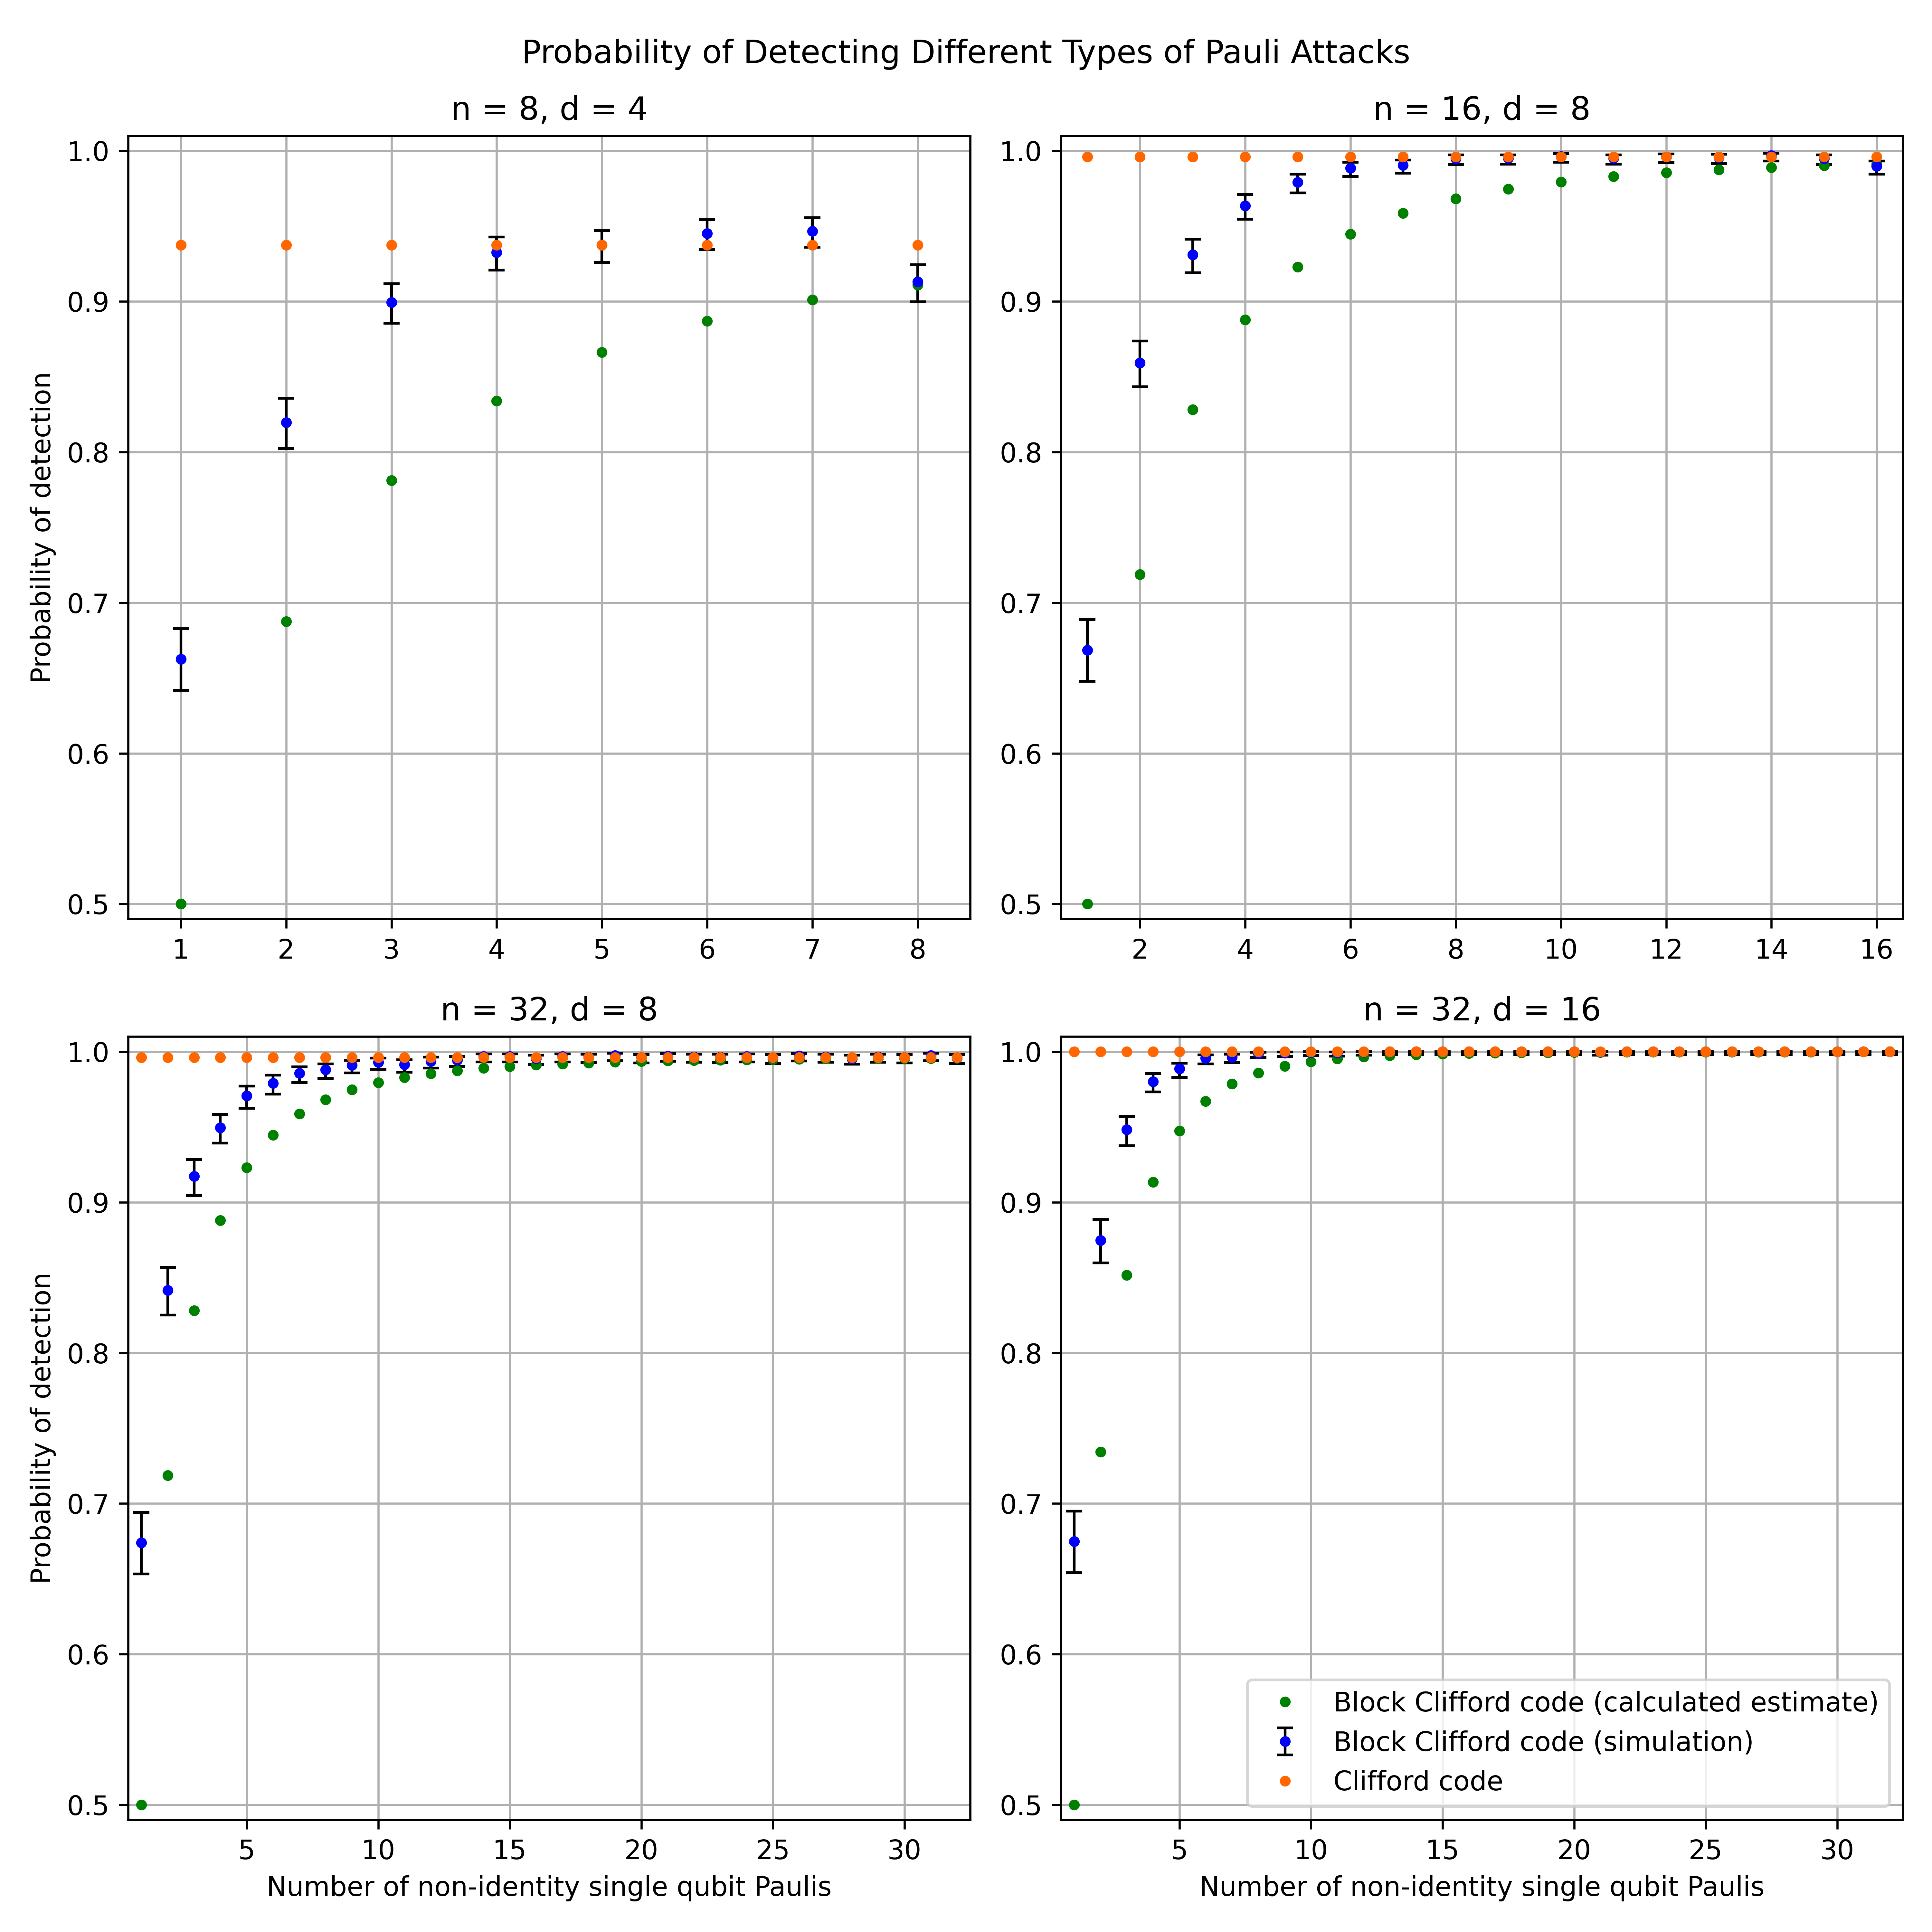
\includegraphics[scale=0.6]{Figures/multi_graph_pauli_attacks.png}
    \caption{Figures showing the probability of detection for the Clifford code and the block Clifford code. Each $x$ value on the $x$-axis denotes an adversary attacking only using random Paulis from $P(n)$ containing $x$ number of non-identity single-qubit Paulis.}
    \label{fig:multiGraphPaulAttacks}
\end{figure}

Figure~\ref{fig:multiGraphPaulAttacks} compares the probability of detection for the Clifford code and the block Clifford code. Each subgraph corresponds to an experiment. The title for each subgraph depicts the values of $n$ and $d$ for each experiment. The horizontal sequence of dots (orange) is the probability of detection for the Clifford code given by Equation~\eqref{eq:CliffordCodeProbabilityOfDetection}. The curved sequence of dots (blue) that has error bars on it depicts a confidence interval of $99.9 \%$ based on the Wilson score interval~\cite{wilsonScoreInterval}; it shows the results from a simulation of the block Clifford code with $5000$ trials for each $x$ value on the graph. The Wilson score interval is a confidence interval used for distributions arising from Bernoulli trials (trials with an outcome of $1$ indicating success and $0$ indicating failure). In this case, $1$ denotes the adversary was detected in a trial and $0$ denotes the adversary was not detected in a trial. The curved sequence of dots (green) in Figure~\ref{fig:multiGraphPaulAttacks} without error bars is the approximated probability of detection for the block Clifford code given by Equation~\eqref{eq:stirlingNumberFunctionCombinedWithOtherTheorems}. 

For all experiments, the block Clifford code quickly approaches a probability of detection comparable to the Clifford code as the number of non-identity single-qubit Paulis, $x$, in the attack increases. The experiment with $n = 32$ and $d = 16$ had the block Clifford code detect all $5000$ attacks for $19$ out of the $32$ values of $x$.

\chapter{Conclusion}
\label{sec:Conclusion}
\section{Discussion}
\label{sec:Discussion}
\begin{figure}
    \centering
    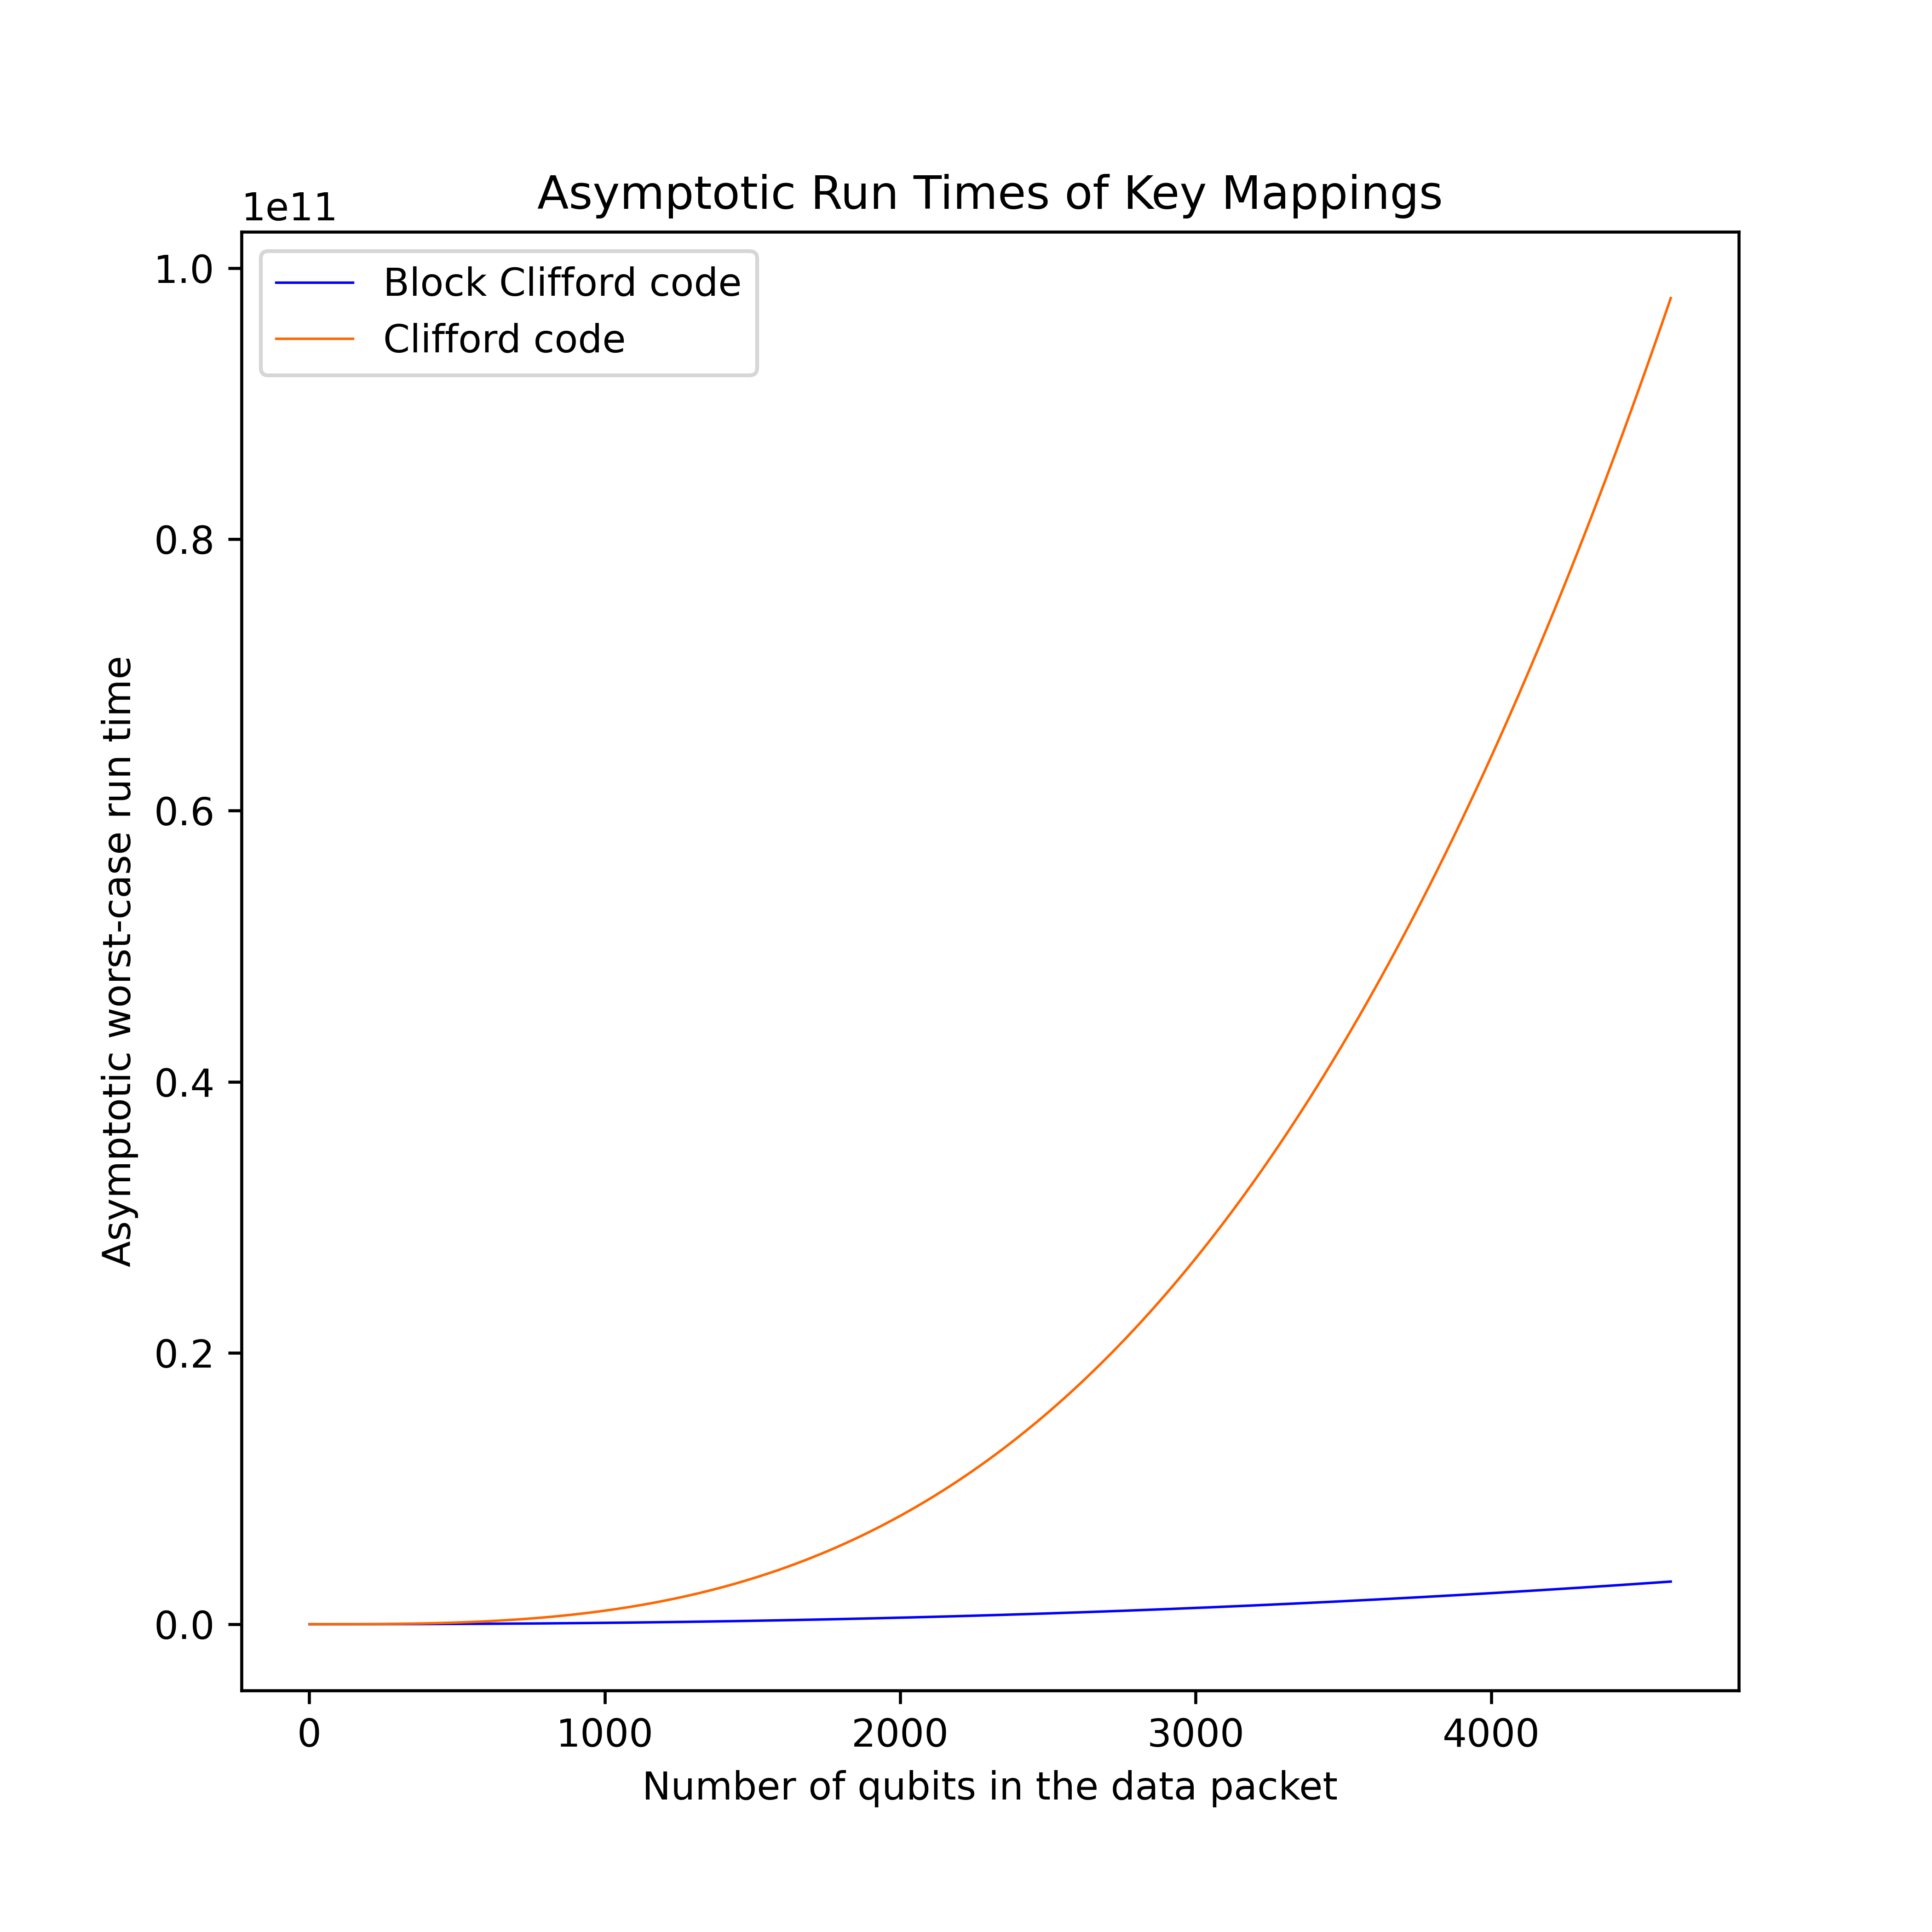
\includegraphics[scale=0.6]{Figures/keymapping_runtimes.png}
    \caption{A figure comparing $n^3$ (Clifford code) to $n^2 \log_2^2 (n)$ (block Clifford code).}
    \label{fig:keyMappingRunTimesComparison}
\end{figure}

The Clifford code's key mapping runs in $O\left(n^3\right)$ time, and the block Clifford code's key mapping runs in $O\left(n^2 \log_2^2 (n)\right)$ time. It is not yet known how large data packets in a quantum internet might be. However, in classical networks data packets can contain thousands of bits~\cite{rfc879}, which may indicate the size of packets in quantum networks of the future. Assuming quantum data packets will have thousands of qubits, one would want to invest in efficient key mappings. For example, if a data packet had $1000$ qubits, an $O\left(n^3\right)$ key mapping would result in a computation on the order of a billion operations. Although modern computers can perform these operations in a fraction of a second, it is still a relatively expensive operation for a computer to be performing frequently, especially in situations with stringent low latency requirements or limited computing power. Figure~\ref{fig:keyMappingRunTimesComparison} shows how much faster $n^3$ grows in comparison to $n^2 \log_2^2 (n)$.

\begin{myLemmarep}
$O\left(n^3\right)$ is asymptotically larger than $O\left(n^2 \log_2^2 (n)\right)$.
\end{myLemmarep}
\begin{proof}
First, some simplifications are made:
\begin{align}
n^2 \log_2^2 (n) &< n^3\\
\log_2^2 (n) &< n \\
\log_2 (n) &< \sqrt{n} \label{eq:simplifiedRunTimeComparison}
\end{align}
 The proof can be completed by using the racetrack principle. First, note that substituting $n = 16$ into Equation~\eqref{eq:simplifiedRunTimeComparison} shows that:
\begin{align}
\log_2 (16) = \sqrt{16}
\end{align}
Now, it must be shown that taking the derivatives of both sides of Equation~\eqref{eq:simplifiedRunTimeComparison} satisfies the inequality for all $n \geq 16$. Taking the derivatives of both sides gives:
\begin{align}
\frac{1}{n \ln (2)} &< \frac{1}{2\sqrt{n}}\\
\frac{2\sqrt{n}}{n \ln (2)} &< 1\\
\frac{4n}{n^2 (\ln^2 (2))} &< 1\\
\frac{4}{n (\ln^2 (2))} &< 1\\
\frac{4}{(\ln^2 (2))} \approx 8.33 &< n
\end{align}
Thus concluding the proof.
\end{proof}

In Section~\ref{subsec:noise} a type of noise called depolarizing noise was characterized. There is reason to believe that many applications in quantum computing will work well with noisy qubits~\cite{noisyQuantuamMachineLearning,sheldon2019quantum,rosch2022quantum,approximateQuantumComputing,noiseToTheirAdvantage}. Given this assumption, a protocol such as the block Clifford code which can accept data packets with one or two noisy qubits with non-negligible probability (remark Figure~\ref{fig:multiGraphPaulAttacks}) may be advantageous.

The block Clifford code also has a construction which uses $O\left(nd\right)$ gates from the Clifford generators. This construction may be optimal for certain values of $n$ and $d$; more investigation is needed. For a fixed $d$, this is certainly asymptotically less than the worst-case of $O\left(\frac{n^2}{\log_2^2 (n)}\right)$ for the Clifford code. Figure~\ref{fig:numberOfGatesComparison} shows how much faster $\frac{n^2}{\log_2 (n)}$ grows in comparison to $nd$ with $d= 64$.

\begin{figure}
    \centering
    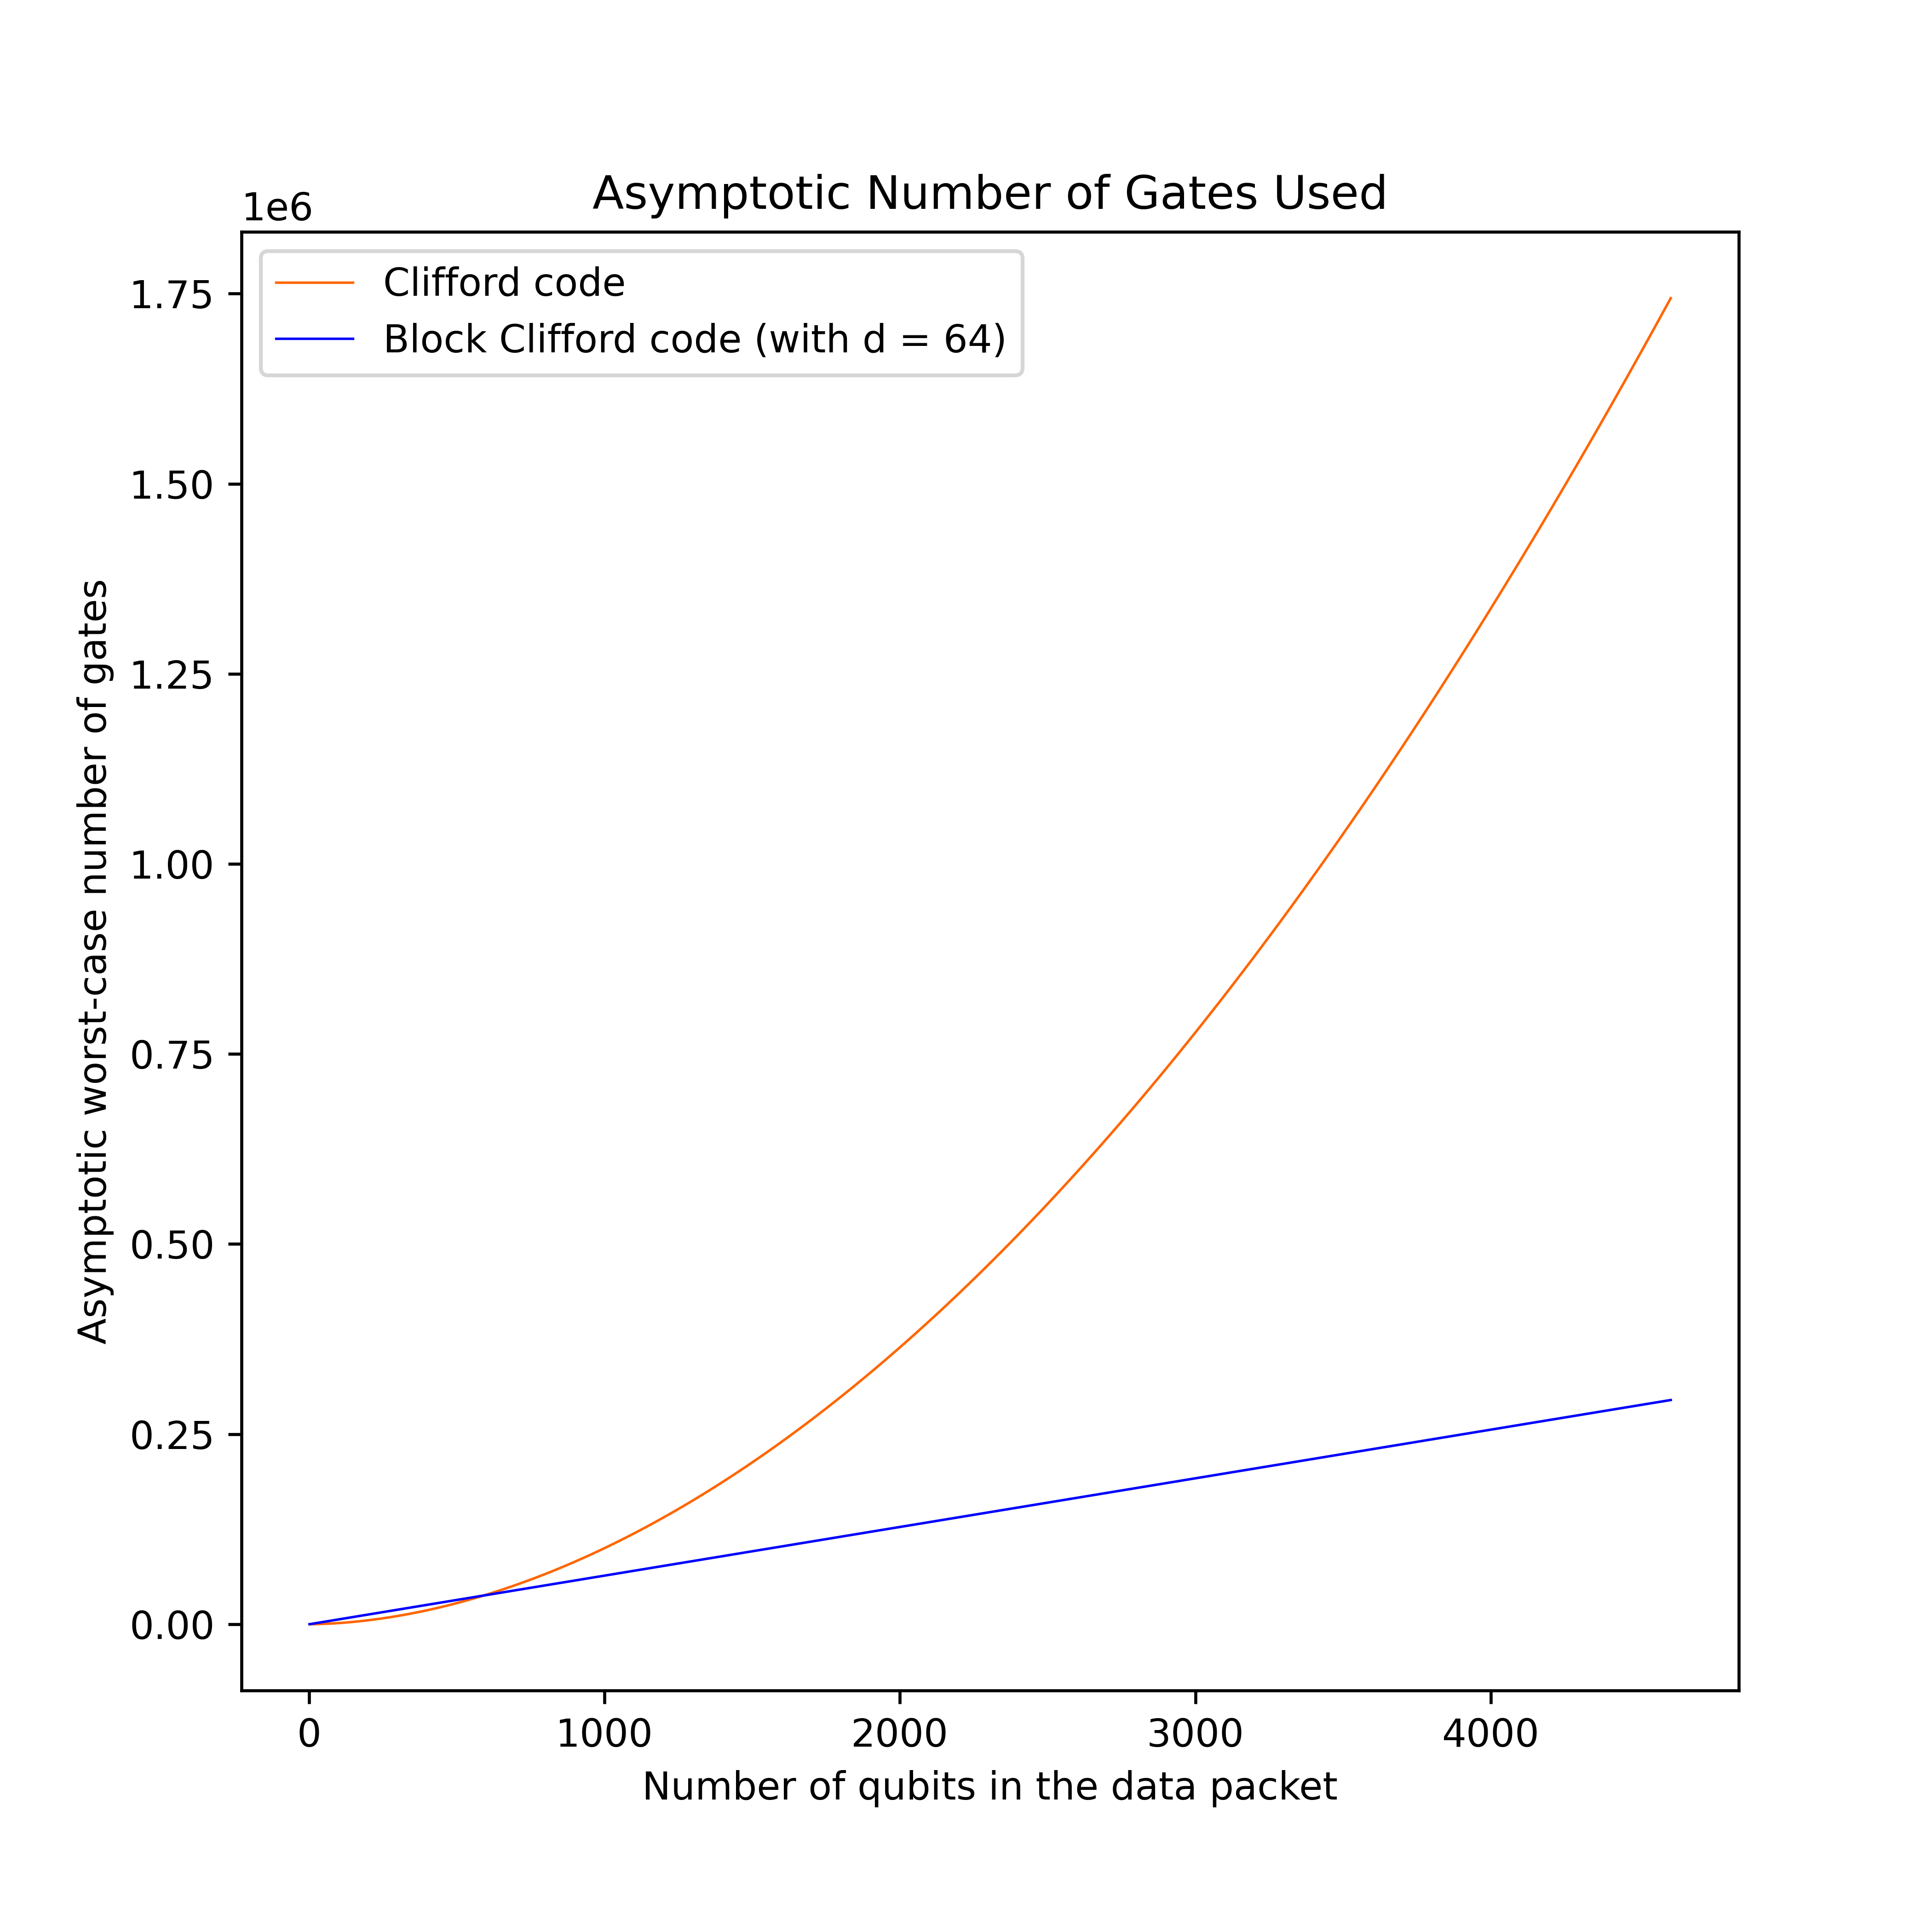
\includegraphics[scale=0.6]{Figures/number_of_gates.png}
    \caption{A figure comparing $\frac{n^2}{\log_2 (n)}$ (Clifford code) to $nd$ (block Clifford code).}
    \label{fig:numberOfGatesComparison}
\end{figure}

\section{Future Work}
More precisely characterizing how the block Clifford code handles noisy data may be the focus of future work. Finding an exact (as opposed to an approximate) characterization of the block Clifford code's security would be beneficial. 

The time complexity of the key mapping method for the block Clifford code could potentially be reduced. One way to tackle this problem would be to increase the memory it uses, in hopes that it will increase computational efficiency. The subkey $k_a$ mapping could be sped up by assigning groupings of two adjacent bits in the binary key to each single-qubit unitary. The mapping could read the groupings of two bits from the key sequentially, where $00$, $01$ and $10$ could correspond to each of $I$, $H$, and $S^{\dagger}H$. A grouping with $11$ could correspond to the single-qubit unitary determined by the previously read grouping of two bits. If $11$ were the first read grouping of bits, it could be assigned $I$. This would cause more key collisions, but could still determine an essentially uniform distribution of unitaries to apply to the packet. The subkey $k_b$ mapping could be sped up by computing all the ${m \choose j}$s ahead of time and storing them in memory so that they don't have to be calculated every time the subkey mapping is computed. 

The multiset permutation unranking algorithm may also be extended to describe a multiset permutation ranking algorithm. The unranking algorithm may be used to fully describe the key mapping for the trap code as well.




%\appendix
%\chapter{Appendix}
% Input Appendix chapters: \input{chapters/appendix}

% Bibliography
%trying to change the style
%\addbibresource{bibliography.bib}
%\printbibliography

\bibliographystyle{unsrt}
\bibliography{bibliography}

\end{document}